%!%!TEX TS-program = pdflatex
%!TEX encoding = utf8 
\documentclass[12pt, oneside, openany]{book}
\usepackage[T1]{fontenc}
\usepackage[utf8]{inputenc}
\usepackage[english, spanish, es-noshorthands]{babel}
%% FONTS: libertine+biolinum+stix
\usepackage[mono=false]{libertine}
\usepackage[notext]{stix}
\usepackage{pgfplots}
\pgfplotsset{compat=1.18}
% =====================
% = Datos importantes =
% =====================
% hay que rellenar estos datos y luego
% ir a \begin{document}

\title{Fundamentos Matem\'aticos de los Energy-Based Models y las Joint Embedding Architectures}
\newcommand{\mysubtitle}[1]{\newcommand{\guardasubtitle}{#1}}
\mysubtitle{Del Representation Collapse a los World Models}
\author{\large Pedro Rivas Vega}
\date{\today}
\newcommand{\tutores}[1]{\newcommand{\guardatutores}{#1}}
\tutores{Prof. Eduardo Sánchez Karhunen\\}
% Definición
\newcommand{\departamento}[2]{\newcommand{\guardadepartamento}{#2}}

% Uso (el primer argumento #1 parece ignorado en tu definición actual, 
% pero pasas el nombre del departamento como #2)
\departamento{CCIA}{Ciencias de la Computación e Inteligencia Artificial\\}

% ======================
% = Páginas de títulos =
% ======================
\makeatletter
\edef\maintitle{\@title}
\renewcommand\maketitle{%
  \begin{titlepage}
      \vspace*{1.5cm}
      \parskip=0pt
      \Huge\bfseries
      \begin{center}
          \leavevmode
\includegraphics[totalheight=6cm]{sello.pdf}\\[2cm]
          \@title\\[0.5cm]
          {\Large\normalfont\guardasubtitle}
      \end{center}
      \vspace{1cm}
      \begin{center}
          \@author
      \end{center}
  \end{titlepage}
  
  \begin{titlepage}
  \parindent=0pt
  \begin{flushleft}
  \vspace*{1.5mm}
  \setlength\baselineskip{0pt}
  \setlength\parskip{0mm}
  \begin{center}
      \leavevmode
\includegraphics[totalheight=4.5cm]{sello.pdf}
  \end{center}
  \end{flushleft}
  \vspace{1cm}
  \bgroup
  \Large \bfseries
  \begin{center}
  \@title\\[0.4cm]
  {\large\normalfont\guardasubtitle}
  \end{center}
  \egroup
  \vspace*{.5cm}
  \begin{center}
  \@author
  \end{center}
  \vspace*{1.8cm}
  \begin{flushright}
  \begin{minipage}{8.45cm}
      Memoria presentada como parte de los requisitos para la obtención del título de
      Grado en Matemáticas por la Universidad de Sevilla.

      \vspace*{7.5mm}

      Tutorizada por
      % \vspace*{5mm}
  \end{minipage}\par
  \begin{tabularx}{8.45cm}[b]{@{}l}
      \guardatutores
      \guardadepartamento
  \end{tabularx}
  \end{flushright}
      \vspace*{\fill}
   \end{titlepage}
   

   %%% Esto es necesario...
   \pagestyle{tfg}
   \renewcommand{\chaptermark}[1]{\markright{\thechapter.\space ##1}}
   \renewcommand{\sectionmark}[1]{}
   \renewcommand{\subsectionmark}[1]{}
  }
\makeatother

% ======================================
% = Color de la Universidad de Sevilla =
% ======================================
\usepackage{tikz}
\usepackage{pgfplots}
\pgfplotsset{compat=1.18}
\usetikzlibrary{arrows.meta, shadows, positioning, calc, matrix, shapes.geometric, backgrounds, fit}
\definecolor{USred}{cmyk}{0,1.00,0.65,0.34}

% =========
% = Otros =
% =========
\usepackage[]{tabularx}
\usepackage[]{enumitem}
\setlist{noitemsep}
\usepackage{url}           % para \url{} en entradas BibTeX
\usepackage[font=footnotesize]{caption} % Tamaño pequeño para los pies de figura
\usepackage[bottom]{footmisc} % Obliga a que las notas al pie estén siempre pegadas al margen inferior
\usepackage{float} % Permite usar [H] para forzar la posición de las figuras

% ==========================
% = Matemáticas y teoremas =
% ==========================
\usepackage[]{amsmath}
\usepackage[]{amsthm}
\usepackage[]{mathtools}
\usepackage[]{bm}
\usepackage[]{thmtools}

% ── Cajas destacadas (notas del paper) ──────────────────────
\usepackage[most]{tcolorbox}
\definecolor{miBorde}{HTML}{941120}
\newtcolorbox{mybox}{
    colback=miBorde!5!white,
    colframe=miBorde,
    arc=3pt,
    boxrule=1.2pt,
    fontupper=\small\sffamily,
    left=8pt, right=8pt, top=6pt, bottom=6pt
}
\newcommand{\marcador}{\vrule height 10pt depth 2pt width 2pt \hskip .5em\relax}
\newcommand{\cabeceraespecial}{%
    \color{USred}%
    \normalfont\bfseries}
\declaretheoremstyle[
    spaceabove=\medskipamount,
    spacebelow=\bigskipamount,
    headfont=\cabeceraespecial\marcador,
    notefont=\cabeceraespecial,
    notebraces={(}{)},
    bodyfont=\normalfont\itshape,
    postheadspace=1em,
    numberwithin=chapter,
    headindent=0pt,
    headpunct={.}
    ]{importante}
\declaretheoremstyle[
    spaceabove=\medskipamount,
    spacebelow=\bigskipamount,
    headfont=\normalfont\itshape\color{USred},
    notefont=\normalfont,
    notebraces={(}{)},
    bodyfont=\normalfont,
    postheadspace=1em,
    numberwithin=chapter,
    headindent=0pt,
    headpunct={.}
    ]{normal}
\declaretheoremstyle[
    spaceabove=\medskipamount,
    spacebelow=\bigskipamount,
    headfont=\normalfont\itshape\color{USred},
    notefont=\normalfont,
    notebraces={(}{)},
    bodyfont=\normalfont,
    postheadspace=1em,
    headindent=0pt,
    headpunct={.},
    numbered=no,
    qed=\color{USred}\marcador
    ]{demostracion}

% Los nombres de los enunciados. Añade los que necesites.
\declaretheorem[name=Observaci\'on, style=normal]{remark}
\declaretheorem[name=Corolario, style=normal]{corollary}
\declaretheorem[name=Proposici\'on, style=normal]{proposition}
\declaretheorem[name=Lema, style=normal]{lemma}
\declaretheorem[name=Ejemplo, style=normal]{example}

\declaretheorem[name=Teorema, style=importante]{theorem}
\declaretheorem[name=Definici\'on, style=importante]{definition}

\let\proof=\undefined
\declaretheorem[name=Demostraci\'on, style=demostracion]{proof}

% ============================
% = Hipervínculos (hyperref) =
% ============================
\usepackage[
    colorlinks=true,
    linkcolor=USred,
    citecolor=USred,
    urlcolor=USred,
    bookmarksnumbered=true,
    pdfencoding=auto,
    unicode=true
]{hyperref}


% ============================
% = Composición de la página =
% ============================
\usepackage[
	a4paper,
    textwidth=80ex,
]{geometry}

\linespread{1.069}
\parskip=10pt plus 1pt minus .5pt
\frenchspacing
% \raggedright

% Margen vertical adicional para figuras
\setlength{\intextsep}{\bigskipamount}
\setlength{\textfloatsep}{\bigskipamount}


% ==============================
% = Composición de los títulos =
% ==============================

\usepackage[explicit]{titlesec}

\newcommand{\hsp}{\hspace{20pt}}
\titleformat{\chapter}[hang]
    {\Huge\sffamily\bfseries}
    {\thechapter\hsp\textcolor{USred}{\vrule width 2pt}\hsp}{0pt}
    {#1}
\titleformat{\section}
  {\normalfont\Large\sffamily\bfseries}{\thesection\space\space}
  {1ex}
  {#1}
\titleformat{\subsection}
  {\normalfont\large\sffamily\bfseries}{\thesubsection\space\space}
  {1ex}
  {#1}

% =======================
% = Cabeceras de página =
% =======================
\usepackage[]{fancyhdr}
\usepackage[]{emptypage}
\fancypagestyle{plain}{%
    \fancyhf{}%
    \renewcommand{\headrulewidth}{0pt}
    \renewcommand{\footrulewidth}{0pt}
}
\fancypagestyle{tfg}{%
    \fancyhf{}%
    \renewcommand{\headrulewidth}{0pt}
    \renewcommand{\footrulewidth}{0pt}
    \fancyhead[LE]{{\normalsize\color{USred}\bfseries\thepage}\quad
                    \small\textsc{\MakeLowercase{\maintitle}}}
    \fancyhead[RO]{\small\textsc{\MakeLowercase{\rightmark}}%
                    \quad{\normalsize\bfseries\color{USred}\thepage}}%
                    }

% =============================
% = El documento empieza aquí =
% =============================
\begin{document}



\maketitle

\frontmatter

\tableofcontents

\mainmatter

\chapter*{Resumen}
\addcontentsline{toc}{chapter}{Resumen}
\markright{Resumen}
Si se observa el aprendizaje en la naturaleza, en el desarrollo cognitivo de un niño, en la adquisición del lenguaje, en la formación gradual del sentido común resulta razonable conjeturar que la mayor parte del conocimiento se adquiere por la mera observación del mundo, sin etiquetas ni recompensas externas. Solo una fracción pequeña proviene de la interacción supervisada con un instructor, y una parte aún más reducida del ensayo y error deliberado. Esta jerarquía de observación, supervisión, exploración coincide con la ``Analogía del Pastel'' de Yann LeCun, que situó el \textbf{aprendizaje auto-supervisado} (SSL) como el cuerpo esencial de todo sistema cognitivo eficiente. La hipótesis de fondo es que de este proceso de observación pura emergen los conceptos abstractos que estructuran el entendimiento del mundo: no como réplicas del estímulo sensorial, sino como abstracciones de sus relaciones invariantes.

Esta hipótesis ha sido verificada con éxito sobre el lenguaje natural. El lenguaje constituye un proxy simbólico del mundo real: dominio es discreto, dimensionalidad manejable, y la tarea de predecir el siguiente token codifica implícitamente la estructura semántica y lógica de la realidad. Sobre esta base, los \textit{Large Language Models} (LLM) han demostrado que el SSL a escala produce capacidades de razonamiento emergentes de una potencia sin precedentes. La pregunta que abre este trabajo es, por tanto, inevitable: \textit{¿cómo trasladar este mismo razonamiento a datos mucho más cercanos al mundo físico, como visión, vídeo, datos espaciales o datos de interacción, que son continuos, de alta dimensionalidad y carecen de un token natural?}

Para responderla, este trabajo explora un paradigma que lleva rondando desde los años noventa, silencioso y paralelo a los enfoques discriminativos y generativos que han dominado la historia del aprendizaje automático: las \textbf{Joint Embedding Architectures} (JEA). Lejos de reconstruir el mundo o de clasificarlo, las JEA aprenden a proyectar observaciones correlacionadas a un espacio latente compartido donde la compatibilidad semántica reemplaza a la similitud superficial. Este principio, enunciado por primera vez en el contexto de las redes siamesas de Bromley y LeCun en 1993, permaneció durante décadas en los márgenes de la investigación. Hoy, con el impulso de la escala computacional y la madurez teórica, se erige como una de las piezas más prometedoras para construir sistemas capaces de razonar, predecir las consecuencias de sus acciones y actuar de forma autónoma en el mundo físico. El marco teórico que las unifica es el de los \textbf{Modelos Basados en Energía} (EBM): funciones de compatibilidad no normalizadas cuya función de partición resulta analíticamente intratable en el dominio continuo de la visión, en contraste con el escenario discreto y tratable del softmax en los LLM, y cuya forma óptima queda fundamentada, como se demuestra en este trabajo, en el Principio de Máxima Entropía de Jaynes.

El recorrido que propone esta memoria es un \textit{viaje evolutivo}: desde las primeras redes siamesas y el problema del colapso trivial de la representación, problema central que articula toda la obra, hasta las soluciones contrastivas, las regularizaciones matriciales no contrastivas de Barlow Twins y VICReg, los mecanismos ad-hoc de V-JEPA, y finalmente \textbf{LeWorldModel}: una síntesis que reduce toda la regularización a un único funcional escalar fundado en el Teorema de Cramér-Wold, y que habilita la planificación autónoma por control óptimo en entornos visuales complejos. El trabajo concluye mirando al futuro con una pregunta que el propio paradigma plantea, y quizás con algo de vértigo histórico. Las redes convolucionales de LeCun, formuladas en los años ochenta, esperaron casi cuatro décadas hasta que la escala computacional les dio la razón. ¿Será el destino de las JEA, nacidas en esa misma época, repetir esa trayectoria? ¿Estaremos asistiendo, de nuevo, al comienzo silencioso de la próxima revolución?

\chapter*{Abstract}
\addcontentsline{toc}{chapter}{Abstract}
\markright{English Abstract}
\begin{otherlanguage}{english}
If one observes learning as it occurs in nature, in the cognitive development of a child, in the acquisition of language, in the gradual formation of common sense, it becomes reasonable to conjecture that the majority of knowledge is acquired through pure observation of the world, without external labels or rewards. Only a small fraction arises from supervised interaction with a teacher, and an even smaller portion from deliberate trial and error. This hierarchy: observation, supervision, exploration, mirrors Yann LeCun's ``Cake Analogy,'' which placed \textbf{Self-Supervised Learning} (SSL) as the essential substance of any efficient cognitive system. The underlying hypothesis is that, from this process of unsupervised observation, abstract concepts emerge within the network's internal representation space, not as replicas of sensory stimuli, but as abstractions of their invariant relational structure.

This hypothesis has been verified with extraordinary success on natural language. Language constitutes a symbolic proxy for the real world: its domain is discrete, its dimensionality manageable, and the task of predicting the next token implicitly encodes the semantic and logical structure of reality. On this foundation, Large Language Models (LLMs) have demonstrated that SSL at scale produces emergent reasoning capabilities of unprecedented power. The question that opens this thesis is therefore unavoidable: \textit{how can this same reasoning be extended to data far closer to the physical world (vision, video, spatial data, interaction data) which are continuous, high-dimensional, and lack a natural token structure?}

To address it, this thesis explores a paradigm that has lingered since the nineteen-nineties, quiet and parallel to the discriminative and generative approaches that have dominated the history of machine learning: \textbf{Joint Embedding Architectures} (JEAs). Rather than reconstructing the world or classifying it, JEAs learn to project correlated observations into a shared latent space where semantic compatibility replaces superficial similarity. This principle, first articulated in the context of Bromley and LeCun's Siamese networks in 1993, remained at the margins of research for decades. Today, driven by computational scale and theoretical maturity, it stands as one of the most promising building blocks for systems capable of reasoning, predicting the consequences of their actions, and acting autonomously in the physical world. The theoretical framework that unifies them is that of \textbf{Energy-Based Models} (EBMs): unnormalized compatibility functions whose partition function is analytically intractable in the continuous visual domain---in sharp contrast to the discrete, tractable softmax of LLMs---and whose optimal form is grounded, as this thesis demonstrates, in Jaynes' Principle of Maximum Entropy.

The journey this thesis proposes is an \textit{evolutionary one}: from the first Siamese networks and the problem of trivial representation collapse---the central problem articulating the entire work---through contrastive solutions, the non-contrastive matrix regularizations of Barlow Twins and VICReg, the ad-hoc mechanisms of V-JEPA, and finally \textbf{LeWorldModel}: a synthesis that reduces all regularization to a single scalar functional grounded in the Cram\'er-Wold Theorem, and that enables autonomous planning through optimal control in complex visual environments. The thesis concludes by looking toward the future with a question the paradigm itself raises---and perhaps with a certain historical vertigo. LeCun's convolutional networks, formulated in the nineteen-eighties, waited nearly four decades for computational scale to vindicate them. Will the JEAs, born in that same era, follow the same trajectory? Are we witnessing, once again, the quiet beginning of the next revolution?
\end{otherlanguage}


\chapter{Introducción y Fundamentos de Representation Learning}
\label{cap:intro}

El aprendizaje automático ha experimentado una transición en su objeto de estudio, pasando de optimizar fronteras de decisión supervisadas, a construir representaciones abstractas de los datos. En este capítulo introducimos los fundamentos del \textit{Representation Learning}, y presentamos los motivos por los que el paradigma JEA elude las limitaciones formales de los enfoques generativos y discriminativos tradicionales.

\section{Espacio Latente y Reducción de la Dimensionalidad}
\label{sec:espacio_latente}

El objetivo central del \textit{Representation Learning} es construir un modelo paramétrico $f_\theta: \mathcal{X} \to \mathcal{Z}$ que proyecte datos desde un espacio de observación de alta dimensionalidad $\mathcal{X} \subseteq \mathbb{R}^D$ (siendo $D$ el número de píxeles, frecuencias o características "crudas") hacia un espacio $\mathcal{Z} \subseteq \mathbb{R}^d$, con $d \ll D$, que llamaremos espacio latente, espacio de embeddings o espacio de representaciones. El elemento clave es que este modelo no es diseñado manualmente, sino que sus parámetros $\theta$ se optimizan de forma iterativa, generando representaciones en $\mathcal{Z}$ que codifican conceptos abstractos (p.e. identidad, categoría o relación causal), representaciones no explícitamente presentes en los datos de entrada.

\begin{definition}[Espacio Latente, Encoder y Mapeo de Embedding]
Sea $\mathcal{X}$ el espacio de entrada y $(\mathcal{Z}, d_{\mathcal{Z}})$ el espacio latente, tomado como el espacio euclídeo $\mathbb{R}^d$ dotado de la distancia euclídea estándar $d_{\mathcal{Z}}(a,b) = \|a - b\|_2$. Definimos el encoder como una aplicación parametrizada $f_{\theta}: \mathcal{X} \to \mathcal{Z}$, donde $\theta \in \Theta$ representa el conjunto de parámetros (p.e. pesos de una red neuronal). Para cada elemento $x \in \mathcal{X}$, su imagen $z = f_{\theta}(x) \in \mathcal{Z}$ recibe el nombre de embedding de $x$.
\end{definition}

Geométricamente, denotamos como $\mathcal{Z} = f_{\theta}(\mathcal{X})$ al conjunto de todas las representaciones generadas por la red. Este conjunto $\mathcal{Z} \subseteq \mathbb{R}^d$ habita dentro de un espacio vectorial euclídeo de dimensión $d$, siendo $d$, el número de neuronas de la capa de salida del encoder (Apéndice~\ref{ap:fundamentos_dl}).

\section{Tres Paradigmas: Discriminativo, Generativo y Joint Embedding}
\label{sec:tres_paradigmas}

Antes de estudiar por qué las \textit{Joint Embedding Architectures} constituyen una base adecuada para el \textit{representation learning}, y por tanto, para la construcción del espacio $\mathcal{Z}$, conviene analizar el contexto en el que se enmarcan en relación con los enfoques más tradicionales.


\subsection{El Enfoque Discriminativo}
Los modelos discriminativos tienen como objetivo estimar la distribución de probabilidad condicional de una variable objetivo o etiqueta $y \in \mathcal{Y}$ condicionada a un dato de entrada $x \in \mathcal{X}$:
\begin{equation}
p(y \mid x) = \frac{p(x, y)}{p(x)}
\end{equation}
donde $p(x,y)$ denota la densidad conjunta de etiquetas y datos, y donde $p(x)$ es la densidad marginal de las observaciones. Para ilustrar este paradigma, consideremos dos escenarios típicos de aplicación:
\begin{itemize}
    \item \textbf{Clasificación de imágenes:} El espacio de entrada $\mathcal{X} = [0, 1]^{H \times W \times C}$ representa imágenes de dimensión $H \times W$ con $C$ canales de color, mientras que el espacio de etiquetas es discreto y finito, $\mathcal{Y} = \{1, 2, \dots, K\}$, donde $K$ representa categorías mutuamente excluyentes. El objetivo consiste en estimar la probabilidad $p(y = k \mid x)$ para cada clase $k \in K$.
    \item \textbf{Regresión (p.e. la típica valoración inmobiliaria):} El espacio de entrada $\mathcal{X} \subset \mathbb{R}^D$ codifica $D$ características físicas y/o históricas de un inmueble (superficie, antigüedad, ubicación geográfica, número de estancias), mientras que el espacio de salida es continuo, $\mathcal{Y} = \mathbb{R}^+$, correspondiente a su precio de mercado. En este caso, el modelo estima el valor esperado del inmueble condicionado a sus características, es decir, la esperanza condicional $\mathbb{E}[y \mid x]$.
\end{itemize}
Aunque el modelado discriminativo constituye el pilar del aprendizaje supervisado tradicional \cite{goodfellow2016deep} y es altamente efectivo para resolver tareas de predicción específicas, presenta limitaciones para el aprendizaje de representaciones generales de los datos \cite{bengio2013representation}. En primer lugar, su formulación supervisada habitual, depende de un supervisor humano que suministre las etiquetas en $\mathcal{Y}$, un factor limitante en términos de escalabilidad y coste (computacional y humano) \cite{lecun2022path}. En segundo lugar, y desde una perspectiva de teoría de la información, en concordancia con el principio del cuello de botella de la información \cite{tishby2000information}, al optimizar el modelo exclusivamente para predecir la variable objetivo, los gradientes fuerzan a la red a descartar toda variabilidad y estructura geométrica de $\mathcal{X}$ que no sea estrictamente útil para resolver la tarea en cuestión. El descarte de características que pueden ser valiosas para tareas secundarias o futuras, motivó la búsqueda de paradigmas auto-supervisados, que fueran capaces de extraer regularidades directamente de la propia estructura de los datos \cite{bengio2013representation}, dando paso inicialmente al modelado generativo.


\subsection{El Enfoque Generativo}
\label{subsec:generativo}
El enfoque generativo tiene como objetivo modelar la distribución de probabilidad de los datos de manera que le permita generar o reconstruir muestras en el espacio original $\mathcal{X}$. Este paradigma es la base del éxito de los modelos fundacionales modernos, ya sean arquitecturas autorregresivas (tipo GPT) utilizadas en el procesamiento del lenguaje o modelos de difusión utilizados para la generación de imágenes. Sin embargo, forzar al sistema a generar o reconstruir el entorno puede resultar ineficiente. 

Para razonar y ``pensar'' sobre el mundo no parece imprescindible recrearlo a nivel de píxeles o detalles físicos, bastaría con operar sobre representaciones abstractas de sus conceptos. De hecho, los modelos generativos desarrollan y utilizan estas representaciones abstractas en sus capas intermedias para guiar el proceso. Pero el paradigma obliga a materializarlas y concretarlas en reconstrucciones explícitas en el espacio original $\mathcal{X}$, introduciendo ineficiencias. Por ejemplo, para decidir si es seguro cruzar una calle, es necesario predecir la trayectoria futura y el comportamiento del vehículo que se aproxima; resulta ineficiente que el modelo se vea forzado a concretar esa predicción determinando p.e. el movimiento del paisaje de fondo. El modelado generativo obliga a consumir importantes recursos computacionales en representar estos detalles estocásticos, en lugar de concentrarse únicamente en la dinámica semántica y estructural de la escena en el espacio latente. Esta ineficiencia motivó la búsqueda de alternativas que eviten por completo esta fase de reconstrucción física.

\subsection{El Paradigma Joint Embedding Architectures (JEA)}
El paradigma de \textit{Joint Embedding Architectures} elude por completo la fase de reconstrucción. En su lugar, el sistema toma dos entradas correlacionadas $x, y \in \mathcal{X}$ (p.e. dos transformaciones de una misma imagen, o dos fotogramas consecutivos de un vídeo), las proyecta a través de dos encoders $f_{\theta}: \mathcal{X} \to \mathcal{Z}$ y $g_{\phi}: \mathcal{X} \to \mathcal{Z}$, y minimiza la distancia entre sus representaciones en $\mathcal{Z}$:
\begin{equation}
\mathcal{L}_{\text{JEA}}(x, y) = \left\| f_{\theta}(x) - g_{\phi}(y) \right\|_2^2
\end{equation}
donde $\theta, \phi \in \Theta$ son los parámetros de cada encoder, que pueden ser compartidos ($\theta = \phi$) o independientes según la arquitectura concreta.

\begin{figure}[H]
\centering
\begin{tikzpicture}[node distance=1.5cm, auto, >=Stealth]
    \node (x) [draw, rectangle, minimum width=2.5cm, minimum height=1cm] {Entrada $x$};
    \node (y) [draw, rectangle, minimum width=2.5cm, minimum height=1cm, below=of x] {Entrada $y$};
    \node (fx) [draw, rectangle, minimum width=2cm, minimum height=1cm, right=of x, xshift=1cm] {Encoder $f_{\theta}$};
    \node (gy) [draw, rectangle, minimum width=2cm, minimum height=1cm, right=of y, xshift=1cm] {Encoder $g_{\phi}$};
    \node (zx) [circle, draw, right=of fx, xshift=1cm] {$z_x$};
    \node (zy) [circle, draw, right=of gy, xshift=1cm] {$z_y$};
    \node (loss) [draw, diamond, minimum width=1.5cm, minimum height=1.5cm, right=of zx, yshift=-1.1cm, xshift=1cm] {Loss}; 

    \draw[->] (x) -- (fx);
    \draw[->] (y) -- (gy);
    \draw[->] (fx) -- (zx);
    \draw[->] (gy) -- (zy);
    \draw[->] (zx) -| (loss);
    \draw[->] (zy) -| (loss);
    \draw[dashed, <->] (fx) -- node[left] {Shared $\theta$ (opcional)} (gy);
\end{tikzpicture}
\caption{Diagrama conceptual de una Joint Embedding Architecture (JEA). Los encoders $f_\theta$ y $g_\phi$ proyectan las entradas correlacionadas al espacio latente $\mathcal{Z}$; la pérdida penaliza la distancia entre sus representaciones. El intercambio de parámetros (indicado con línea discontinua) es opcional y depende de la arquitectura concreta.}
\label{fig:jea_diagram}
\end{figure}

En general, los encoders $f_{\theta}$ y $g_{\phi}$ pueden tener diferentes parámetros. Sin embargo, en la mayoría de implementaciones prácticas, ambos encoders comparten los mismos pesos ($\theta = \phi$). Esto garantiza que la función de proyección sea idéntica para ambas ramas, de modo que entradas iguales producen necesariamente el mismo embedding.

Al no requerir un decoder que opere en $\mathbb{R}^D$, las JEA no invierten capacidad del modelo en detalles irrelevantes para la tarea, como los que hemos comentado anteriormente. Este encoder actúa a modo de filtro que retiene únicamente la información semánticamente relevante, estructurando el espacio $\mathcal{Z}$ de manera tal que la similaridad geométrica refleje similaridad semántica.

Sin embargo, este paradigma plantea importantes interrogantes. En primer lugar, ¿Garantiza el proceso de optimización que la representación obtenida recupere fielmente los verdaderos grados de libertad del mundo físico (las variables latentes generadoras), o corre el riesgo de distorsionarlas de forma que pierdan su estructura? Este es el problema del \emph{colapso de las representaciones} \cite{jing2022understanding}. En segundo lugar; ¿es posible planificar y controlar un agente de forma óptima en este espacio sin degradar su rendimiento real? En el Capítulo~\ref{cap:modelos_mundo} se introduce la dimensión temporal incorporando una ventana de planificación dentro de estos espacios latentes y se analizan las soluciones de tipo JEPA desarrolladas para evitar el colapso. Por su parte, en el Capítulo~\ref{cap:leworldmodel} explora la solución de regularización isótropa (SIGReg) propuesta en 2025 \cite{balestriero2025lejepa} como evolución para superar los métodos matriciales de tipo VICReg marcando el camino hacia la planificación en el espacio $\mathcal{Z}$.

En este trabajo abordamos la trayectoria histórica y conceptual que ha permitido consolidar el paradigma de las Joint Embedding Architectures. El hilo conductor es la resolución del problema más persistente de este paradigma: el \textbf{representation collapse}, donde la red minimiza la energía a cero mapeando todas las entradas a una constante trivial $f_{\theta}(x) = c$. La noción central es la de \emph{compatibilidad}: una medida no normalizada que cuantifica el grado de correspondencia semántica entre dos variables de entrada, y cuya formalización mediante funciones de energía se desarrolla en el capítulo siguiente donde se introduce formalmente los Modelos Basados en Energía (EBM) como marco unificador para el aprendizaje de compatibilidades, comparando los escenarios discretos y continuos, y sentando las bases físicas del Principio de Máxima Entropía de Jaynes.
\chapter{Modelos Basados en Energía y Aprendizaje de Compatibilidades}
\label{cap:ebm_compatibilidades}

\input{cap2_introEBM}
\section{Introducción a los Energy-Based Models y el Paisaje de Energía}
\label{sec:intro_ebm}

Los Modelos Basados en Energía (EBM) ofrecen un marco matemático flexible para el diseño de sistemas de inteligencia artificial \cite{lecun2006tutorial}. En el contexto de este trabajo, constituyen la base formal de las \textbf{Joint Embedding Architectures (JEA)}. A diferencia de los modelos probabilísticos, que requieren una  normalización estricta, los EBM evalúa la compatibilidad entre variables asignándoles un escalar no normalizado denominado "energía". Intuitivamente, una energía baja indica que la combinación de variables es altamente plausible o compatible, mientras que una energía alta denota incompatibilidad. Esta métrica se puede visualizar como un "paisaje de energía" donde los valles (mínimos locales) representan las configuraciones de interés, y las cimas (picos de energía) representan configuraciones "implausibles" o ruido. Si el modelo fracasa y mapea cualquier combinación a la misma energía (por ejemplo, a cero), el paisaje de energía se aplana completamente. Este  fenómeno destructivo se le conoce como \textbf{colapso de representación}.

\subsection{La Función de Energía y su Independencia Probabilística}
\label{sec:energy_function}

En tareas de predicción y aprendizaje de representaciones (como las JEA), el modelo opera sobre el espacio conjunto de configuraciones, definido como el espacio producto $\mathcal{C} = \mathcal{X} \times \mathcal{Y}$, donde $x \in \mathcal{X}$ representa la variable observada o entrada del sistema (por ejemplo, el contexto de una imagen o fotograma) e $y \in \mathcal{Y}$ es la predicción o variable de destino a evaluar, La pieza central del modelo es la función de energía condicional:
\begin{equation}
E_\theta(x, y) \in \mathbb{R}
\end{equation}
siendo $\theta$ los parámetros entrenables del modelo (pesos de la red neuronal). El escalar $E_\theta(x, y)$ mide directamente la \textbf{discrepancia} entre $x$ e $y$. Esta energía se caracteriza por su total independencia de los axiomas de Kolmogorov:
\begin{itemize}
    \item \textbf{No negatividad:} A diferencia de las densidades de probabilidad, $E_\theta(x, y)$ puede tomar valores reales negativos.
    \item \textbf{Normalización:} No requiere que la integral sobre el espacio de predicción sume la unidad: $\int_{\mathcal{Y}} E_\theta(x, y') \, dy' \neq 1$.
\end{itemize}

Esta flexibilidad permite a las JEA centrarse exclusivamente en la superficie de energía, evitando calcular constantes de normalización complejas y canalizando la capacidad del modelo a la dinámica semántica de los datos en sus representaciones.

\subsection{Inferencia en Modelos Basados en Energía}
Realizar inferencia en un EBM consiste en buscar el estado \textbf{y} que minimiza la energía para una entrada observada $x$ dada. A diferencia del enfoque probabilístico que calcula expectativas o integrales sobre todo el espacio de salida, la inferencia no normalizada se reduce a un problema de optimización o búsqueda del mínimo global:
\begin{equation}
\label{eq:ebm_inferencia}
y^* = \arg\min_{y \in \mathcal{Y}} E_\theta(x, y)
\end{equation}

En la Figura~\ref{fig:ebm_inferencia_retriever}, se ilustra esta idea para el caso de clasificación de imágenes. Dada una entrada observada $x$ (la imagen de un perro), el modelo evalúa la energía $E_\theta(x, y)$ para cada una de las clases candidatas $y$. La respuesta inferida es la clase que produce el valor de energía mínimo (representado por la barra más corta).

\begin{figure}[H]
    \centering
    \begin{tikzpicture}[
        >=stealth,
        textfont/.style={font=\small\sffamily, align=center},
        labelsbox/.style={draw, align=left, inner sep=1.5ex, font=\small\sffamily, text depth=0pt}
    ]
        \node (img) {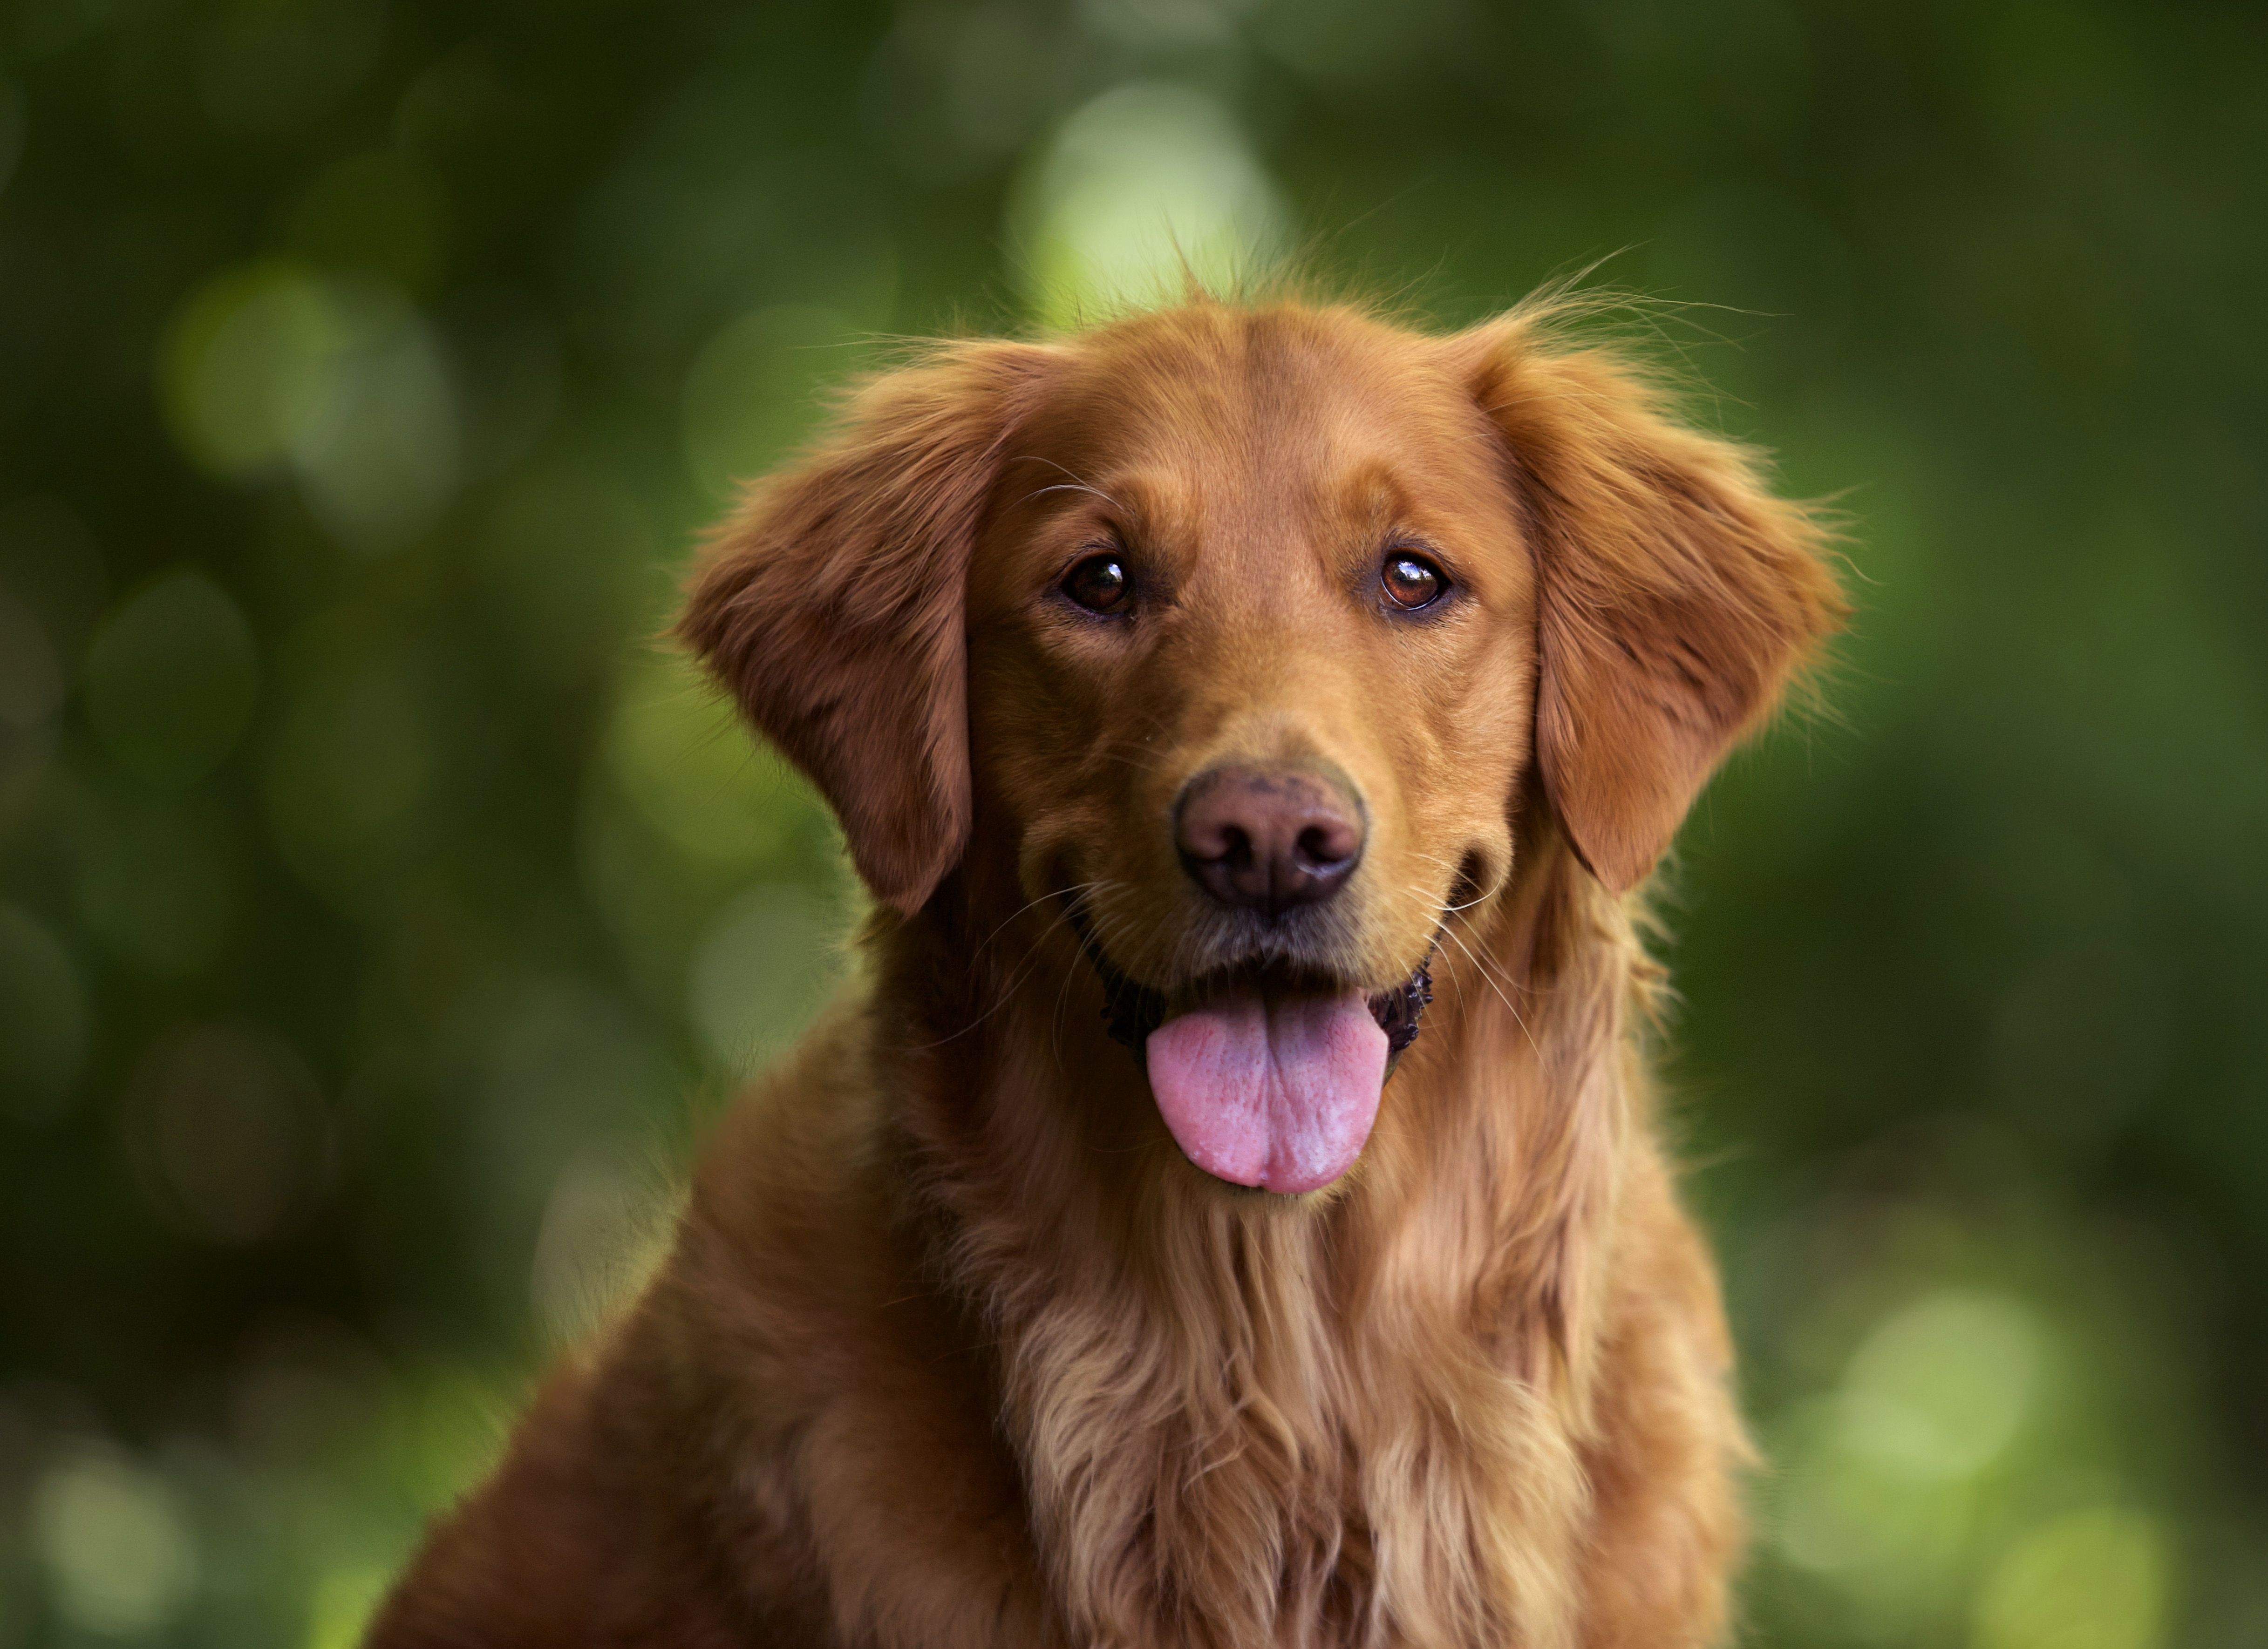
\includegraphics[width=3.5cm]{selective-focus-shot-adorable-golden-retriever-outdoors.jpg}};
        \node[above=0.2cm of img, textfont] (x_text) {$x$\\Variables observadas\\(input)};

        \node[right=2.5cm of img, labelsbox] (y_box) {
            Human \\ Animal \\ Airplane \\ Car \\ Truck
        };
        \node[above=0.2cm of y_box, textfont] (y_text) {$y$\\Variables a predecir\\(clase)};

        \node[draw, rounded corners, minimum width=8.5cm, minimum height=1.2cm,
              above=1.5cm of $(x_text.north)!0.5!(y_text.north)$,
              font=\normalsize\sffamily] (ef) {Función de Energía\quad $E_\theta(x, y)$};

        \draw[->, thick] (x_text) -- (x_text |- ef.south);
        \draw[->, thick] (y_text) -- (y_text |- ef.south);
        \draw[->, thick] (ef.north) -- ++(0, 1.2cm) coordinate (out_arrow);
        \node[right=0.1cm of out_arrow, yshift=-0.6cm, font=\small\sffamily] {};

        \begin{scope}[shift={($(ef.north)+(0, 1.3cm)$)}]
            \tikzset{bar/.style={draw, fill=gray!70, minimum height=0.2cm,
                     inner sep=0pt, anchor=west}}
            \node[left, font=\scriptsize\sffamily] at (0, 1.2) {Human};
            \node[bar, minimum width=1.5cm] at (0.1, 1.2) {};
            \node[left, font=\scriptsize\sffamily] at (0, 0.9) {Animal};
            \node[bar, minimum width=0.3cm] at (0.1, 0.9) {};
            \node[left, font=\scriptsize\sffamily] at (0, 0.6) {Airplane};
            \node[bar, minimum width=1.8cm] at (0.1, 0.6) {};
            \node[left, font=\scriptsize\sffamily] at (0, 0.3) {Car};
            \node[bar, minimum width=1.2cm] at (0.1, 0.3) {};
            \node[left, font=\scriptsize\sffamily] at (0, 0.0) {Truck};
            \node[bar, minimum width=0.9cm] at (0.1, 0.0) {};
            \draw[->, thick] (0.1, -0.2) -- (2.2, -0.2);
            \node[below, font=\scriptsize\sffamily] at (1.15, -0.2) {$E_\theta(x, y)$};
        \end{scope}
    \end{tikzpicture}
    \caption{Energía en el contexto de EBMs para una tarea de clasificación. Dada la entrada observada $x$ (imagen de un perro), el modelo evalúa la energía $E_\theta(x, y)$ para cada clase candidata $y$. La respuesta inferida es $y = \text{Animal}$, dado que tiene asociado el valor mínimo de energía de entre las posibles clases candidatas (barra más corta). Se observa, por tanto, que no requiere normalización probabilística.}
    \label{fig:ebm_inferencia_retriever}
\end{figure}

%\input{cap2_energiaBoltzmann}
\section{La Medida de Boltzmann-Gibbs y la Temperatura Inversa}
\label{sec:boltzmann_gibbs}
Para realizar inferencias probabilísticas o entrenar EBMs mediante máxima verosimilitud, es necesario transformar la función de energía $E_\theta(x, y)$ en una distribución de probabilidad condicional $p_\theta(y \mid x)$ sobre el espacio de predicción $\mathcal{Y}$. Esta correspondencia se establece a través de la \textbf{medida condicional de Boltzmann-Gibbs}:
\begin{equation}
\label{eq:boltzmann_dist}
p_\theta(y \mid x) = \frac{\exp(-\beta E_\theta(x, y))}{Z(x; \theta)}
\end{equation}
donde $\beta > 0$ es la \textbf{temperatura inversa} (o intensidad de selección, $\beta = 1/T$) que controla la dispersión del paisaje, y $Z(x; \theta)$ es la \textbf{función de partición condicional} que normaliza la medida (si $\mathcal{Y}$ es discreto, la integral se convierte en un sumatorio):

\begin{equation}
\label{eq:partition_function_cond}
Z(x; \theta) = \int_{\mathcal{Y}} \exp(-\beta E_\theta(x, y')) \, dy'
\end{equation}

El parámetro de temperatura $\beta$ modula directamente la concentración probabilística en los valles del paisaje de energía. Como ilustra la Figura \ref{fig:beta_temperature}, un valor bajo de $\beta$ (alta temperatura) suaviza la distribución haciéndola más uniforme, mientras que un valor alto de $\beta$ (baja temperatura) concentra fuertemente la masa de probabilidad condicional en los mínimos globales de energía de $\mathcal{Y}$.

\begin{figure}[htbp]
    \centering
    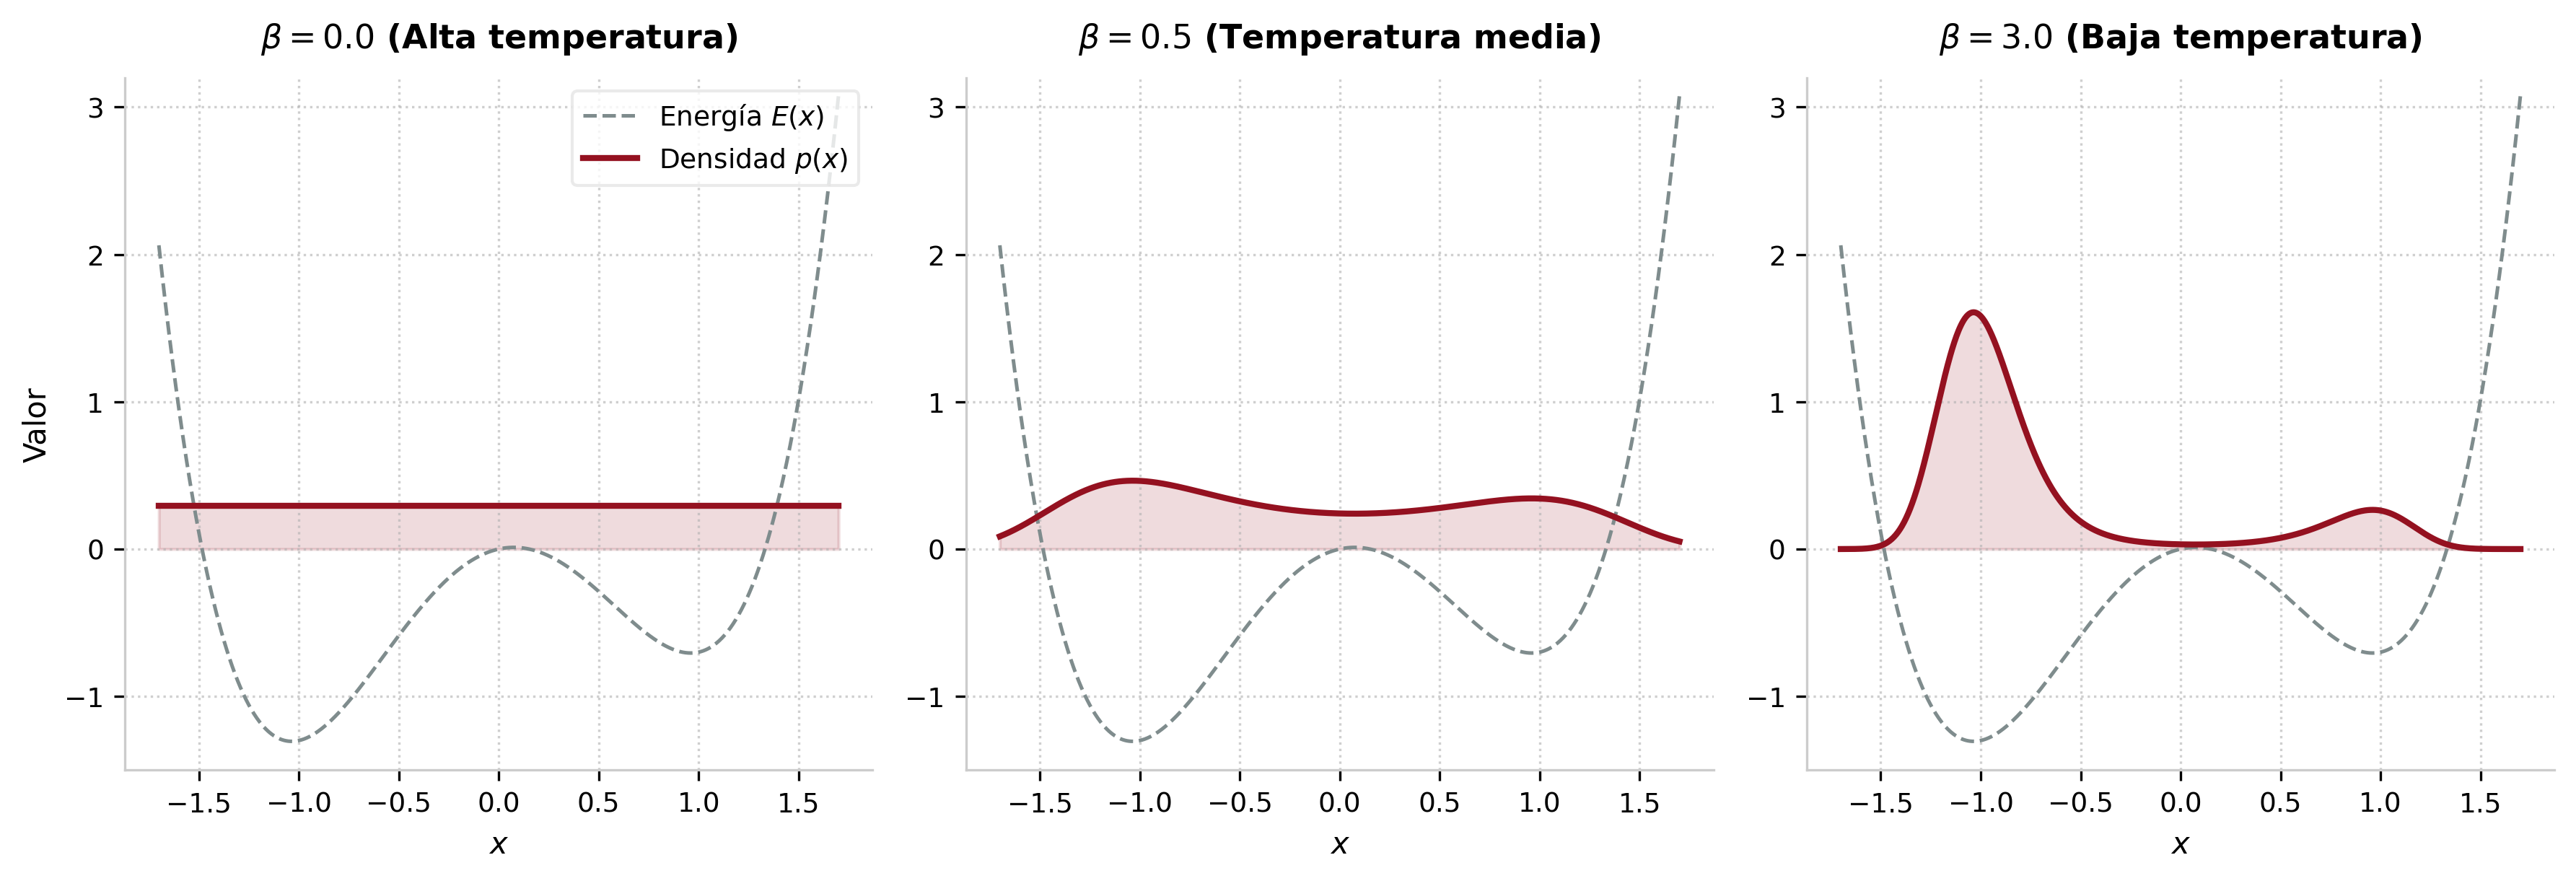
\includegraphics[width=0.95\textwidth]{beta_temperature.png}
    \caption{Evolución de la densidad de Boltzmann-Gibbs asociada a la función de energía de ejemplo $E(x) = x^4 - 2x^2 + 0.3x$, con distintos valores de $\beta$. Izquierda: $\beta = 0.0$ (alta temperatura), distribución uniforme. Centro: $\beta = 0.5$ (temperatura media), bimodalidad suave; la masa fluye con facilidad entre los valles. Derecha: $\beta = 3.0$ (baja temperatura), la masa de probabilidad se concentra fuertemente en el mínimo global de energía.}
    \label{fig:beta_temperature}
\end{figure}

\input{cap2_jaynes}

\section{El Principio de Máxima Entropía de Jaynes}
\label{sec:principio_jaynes}

La elección de la distribución condicional de Boltzmann-Gibbs de la Ecuación \eqref{eq:boltzmann_dist} puede fundamentarse en principios de teoría de la información. Es la única distribución de probabilidad que maximiza la entropía condicional sujeta a restricciones de primer momento sobre la energía.

El \textbf{Principio de Máxima Entropía de Jaynes} \cite{jaynes1957information} establece que, para una entrada fija $x \in \mathcal{X}$, la distribución de probabilidad condicional $p(y \mid x)$ que mejor representa nuestro estado de conocimiento sobre la variable de destino $y$ es aquella que \textbf{maximiza la entropía condicional de Shannon}:
\begin{equation}
\max_{p(\cdot \mid x)} \; H(p(y \mid x)) = -\sum_{y \in \mathcal{Y}} p(y \mid x) \log p(y \mid x)
\end{equation}
sujeta a las restricciones físicas impuestas por las observaciones:
\begin{align}
\text{Normalización:} \quad &\sum_{y \in \mathcal{Y}} p(y \mid x) = 1 \\
\text{Momentos de la energía:} \quad &\sum_{y \in \mathcal{Y}} p(y \mid x) f_k(x, y) = \mu_k(x), \quad \forall k=1, \dots, K
\end{align}
donde $f_k(x, y)$ son funciones de características y $\mu_k(x)$ son sus valores esperados conocidos.

La resolución analítica de este problema de optimización mediante multiplicadores de Lagrange condicionales $\lambda_k(x)$ determina de manera única que la distribución condicional de máxima entropía es:
\begin{equation}
\label{eq:solucion_jaynes}
p(y \mid x) = \frac{1}{Z(x)} \exp\left( - \sum_{k=1}^K \lambda_k(x) f_k(x, y) \right)
\end{equation}
con la función de partición $Z(x) = \sum_{y' \in \mathcal{Y}} \exp\left( - \sum_{k=1}^K \lambda_k(x) f_k(x, y') \right)$. Esta forma coincide con la distribución condicional de Boltzmann-Gibbs, donde los multiplicadores $\lambda_k(x)$ hacen el papel de la temperatura condicional inversa $\beta$.

\subsection{Conexión Adaptativa con Redes Neuronales Profundas}
\label{subsec:conexion_dnn}

La formulación de Jaynes utiliza una combinación lineal de características físicas $f_k(x, y)$ elegidas a priori:
\begin{equation}
E_{\text{Jaynes}}(x, y) = \sum_{k=1}^K \lambda_k(x) f_k(x, y)
\end{equation}
En el aprendizaje de representaciones (Representation Learning), definir manualmente estas características conjuntas para datos complejos es impracticable. Por el contrario, las Redes Neuronales Profundas resuelven esta limitación sustituyendo las funciones fijas $f_k(x, y)$ por representaciones adaptativas aprendidas de los datos.

Como se detalla en el Apéndice \ref{ap:fundamentos_dl}, una red neuronal profunda procesa la entrada conjunta $(x, y)$ a través de sus capas ocultas no lineales para calcular la energía. La salida escalar del funcional de energía $E_\theta(x, y)$ se puede interpretar en su capa de salida como una combinación lineal de las características de la última capa oculta, $\phi_k(x, y; \theta_{\text{feat}})$, ponderadas por unos pesos $w_k$ y un sesgo $b$:
\begin{equation}
E_\theta(x, y) = \sum_{k=1}^d w_k \phi_k(x, y; \theta_{\text{feat}}) + b
\end{equation}
donde $\theta = (\theta_{\text{feat}}, w, b)$ representa todos los parámetros de la red. La red neuronal no solo optimiza los multiplicadores $\lambda_k(x) = w_k$, sino que aprende de forma adaptativa las propias características $f_k(x, y)= \phi_k(x, y)$ mediante retropropagación. 

\subsection{El Dilema Probabilístico y el Salto a la Geometría}
La formulación termodinámica de Jaynes proporciona la distribución de probabilidad ideal que representa nuestro conocimiento (Máxima Entropía condicional). Sin embargo, como se detalla en la siguiente sección, el \textbf{cuello de botella computacional} de la integral de partición en espacios continuos de alta dimensión obliga a abandonar este tipo de "perfección termodinámica". 

Al prescindir de la normalización $Z$ y del "envoltorio probabilístico" $p_\theta(y \mid x)$, el modelo queda a merced de una superficie de energía \textit{no acotada probabilísticamente}. La energía pasa a interpretarse de forma puramente geométrica, computando la red, directamente un valor $E_\theta(x, y)$. Este abandono de la idea de probabilidad explica por qué en capítulos posteriores (en los que se abordan implementaciones prácticas de estos sistemas) el lenguaje de las probabilidades desaparece casi por completo en favor del álgebra lineal, la varianza y la distancia euclídea espacial.


\input{cap2_cuelloBotella}

\section{El Cuello de Botella Probabilístico: Intratabilidad de $Z(x; \theta)$}
\label{sec:cuello_botella}

Aunque la medida de Boltzmann-Gibbs condicional formaliza de manera elegante la probabilidad condicional $p_\theta(y \mid x)$ a partir de la energía $E_\theta(x, y)$, la función de partición condicional $Z(x; \theta)$ representa un cuello de botella computacional en espacios continuos de alta dimensión.

\subsection{Escenario Discreto vs. Continuo}
En espacios discretos finitos $\mathcal{Y} = \{y_1, \dots, y_K\}$ (como el vocabulario de un LLM), la función de partición se reduce a una suma finita:
\begin{equation}
Z(x; \theta) = \sum_{k=1}^K e^{-\beta E_\theta(x, y_k)}
\end{equation}
La aplicación de la normalización sobre esta suma es el operador \textbf{Softmax}, que es relativamente fácil en dominios discretos. Por el contrario, en dominios continuos como imágenes o vídeos $\mathcal{Y} \subseteq \mathbb{R}^D$, la dimensión del espacio (el número de píxeles o variables continuas) puede, fácilmente, llegar a ser del orden de $D \approx 10^6$. Es crucial distinguir esta dimensionalidad del número total de configuraciones posibles: incluso si discretizáramos cada variable en solo $256$ niveles de intensidad, la cardinalidad del espacio de búsqueda sería de $256^D \approx 10^{2.4 \times 10^6}$ combinaciones, un valor que supera por órdenes de magnitud al número de átomos del universo observable (estimado tradicionalmente en $\sim 10^{80}$). En este caso, la función de partición viene dada por la integral de Lebesgue:
\begin{equation}
Z(x; \theta) = \int_{\mathcal{Y}} e^{-\beta E_\theta(x, y')} \, dy'
\end{equation}
Esta integral carece de solución analítica para funciones de energía no lineales modeladas por redes neuronales. Además, cualquier aproximación numérica directa (como la cuadratura) es inviable debido a la maldición de la dimensionalidad (\textit{curse of dimensionality}), ya que el número de puntos de evaluación crece exponencialmente con $D$.

\subsection{El Gradiente de la Log-Partición y MCMC}
Al trabajar con funciones de verosimilitud, la intractabilidad del término de normalización $Z(x; \theta)$ se propaga al cálculo del gradiente de la log-verosimilitud. Dado que el entrenamiento de redes neuronales se basan en descenso por gradiente (Apéndice~\ref{sec:backprop}), esta intractabilidad obstaculiza este proceso de optimización. El gradiente de la función de partición logarítmica respecto a los parámetros $\theta$ se obtiene como:
\begin{align}
\nabla_\theta \log Z(x; \theta) &= \frac{1}{Z(x; \theta)} \nabla_\theta \int_{\mathcal{Y}} e^{-\beta E_\theta(x, y')} \, dy' \nonumber \\
&= -\beta \int_{\mathcal{Y}} \frac{e^{-\beta E_\theta(x, y')}}{Z(x; \theta)} \nabla_\theta E_\theta(x, y') \, dy' \nonumber \\
&= -\beta \, \mathbb{E}_{p_\theta(y \mid x)} \left[ \nabla_\theta E_\theta(x, y) \right]
\end{align}

Evaluar este gradiente exige calcular la esperanza matemática bajo la propia distribución del modelo $p_\theta(y \mid x)$. Dado que no podemos evaluar $Z(x; \theta)$, no podemos muestrear de $p_\theta$ directamente y se debe recurrir a algoritmos de Monte Carlo por Cadenas de Markov (MCMC), como las dinámicas de Langevin. En escenarios realistas de dimensiones de píxeles, MCMC es prohibitivo debido a:
\begin{itemize}
    \item \textbf{Lentitud de convergencia:} Requiere ejecutar cientos de pasos de inferencia de la red neuronal para cada muestra individual durante el bucle de optimización.
    \item \textbf{Mode Mixing:} La densidad condicional de imágenes reales es altamente multimodal. Las MCMC quedan atrapadas en mínimos locales de energía y son incapaces de transitar entre modos distantes, sesgando el gradiente del estimador.
\end{itemize}

Esta barrera  motiva el abandono del paradigma probabilístico: las JEA prescinden por completo de la normalización probabilística y de $Z(x; \theta)$, operando de forma no normalizada en el espacio latente.


\input{cap2_ebmSSL}

\section{EBMs como Marco para el Aprendizaje de Compatibilidades (SSL)}
\label{sec:ebm_ssl}

En el Aprendizaje Auto-Supervisado (SSL), el objetivo no es clasificar o predecir etiquetas, sino capturar la estructura intrínseca de los datos a partir de relaciones de consistencia. En este contexto, los EBMs se formulan sobre el espacio conjunto $\mathcal{X} \times \mathcal{Y}$ para evaluar la compatibilidad mutua de variables mediante la función de energía $E_\theta(x, y)$. Un valor de energía bajo $E_\theta(x, y)$ indica que el par de variables es consistente o compatible, mientras que un valor alto representa incompatibilidad. Este marco de compatibilidad se adapta de forma natural a las \textit{pretext tasks} (tareas auxiliares diseñadas para extraer información de supervisión de los propios datos) de SSL.

\begin{enumerate}
    \item \textbf{Predicción de regiones ocultas (Inpainting):} Sea $x_o \in \mathcal{X}_o$ la porción observada de una imagen y $x_h \in \mathcal{X}_h$ la región oculta a predecir. El EBM aprende una función de energía $E_\theta(x_o, x_h)$ que toma valores mínimos únicamente cuando la porción $x_h$ es una continuación visualmente coherente de $x_o$.
    
    \begin{figure}[htbp]
        \centering
        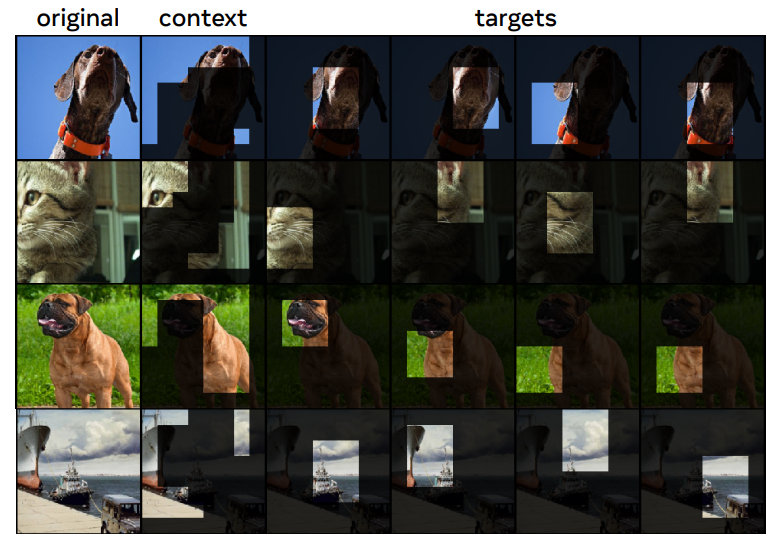
\includegraphics[width=0.8\textwidth]{SSL_inpainting.png}
        \caption{Representación de la predicción de regiones ocultas. La porción observada $x_o$ (contexto) y la porción real oculta $x_h$ (target) forman un par de baja energía $E_\theta(x_o, x_h)$, mientras que parches incorrectos elevan la energía.}
        \label{fig:ssl_inpainting}
    \end{figure}
    
    \item \textbf{Consistencia entre vistas aumentadas:} Dadas dos transformaciones aumentadas de una misma muestra $x$, denotadas como $x_1 = T_1(x)$ y $x_2 = T_2(x)$, el modelo evalúa su compatibilidad mediante $E_\theta(x_1, x_2)$. El EBM se optimiza para asignar energías bajas a las vistas que proceden de la misma muestra de origen y energías altas a vistas procedentes de muestras distintas.
\end{enumerate}

\subsection{Modelado de Compatibilidad sin Densidades de Probabilidad}
El éxito de los EBMs en SSL reside en que modelan la compatibilidad de forma directa mediante la función de energía no normalizada $E_\theta(x, y)$, evitando estimar densidades condicionales normalizadas $p_\theta(y \mid x)$. Al prescindir de la normalización, se esquiva por completo la intratabilidad del cálculo de la función de partición condicional $Z(x; \theta)$ en espacios de alta dimensión continuo como los píxeles (Sección \ref{sec:cuello_botella}).

\subsection{Las JEA como EBMs No Probabilísticos}
\label{subsec:jeas_como_ebm}

El paradigma de las \textbf{Joint Embedding Architectures (JEA)} es una realización concreta de los EBMs no probabilísticos en el espacio latente. En lugar de evaluar la compatibilidad de las entradas en el espacio físico de píxeles $\mathbb{R}^D$, las JEA proyectan $x$ e $y$ a un espacio latente de baja dimensión $\mathcal{Z} \subseteq \mathbb{R}^d$ ($d \ll D$) utilizando dos codificadores (encoders) $f_\theta$ y $g_\phi$.

Se define la \textbf{función de energía de la JEA} como la distancia euclídea al cuadrado entre los embeddings latentes de ambas variables:
\begin{equation}
\label{eq:energia_jea_latente}
E_{\theta, \phi}(x, y) = \mathcal{L}_{\text{JEA}}(x, y) = \| f_\theta(x) - g_\phi(y) \|_2^2
\end{equation}

Esta formulación aporta tres ventajas cruciales:
\begin{enumerate}
    \item \textbf{Se evita la reconstrucción:} La compatibilidad es medida directamente en $\mathcal{Z}$. Los encoders actúan como filtros de información que descartan el ruido estocástico de alta frecuencia (como detalles de fondo) y retiene únicamente características semánticas robustas.
    \item \textbf{Ausencia de normalización:} La ecuación \eqref{eq:energia_jea_latente} es estrictamente no normalizada. Evita computar la función de partición condicional $Z(x; \theta)$ sobre imágenes continuas, solucionando el cuello de botella predictivo de la integral de Lebesgue en $\mathbb{R}^D$.
    \item \textbf{Geometrización semántica:} La superficie de energía se define por la métrica de $\mathcal{Z}$. Minimizar la energía acerca las representaciones latentes de muestras coherentes, estructurando la geometría del espacio de embeddings.
\end{enumerate}

Como se detalla en el Capítulo~\ref{cap:siamesas_colapso}, la gran limitación de este enfoque no probabilístico es que, al carecer de normalización condicional o muestras negativas, el sistema tiende de forma natural al \textbf{colapso de representación}: una solución degenerada donde los encoders se vuelven constantes ($f_\theta(x) = g_\phi(y) = c$), minimizando la energía a cero de forma trivial sin extraer ninguna información semántica de la realidad.
\chapter{Orígenes de Joint Embedding: Redes Siamesas y el Colapso de Representación}
\label{cap:siamesas_colapso}

La idea de comparar representaciones en lugar de reconstruir entradas físicas se remonta a principios de los 90, con la introducción de las redes siamesas. Sin embargo, este paradigma no tardó en toparse con un obstáculo fundamental: el Representation Collapse (o Colapso de Representación). En este capítulo se analizan formalmente las redes siamesas y se deducen matemáticamente las causas de este colapso.

\section{Las Redes Siamesas de Bromley (1993)}
\label{sec:siamesas_bromley}

Las redes siamesas fueron concebidas por Jane Bromley y Yann LeCun en Bell Labs \cite{bromley1993signature} para resolver el problema práctico de la verificación de firmas manuscritas. La idea central es construir un encoder que proyecte datos pertenecientes a una misma persona (misma clase semántica) a puntos cercanos en el espacio de embeddings $\mathcal{Z}$, y firmas de distintas personas (o firmas fraudulentas) a puntos distantes.

\begin{definition}[Arquitectura de Red Siamesa]
Sea $\mathcal{X} \subseteq \mathbb{R}^D$ el espacio de imágenes de entrada. Consideremos un único modelo de red neuronal parametrizado por un vector de pesos $W \in \mathbb{R}^M$, que define una función diferenciable $f_W: \mathbb{R}^D \to \mathbb{R}^d$. 
La arquitectura siamesa consta de dos copias idénticas de esta función (que comparten exactamente el mismo vector de parámetros $W$). Dadas dos entradas $x_1, x_2 \in \mathcal{X}$, la red calcula sus embeddings en paralelo:
\begin{equation}
z_1 = f_W(x_1), \quad z_2 = f_W(x_2)
\end{equation}

La métrica de distancia en el espacio latente se define mediante la distancia euclídea:
\begin{equation}
d_W(x_1, x_2) = \| f_W(x_1) - f_W(x_2) \|_2
\end{equation}
\end{definition}

Aunque la distancia euclídea $d_W$ mide la disimilitud geométrica, en la formulación de la pérdida suele emplearse su cuadrado, conocido como error cuadrático medio, para garantizar la diferenciabilidad del gradiente (distancia cuadrática, Sección~\ref{sec:loss_functions} del Apéndice~\ref{ap:fundamentos_dl}). Esta estructura de pesos compartidos garantiza que dos entradas idénticas $x_1 = x_2$ se proyecten obligatoriamente en el mismo punto del espacio $\mathcal{Z}$ $z_1 = z_2$, preservando la reflexividad de la distancia.

\section{Representation Collapse}
\label{sec:demostracion_colapso}

El colapso de representación ocurre cuando la red encuentra una solución trivial que minimiza la distancia $d_W$ entre muestras similares sin extraer características útiles de los datos.

\begin{remark}[Notación Poblacional]
\label{subsec:enfoque_probabilistico}
Esta sección se constituye desde un enfoque teórico, por tanto, a menudo se sustituirán los estimadores empíricos sobre \textit{minibatches} por sus versiones poblacionales; por ejemplo, el promedio se sustituirá por la esperanza matemática ($\mathbb{E}$) sobre la verdadera distribución de los datos ($p_{\text{pos}}$ y $p_{\text{data}}$). Aunque el entrenamiento en la práctica se realiza sobre conjuntos finitos, este enfoque permite analizar con mayor rigor las causas del colapso, eliminando el ruido y las limitaciones del muestreo empírico.
\end{remark}

\subsection{El Colapso Constante como Mínimo Global}
\label{subsec:colapso_constante}



Consideremos un escenario de entrenamiento donde únicamente disponemos de un conjunto empírico de pares compatibles (también llamados pares positivos) $\mathcal{D} = \{(x_1^{(i)}, x_2^{(i)})\}_{i=1}^N$. Estos pares representan casos compatibles, por ejemplo varias vistas de un mismo objeto o, en el caso de las redes siamesas originales, dos firmas de la misma persona. En la práctica, el objetivo de la red es minimizar el promedio de las distancias cuadráticas sobre este conjunto o sobre minibatches (Apéndice~\ref{subsec:minibatch}):

\begin{equation}
\hat{\mathcal{L}}_{\text{pos}}(W) = \frac{1}{N} \sum_{i=1}^N \| f_W(x_1^{(i)}) - f_W(x_2^{(i)}) \|_2^2
\label{eq:L_pos_empirica}
\end{equation}

Sin embargo, asumiendo que los pares provienen de una distribución conjunta $p_{\text{pos}}(x_1, x_2)$ sobre $\mathcal{X} \times \mathcal{X}$, el verdadero propósito es optimizar el modelo sobre toda la población de datos subyacente. Por ello, el análisis teórico requiere abstraerse del sumatorio empírico y definir la función de pérdida global como la esperanza matemática de la distancia cuadrática:

\begin{equation}
\mathcal{L}_{\text{pos}}(W) = \mathbb{E}_{(x_1, x_2) \sim p_{\text{pos}}} \left[ \| f_W(x_1) - f_W(x_2) \|_2^2 \right]
\label{eq:L_pos}
\end{equation}

Esta formulación basada en la esperanza y no en el estimador empírico es el estándar adoptado en la literatura \cite{wang2020understanding}. A partir de este objetivo poblacional, podemos demostrar que el colapso a constante es un mínimo global y un atractor estable del gradiente para esta función de pérdida.

\begin{figure}[H]
\centering
\begin{tikzpicture}[node distance=1.5cm, auto, >=Stealth]
    % Entradas con las imágenes de las firmas
    \node (x1) [draw, rectangle, minimum width=2.5cm, minimum height=1.5cm] {
\includegraphics[width=2.3cm, height=1.3cm]{signature_Rodlf1.png}};
    \node (x2) [draw, rectangle, minimum width=2.5cm, minimum height=1.5cm, below=of x1, yshift=-0.5cm] {
\includegraphics[width=2.3cm, height=1.3cm]{signature_Rodlf2.png}};
    
    % Textos descriptivos de las entradas
    \node [above=0.05cm of x1, font=\footnotesize] {Entrada $x_1$ (Firma A)};
    \node [below=0.05cm of x2, font=\footnotesize] {Entrada $x_2$ (Firma B)};
    
    % Encoders siameses (comparten W)
    \node (f1) [draw, rectangle, minimum width=2cm, minimum height=1cm, right=of x1, xshift=1cm] {Encoder $f_{W}$};
    \node (f2) [draw, rectangle, minimum width=2cm, minimum height=1cm, right=of x2, xshift=1cm] {Encoder $f_{W}$};
    
    % Espacio latente colapsado (z1 = z2 = c)
    \node (z) [circle, draw, double, red, thick, minimum size=1.5cm] at ($(f1.east)!0.5!(f2.east) + (2.5cm,0)$) {$z_1 = z_2 = c$};
    \node [above=0.1cm of z, font=\footnotesize\bfseries, align=center, red] {Espacio Latente $\mathcal{Z}$\\};
    
    % Pérdida (Loss)
    \node (loss) [draw, diamond, minimum width=1.5cm, minimum height=1.5cm, right=of z, xshift=0cm] {Loss = 0}; 

    % Conexiones
    \draw[->] (x1) -- (f1);
    \draw[->] (x2) -- (f2);
    \draw[->] (f1.east) -- (z.north west);
    \draw[->] (f2.east) -- (z.south west);
    \draw[->] (z) -- (loss);
    \draw[dashed, <->] (f1) -- node[left] {Shared $W$} (f2);
\end{tikzpicture}
\caption{Ilustración del colapso de representación constante en una arquitectura siamesa con firmas manuscritas. Dos entradas diferentes $x_1$ y $x_2$ correspondientes a firmas de la misma persona se proyectan por encoders idénticos $f_W$ a un único punto constante $c$ en el espacio latente $\mathcal{Z}$. Aunque este mapeo trivial minimiza la distancia $d_W(x_1, x_2)$ resultando una pérdida de cero, la representación resultante carece de valor al eliminar toda variación semántica.}
\label{fig:colapso_siamesas}
\end{figure}

\begin{theorem}[Colapso de Representación Constante]
Cualquier mapeo constante de la forma $f_{W^*}(x) = c$ para todo $x \in \mathcal{X}$, donde $c \in \mathbb{R}^d$ es un vector constante arbitrario, es un mínimo global absoluto de la función de pérdida $\mathcal{L}_{\text{pos}}(W)$.
\end{theorem}

\begin{proof}
Dado que la norma euclídea al cuadrado es no negativa por definición, tenemos que:
\begin{equation}
\| f_W(x_1) - f_W(x_2) \|_2^2 \ge 0 \quad \forall x_1, x_2 \in \mathcal{X}
\end{equation}
Tomando la esperanza matemática en ambos lados de la desigualdad, se deduce directamente que la función de pérdida está acotada inferiormente por cero:
\begin{equation}
\mathcal{L}_{\text{pos}}(W) \ge 0 \quad \forall W \in \mathbb{R}^M
\end{equation}
Evaluamos ahora la función de pérdida para el mapeo constante $f_{W^*}(x) = c$:
\begin{equation}
\mathcal{L}_{\text{pos}}(W^*) = \mathbb{E}_{(x_1, x_2) \sim p_{\text{pos}}} \left[ \| c - c \|_2^2 \right] = \mathbb{E}_{(x_1, x_2)} [ 0 ] = 0
\end{equation}
Dado que la pérdida alcanza su cota inferior global absoluta en $W^*$, el mapeo constante $f_{W^*}(x) = c$ es un mínimo global de $\mathcal{L}_{\text{pos}}(W)$.
\end{proof}


El teorema establece la existencia del colapso como mínimo global, pero no dice nada 
sobre si el descenso de gradiente converge efectivamente hacia él. Analicemos la dinámica de optimización mediante descenso de gradiente. 

Sea $\theta_k \in W$ un parámetro individual de la red. Aplicando la regla de la cadena bajo la integral (regla de Leibniz), la derivada parcial de la pérdida respecto a $\theta_k$ es:

\begin{equation}
\frac{\partial \mathcal{L}_{\text{pos}}(W)}{\partial \theta_k} = \mathbb{E}_{(x_1, x_2) \sim p_{\text{pos}}} \left[ 2 \left( f_W(x_1) - f_W(x_2) \right)^T \left( \frac{\partial f_W(x_1)}{\partial \theta_k} - \frac{\partial f_W(x_2)}{\partial \theta_k} \right) \right]
\end{equation}

En el estado colapsado $f_{W^*}(x) = c$, el factor de diferencia se anula para cualquier par:
\begin{equation}
f_{W^*}(x_1) - f_{W^*}(x_2) = c - c = \vec{0} \quad \forall\, x_1, x_2 \in \mathcal{X}
\end{equation}

Sustituyendo en la expresión del gradiente:
\begin{equation}
\frac{\partial \mathcal{L}_{\text{pos}}(W^*)}{\partial \theta_k} = \mathbb{E}_{(x_1, x_2) \sim p_{\text{pos}}} \left[ 2 \cdot \vec{0}^{\,T} \left( \frac{\partial f_W(x_1)}{\partial \theta_k} - \frac{\partial f_W(x_2)}{\partial \theta_k} \right) \right] = 0
\end{equation}

El gradiente se anula idénticamente para todo $\theta_k$, de modo que las iteraciones del descenso quedan detenidas: $W^{(t+1)} = W^{(t)} - \eta \nabla_W \mathcal{L}_{\text{pos}}(W^{(t)}) = W^{(t)}$. El estado colapsado es, por tanto, un punto fijo del optimizador.

Que sea además un \emph{atractor} se sigue de la estructura de la pérdida $\mathcal{L}_{\text{pos}}$, que únicamente penaliza la distancia entre representaciones de pares positivos, sin disponer de fuerzas contrapuesta que obligue a dispersar los embeddings. Cada paso de optimización reduce progresivamente esa distancia, contrayendo las representaciones hacia un mismo punto. 

Esta dinámica se acentúa cuando la red se inicializa cerca del colapso (p.e. con pesos pequeños) que producen embeddings casi idénticos. En ese régimen, $f_W(x_1) - f_W(x_2) \approx \vec{0}$ hace que el gradiente sea ya casi nulo, eliminando cualquier señal que pudiera diversificar las representaciones. La única dirección de actualización disponible sigue siendo contractiva, 
de modo que el optimizador no dispone de señal para escapar hacia 
representaciones más diversas. En ausencia de mecanismos que penalicen 
la contracción, esta dinámica favorece la convergencia hacia el colapso total, 
aunque el resultado depende en general de la inicialización y de la 
estructura de los datos.


\section{Colapso Dimensional}
\label{sec:colapso_dimensional_v2}

Se distinguen dos formas de degeneración geométrica en el espacio de representación. El colapso total o trivial es aquel donde el encoder contrae toda la variedad de entrada a un único punto invariante. Por el contrario, el \emph{colapso dimensional} es una patología más sutil: las representaciones escapan del punto trivial pero quedan confinadas en un subespacio propio de menor dimensión, perdiendo capacidad expresiva de forma irreversible.

\begin{definition}[Colapso Dimensional]
Sea $\mathcal{X}$ el espacio de entrada y $f_W: \mathcal{X} \to \mathbb{R}^d$ un encoder parametrizado por los pesos $W$, donde $d$ representa la dimensionalidad de salida. Aunque la pérdida de la red se optimiza midiendo distancias sobre pares compatibles ($p_{\text{pos}}$), la riqueza o expresividad del espacio latente se evalúa comprobando la diversidad de todas las imágenes de forma global. Por ello, definimos formalmente la matriz de covarianza del espacio de representaciones evaluando la esperanza sobre la distribución $p_{\text{data}}$ (Apéndice~\ref{sec:al_covarianza_rango}):
\begin{equation}
    \Sigma_\mathcal{Z} = \mathbb{E}_{x \sim p_{\text{data}}}\left[(f_W(x) - \mu)(f_W(x) - \mu)^T\right] \in \mathbb{R}^{d \times d}
\end{equation}
donde $\mu = \mathbb{E}_{x \sim p_{\text{data}}}[f_W(x)] \in \mathbb{R}^d$ es el vector de medias del espacio $\mathcal{Z}$. Decimos que la representación sufre colapso dimensional si:
\begin{equation}
    \operatorname{rango}(\Sigma_\mathcal{Z}) = r < d.
\end{equation}
\end{definition}

\begin{remark}[Suficiencia muestral y rango empírico]
En el escenario empírico sobre un batch de tamaño $B$, se usa el estimador $\hat{\Sigma}_\mathcal{Z} = \frac{1}{B-1}(Z - \bar{Z})^T(Z - \bar{Z})$, donde $Z \in \mathbb{R}^{B \times d}$. Recordemos que si $B \le d$, la matriz es singular. El colapso dimensional es una propiedad asintótica o poblacional donde incluso si $B \gg d$, $\operatorname{rango}(\Sigma_\mathcal{Z}) = r < d$.
\end{remark}

 Usaremos el Teorema Espectral para Matrices Simétricas (Apéndice~\ref{sec:al_teorema_espectral}). Dado que $\Sigma_\mathcal{Z}$ es simétrica y semidefinida positiva, existe una base ortonormal de $\mathbb{R}^d$ formada por autovectores de $\Sigma_\mathcal{Z}$. Podemos descomponerla diagonalmente como:
\begin{equation}
    \Sigma_\mathcal{Z} = Q \Lambda Q^T = 
    \begin{pmatrix}
        | & & | \\
        q_1 & \dots & q_d \\
        | & & |
    \end{pmatrix}
    \begin{pmatrix}
        \sigma_1^2 & & & 0 \\
        & \ddots & & \\
        & & \sigma_r^2 & \\
        0 & & & \mathbf{0}_{d-r}
    \end{pmatrix}
    \begin{pmatrix}
        - & q_1^T & - \\
          & \vdots &   \\
        - & q_d^T & -
    \end{pmatrix}
\end{equation}
donde $\sigma_1^2 \ge \dots \ge \sigma_r^2 > 0$ representan la varianza de los datos a lo largo de las direcciones principales $q_i$. Por el \textbf{Teorema de la Dimensión} (Apéndice~\ref{ap:algebra_lineal}):
\begin{equation}
    \dim(\operatorname{Ker}(\Sigma_\mathcal{Z})) = d - \operatorname{rango}(\Sigma_\mathcal{Z}) = d - r.
\end{equation}
Cualquier vector $v \in \operatorname{Ker}(\Sigma_\mathcal{Z}) \subseteq \mathbb{R}^d$ constituye una dirección de colapso donde la varianza es nula. Esto significa que el encoder concentra las representaciones de los datos sobre el subespacio afín $f_W(x) \in \mu + (\operatorname{Ker}(\Sigma_\mathcal{Z}))^\perp$ para casi todo $x \sim p_{\text{data}}.$ En términos geométricos, al carecer de varianza, a lo largo de las direcciones del núcleo los datos no se desvían de su media $\mu$ colapsando esas dimensiones a constante.

\begin{proposition}[Estabilidad del Colapso Dimensional]
Sea $f_W$ un encoder parametrizado por $W$ y sea $W^*$ un estado de la red donde $\operatorname{rango}(\Sigma_\mathcal{Z}) = r < d$. Para todo vector del núcleo $v \in \operatorname{Ker}(\Sigma_\mathcal{Z}) \subseteq \mathbb{R}^d$, la varianza de las proyecciones sobre $v$ es nula, es decir, $v^T f_{W^*}(x)$ es constante para casi todo $x \sim p_{\text{data}}.$ 

Dado que las distribuciones marginales de los pares en $p_{\text{pos}}$ coinciden exactamente con $p_{\text{data}}$ (cada elemento del par es una muestra de la distribución real), se cumple que $v^T(f_{W^*}(x) - f_{W^*}(x^+)) = 0$ para casi todo $(x, x^+) \sim p_{\text{pos}}$, y por la regla de la cadena, la componente de cualquier gradiente derivado de la pérdida positiva $\mathcal{L}_{\text{pos}}$ que intente actualizar las representaciones en la dirección $v$ es idénticamente nula. Por tanto, el subespacio nulo es un invariante algebraico bajo la dinámica de optimización:
\begin{equation}
    v^T \nabla_{f_W} \mathcal{L}_{\text{pos}}(W^*) = 0.
\end{equation}
\end{proposition}

\subsection*{Mecanismo Dinámico: El Flujo de Gradiente como Operador de Contracción}

La proposición anterior ilustra de manera general por qué el colapso es un estado absorbente, pero no explica el proceso dinámico mediante el cual el sistema precipita hacia él. Siguiendo el marco analítico establecido por Jing et al.~\cite{jing2022understanding} para el estudio del flujo de gradiente en redes siamesas, descompondremos el factor lineal de la capa final $f_W(x) = W\phi(x)$ (Apéndice~\ref{subsec:capa_proyeccion}), con pesos $W \in \mathbb{R}^{d \times m}$ y siendo $\phi(x) \in \mathbb{R}^{m}$ la salida de la capa $L-1$ (siendo $L$ el número de capas).

\begin{figure}[H]
\centering
\begin{tikzpicture}[node distance=0.8cm, auto, >=Stealth]
    % Nodos de la arquitectura
    \node (x) [draw, rectangle, rounded corners, minimum width=1.2cm, minimum height=1cm, fill=gray!10, font=\footnotesize] {Entrada $x$};
    
    \node (encoder) [draw, rectangle, minimum width=2.4cm, minimum height=1.2cm, right=of x, fill=blue!5, align=center, font=\footnotesize] {Encoder no lineal\\(Capas $1$ a $L-1$)};
    
    \node (phi) [draw, circle, inner sep=1pt, minimum size=0.9cm, right=of encoder, fill=green!5, font=\footnotesize] {$\phi(x)$};
    \node [above=0.1cm of phi, font=\scriptsize, align=center] {Pre-activ.\\$\mathbb{R}^m$};
    
    \node (W) [draw, rectangle, minimum width=1.8cm, minimum height=1.2cm, right=of phi, fill=orange!5, align=center, font=\footnotesize] {Proyección\\Lineal $W$};
    
    \node (f) [draw, circle, double, inner sep=1pt, minimum size=0.9cm, right=of W, fill=red!5, font=\footnotesize] {$f_W(x)$};
    \node [above=0.1cm of f, font=\scriptsize, align=center] {Espacio lat.\\$\mathbb{R}^d$};

    % Flechas de flujo de datos
    \draw[->, thick] (x) -- (encoder);
    \draw[->, thick] (encoder) -- (phi);
    \draw[->, thick] (phi) -- (W);
    \draw[->, thick] (W) -- (f);
    
    % Caja general agrupando todo
    \draw[dashed, gray] ($(encoder.north west)+(-0.2,0.8)$) rectangle ($(W.south east)+(0.2,-0.4)$);
    \node[gray, font=\footnotesize] at ($(encoder.north)!0.5!(W.north) + (0, 1.1)$) {Red Neuronal Completa $f_W$};
\end{tikzpicture}
\caption{Descomposición estructural de la red neuronal para el análisis del colapso. El procesamiento de la entrada $x$ se divide en un extractor de características complejo (que engloba todas las transformaciones no lineales hasta la capa $L-1$) generando el vector $\phi(x)$, seguido de un operador puramente lineal parametrizado por la matriz $W$ que proyecta estas representaciones al espacio final.}
\label{fig:descomposicion_lineal}
\end{figure}
El objetivo de este análisis es mostrar formalmente que la pérdida $\mathcal{L}_{\text{pos}}$ actúa como un \textbf{operador contractivo} que empuja la red hacia el colapso dimensional. Para evidenciar matemáticamente esta fuerza de contracción, es indispensable separar la contribución de los parámetros $W$, de la estructura geométrica intrínseca de los datos.

Para ello, recordemos la forma general de la pérdida que queda como:
\begin{equation}
    \mathcal{L}_{\text{pos}}(W) = \mathbb{E}_{p_{\text{pos}}} \left[ \| W\phi(x) - W\phi(x^+) \|_2^2 \right].
\end{equation}

A partir de aquí, podemos reescribir la función de pérdida de forma cuadrática añadiendo el factor $\frac{1}{2}$, habitual en optimización para cancelar el exponente al derivar. Sea $\Delta \phi = \phi(x) - \phi(x^+)$ por tanto:

\begin{equation}
    \mathcal{L}_{\text{pos}}(W) = \frac{1}{2}\mathbb{E}_{p_{\text{pos}}} \left[\|W \Delta \phi\|_2^2 \right].
\end{equation}

Aplicando las propiedades: $v^T v = \|v\|_2^2 $, $v^T v = \operatorname{Tr}(v v^T)$ y $\operatorname{Tr}(AB) = \operatorname{Tr}(BA)$:

\begin{equation}
    \|W \Delta \phi\|_2^2 = \operatorname{Tr}\left( (W \Delta \phi) (W \Delta \phi)^T \right) = \operatorname{Tr}\left( W (\Delta \phi \Delta \phi^T) W^T \right).
\end{equation}

Sustituyendo lo anterior y aplicando linealidad de la esperanza:
\begin{equation}
    \mathcal{L}_{\text{pos}}(W) = \frac{1}{2} \mathbb{E}_{p_{\text{pos}}}\left[ \| W \Delta \phi \|_2^2 \right] = \frac{1}{2} \operatorname{Tr}\left( W \mathbb{E}_{p_{\text{pos}}}\left[ \Delta \phi \Delta \phi^T \right] W^T \right).
\end{equation}

Definimos ahora la matriz de covarianza diferencial en la capa $L-1$ como:
\begin{equation}
    \Sigma_{\Delta} = \mathbb{E}_{p_{\text{pos}}}\left[(\phi(x) - \phi(x^+))(\phi(x) - \phi(x^+))^T\right] \in \mathbb{R}^{m \times m}.
\end{equation}

Sustituyendo esta definición, la pérdida se expresa como forma cuadrática: 

\begin{equation}
    \mathcal{L}_{\text{pos}}(W) = \frac{1}{2} \operatorname{Tr}\left( W \Sigma_{\Delta} W^T \right).
\end{equation}
\vspace{10pt}

Para estudiar la dinámica del descenso de gradiente resulta conveniente considerar el sistema dinámico continuo asociado, conocido como Gradient Flow (Apéndice~\ref{sec:al_flujo_gradiente}):

\begin{equation}
    \dot{W}(t) = -\nabla_W \mathcal{L}_{\text{pos}}(W(t)).
\end{equation}

Como $\mathcal{L}_{\text{pos}}$ es una forma cuadrática, $-\nabla_W \mathcal{L}_{\text{pos}}(W(t))= -W(t) \Sigma_{\Delta}$ y por tanto:

\begin{equation}
    \dot{W}(t) = -W(t) \Sigma_{\Delta}.
\end{equation}

A continuación, resolvemos el sistema para estudiar su convergencia. Siguiendo a Jing et al.~\cite{jing2022understanding}, asumimos que la matriz de covarianza diferencial $\Sigma_{\Delta}$ es constante en el tiempo, lo que permite obtener una solución analítica cerrada.

Dado que $\Sigma_{\Delta}$ está definida como la esperanza de un producto, es por construcción una matriz \textbf{semi-definida positiva}. Aplicando el Teorema Espectral, descomponemos la matriz $\Sigma_{\Delta} = U \Lambda_{\Delta} U^T$, donde $U \in \mathbb{R}^{m \times m}$ es una matriz ortogonal ($U^T U = I$) y $\Lambda_{\Delta} = \operatorname{diag}(\lambda_1, \dots, \lambda_m)$ contiene sus autovalores. Debido a que la matriz es semi-definida positiva, se garantiza matemáticamente que todos sus autovalores son no negativos ($\lambda_j \ge 0$), representando la magnitud de la varianza de los cambios a lo largo de cada dirección geométrica principal. Introducimos el cambio de variables

\begin{equation}
    \tilde{W}(t) = W(t)U.
\end{equation}

Multiplicando la ecuación diferencial por la derecha por $U$ y utilizando que
$\Sigma_{\Delta}U = U\Lambda_{\Delta}$, obtenemos:

\begin{equation}
    \dot{W}(t)U
    = -W(t)\Sigma_{\Delta}U
    = -W(t)U\Lambda_{\Delta}.
\end{equation}

Por definición de $\tilde{W}(t)$, esto equivale a:

\begin{equation}
    \dot{\tilde{W}}(t)
    = -\tilde{W}(t)\Lambda_{\Delta}.
\end{equation}

De forma matricial:
\begin{equation}
    \begin{pmatrix}
        \dot{\tilde{w}}_{11}(t) & \dots & \dot{\tilde{w}}_{1m}(t) \\
        \vdots & \ddots & \vdots \\
        \dot{\tilde{w}}_{d1}(t) & \dots & \dot{\tilde{w}}_{dm}(t)
    \end{pmatrix} = -
    \begin{pmatrix}
        \tilde{w}_{11}(t) & \dots & \tilde{w}_{1m}(t) \\
        \vdots & \ddots & \vdots \\
        \tilde{w}_{d1}(t) & \dots & \tilde{w}_{dm}(t)
    \end{pmatrix}
    \begin{pmatrix}
        \lambda_1 & & 0 \\
        & \ddots & \\
        0 & & \lambda_m
    \end{pmatrix}
\end{equation}

Resolviendo el sistema cada componente se expresa como:
\begin{equation}
    \tilde{w}_{ij}(t) = \tilde{w}_{ij}(0) e^{-\lambda_j t}.
\end{equation}

Dado que $\lambda_j \ge 0$ podemos concluir que $\mathcal{L}_{\text{pos}}$ actúa como un operador de contracción. Sin embargo, la velocidad de esta contracción depende críticamente de la varianza de las aumentaciones. Observando el término de decaimiento $e^{-\lambda_j t}$, es evidente que aquellas direcciones $j$ asociadas a autovalores \textbf{grandes} ($\lambda_j \gg 0$) ---es decir, características pre-activación que varían fuertemente entre la imagen y su versión aumentada--- sufren una rápida contracción exponencial hacia el origen. Por el contrario, las características asociadas a autovalores pequeños ($\lambda_j \approx 0$), que son naturalmente invariantes a las aumentaciones, apenas experimentan contracción.

A menos que el framework de aprendizaje autosupervisado introduzca un mecanismo de fuerza repulsiva, la red tenderá a suprimir agresivamente cualquier dirección latente que no sea estrictamente invariante. En el momento en que las componentes no invariantes se extinguen por completo ($t \to \infty$), si el número de características supervivientes es menor que la dimensionalidad $d$, el rango de la covarianza de salida $\Sigma_\mathcal{Z}$ decae. La representación queda atrapada de manera irreversible en el subespacio degenerado protegido por la Proposición 3.1.

\begin{figure}[!ht]
%\centering
\resizebox{\linewidth}{!}{%
\begin{tikzpicture}[
    node distance=0.5cm,
    problem/.style={draw=red!70!black, rounded corners, minimum width=2cm, minimum height=1.2cm, align=center, fill=red!8, font=\scriptsize, text=black},
    solution/.style={draw=blue!70!black, rounded corners, minimum width=2cm, minimum height=1.2cm, align=center, fill=blue!8, font=\scriptsize, text=black},
    assumption/.style={draw=yellow!70!black, rounded corners, minimum width=2cm, minimum height=1.2cm, align=center, fill=yellow!10, font=\scriptsize, text=black},
    final/.style={draw=green!60!black, rounded corners, minimum width=2cm, minimum height=1.2cm, align=center, fill=green!10, font=\scriptsize, thick, text=black},
    arrow/.style={->, >=stealth, thick, gray!70},
    label/.style={font=\tiny, text=black, align=center}
]

% Nodos
\node[problem] (collapse) {Colapso\\Trivial y\\Dimensional};
\node[label, above=0.1cm of collapse] {Cap.~3\\(1993)};

\node[solution, right=of collapse] (contrastive) {P\'{e}rdidas\\Contrastivas\\$\mathcal{L}_{\text{neg}}$};
\node[label, above=0.1cm of contrastive] {Cap.~4\\(2006)};

\node[problem, right=of contrastive] (exp) {Escala\\exponencial\\$\mathcal{O}(e^d)$};

\node[solution, right=of exp] (barlow) {Barlow Twins\\VICReg\\(decorrelaci\'{o}n)};
\node[label, above=0.1cm of barlow] {Cap.~5\\(2021--2022)};

\node[assumption, right=of barlow] (gauss) {Hip\'{o}tesis\\Gaussiana\\no verificada};

\node[solution, right=of gauss] (jepa) {V-JEPA\\(heur\'{i}sticas\\ad-hoc)};
\node[label, above=0.1cm of jepa] {Cap.~6\\(2022--2025)};

\node[final, right=of jepa] (sigreg) {\textbf{SIGReg}\\Normalidad\\forzada};
\node[label, above=0.1cm of sigreg] {Cap.~7\\(2025--2026)};

% Flechas
\draw[arrow] (collapse) -- (contrastive);
\draw[arrow] (contrastive) -- (exp);
\draw[arrow] (exp) -- (barlow);
\draw[arrow] (barlow) -- (gauss);
\draw[arrow] (gauss) -- (jepa);
\draw[arrow] (jepa) -- (sigreg);

% Arco de cierre
\draw[->, >=stealth, thick, green!50!black, dashed] (sigreg.south) to[out=-90, in=-90, looseness=0.5] node[below, font=\scriptsize\itshape, text=green!50!black, yshift=-0.1cm] {Cierre del Principio de Barlow} (barlow.south);

% Leyenda
\node[below=1.8cm of collapse, font=\scriptsize, anchor=west] (leg) {
    {\tikz\draw[fill=red!8, draw=red!70!black, rounded corners] (0,0) rectangle (0.4,0.25);} Problema \quad
    {\tikz\draw[fill=blue!8, draw=blue!70!black, rounded corners] (0,0) rectangle (0.4,0.25);} Soluci\'{o}n \quad
    {\tikz\draw[fill=yellow!10, draw=yellow!70!black, rounded corners] (0,0) rectangle (0.4,0.25);} Hip\'{o}tesis pendiente \quad
    {\tikz\draw[fill=green!10, draw=green!60!black, rounded corners] (0,0) rectangle (0.4,0.25);} Resoluci\'{o}n final
};

\end{tikzpicture}%
}
\caption[Flujo conceptual del trabajo y hoja de ruta.]{El colapso de representación descrito en este capítulo (rojo) motivó la búsqueda de fuerzas repulsivas. En los siguientes capítulos se estructuran propuestas posteriores y sus limitaciones}
\label{fig:roadmap_cap3}

\vspace{7pt}
Este capítulo ha demostrado que la pérdida $\mathcal{L}_{\text{pos}}$, por sí sola, conduce inevitablemente al colapso del espacio de representaciones, tanto en su forma trivial (constante) como en su forma dimensional (reducción de rango). A continuación se ilustra el flujo de ideas que se irá desarrollando a lo largo de los capítulos siguientes para resolver este problema central en las \emph{JEA}

En los siguientes capítulos analizaremos diferentes  mecanismos para incluir estas fuerzas repulsivas, vía términos contrastivos como $\mathcal{L}_{\text{neg}}$, o mediante restricciones explícitas sobre la geometría del espacio latente como las penalizaciones de decorrelación en VICReg o Barlow Twins.
Cada limitación identificada motiva la solución posterior, formando un camino evolutivo que aún sigue abierto~\cite{klindt2026lejepa}.
\begin{itemize}
    \item \textbf{Capítulo 3 (1993--2006)}: se formaliza el problema del colapso trivial (donde la red mapea todas las muestras a una constante) y el colapso dimensional (reducción de rango del espacio latente).
    \item \textbf{Capítulo 4 (2006--2020)}: se introduce el aprendizaje contrastivo, que evita el colapso mediante pérdidas que empujan muestras negativas, pero que necesita de un gran número de muestras negativas que crece exponencialmente con la dimensión, $\mathcal{O}(e^d)$.
    \item \textbf{Capítulo 5 (2021--2022)}: se proponen métodos no contrastivos (Barlow Twins y VICReg) que eliminan los pares negativos y proponen una nueva vía basándose en la hipótesis del neurocientífico Horace Barlow, buscando independencia sobre las dimensiones de la representación. Sin embargo, la verificación de esta propuesta requiere de una simplificación para su aplicación práctica, que descansa sobre una hipótesis gaussiana que nunca es verificada formalmente.
    \item \textbf{Capítulo 6 (2022--2025)}: se extiende el marco a la dimensión temporal mediante modelos de mundo y JEPA con ventanas de planificación, recurriendo a soluciones arquitectónicas heurísticas (como EMA y stop-gradient) para retrasar el colapso; sin embargo, estas soluciones \textit{ad-hoc} constituyen mecanismos de carácter puramente empírico y carecen de un fundamento estadístico formal.
    \item \textbf{Capítulo 7 (2025--2026)}: se consolida con SIGReg, que fuerza matemáticamente la normalidad de las representaciones mediante el test de Epps-Pulley y el Teorema de Cramér-Wold. El arco verde discontinuo indica cómo esta solución final cierra formalmente y libre de heurísticas la brecha abierta por la hipótesis no comprobada del Capítulo 5.
\end{itemize}
\end{figure}

\chapter{Contrastive Learning como Primera Solución al Colapso}
\label{cap:contrastive}

Habiendo mostrado en el capítulo anterior que $\mathcal{L}_{pos}$ actúa como un operador de contracción que degenera el espacio de representaciones, se introduce la idea de \textit{Contrastive Learning} como primera técnica para resolver el problema del colapso de $\mathcal{Z}$. Este paradigma contrarresta la dinámica contractiva mediante un término repulsivo en la función de pérdida que penaliza la proximidad entre representaciones de conceptos dispares, induciendo así una distribución más uniforme sobre $\mathcal{Z}$.


\section{Métodos Contrastivos con Margen}
\label{sec:contrastive_hadsell}

Desde la concepción original de las redes siamesas en 1993, el problema del colapso de representaciones permaneció sin solución durante más de una década, hasta la propuesta de Hadsell, Chopra y LeCun en 2006 \cite{hadsell2006dimensionality}. Este enfoque sugiere refinar el aprendizaje por pares añadiendo \textbf{pares negativos} (muestras semánticamente distintas) cuyas representaciones deben ser forzadas a separarse en el espacio latente.

\begin{definition}

Sea $(x_1, x_2)$ un par negativo, $d_W(x_1, x_2) = \| f_W(x_1) - f_W(x_2) \|_2$ la distancia euclídea en el espacio de representaciones, y $m > 0$ un hiperparámetro escalar denominado \textbf{margen}, se define la \textbf{pérdida negativa con margen} como:

\begin{equation}
\mathcal{L}_{\text{neg}}(x_{1}, x_{2}) = \max\left(0, m - d_W(x_1, x_2)\right)^2
\label{eq:L_neg}
\end{equation}

\end{definition}

Esta función penaliza a los pares negativos cuando la separación entre sus representaciones a es inferior al margen de seguridad $m$.

Dado que en el Capítulo~\ref{cap:siamesas_colapso}, hacíamos uso de la \textbf{pérdida positiva} $\mathcal{L}_{\text{pos}}$, cuya función era aproximar las representaciones de pares similares:
\begin{equation}
\mathcal{L}_{\text{pos}}(x_1, x_2) = d_W(x_1, x_2)^2
\label{eq:L_pos_cap4}
\end{equation}

Podemos ahora definir una función objetivo global asignando una variable binaria de etiqueta $Y \in \{0, 1\}$ a cada par de entradas $(x_1, x_2)$:
\begin{equation}
Y = \begin{cases}
1 & \text{si el par es positivo (semánticamente similar)} \\
0 & \text{si el par es negativo (semánticamente distinto)}
\end{cases}
\end{equation}
\vspace{2pt}

\begin{definition}[Pérdida Contrastiva con Margen]
    
La \textbf{pérdida contrastiva} poblacional se construye combinando ambas dinámicas bajo la esperanza sobre la distribución conjunta $p(x_1, x_2, Y)$:
\begin{equation}
\mathcal{L}_{\text{cont}}(W) = \frac{1}{2} \mathbb{E} \left[ Y \cdot \mathcal{L}_{\text{pos}} + (1 - Y) \cdot \mathcal{L}_{\text{neg}} \right]
\label{eq:L_cont}
\end{equation}

Su equivalente empírico sobre un conjunto de $N$ pares viene dado por:
\begin{equation}
\hat{\mathcal{L}}_{\text{cont}}(W) = \frac{1}{2N} \sum_{i=1}^{N} \left[ Y_i \mathcal{L}_{\text{pos}}^{(i)} + (1 - Y_i) \mathcal{L}_{\text{neg}}^{(i)} \right]
\label{eq:L_cont_empirica}
\end{equation}
\end{definition}

La optimización de ${\mathcal{L}}_{\text{cont}}$ induce dinámicas atractivas y repulsivas (Figura~\ref{fig:contrastive_forces}):

\begin{itemize}
    \item \textbf{Dinámica atractiva ($Y=1$): } Los pares positivos activan exclusivamente $\mathcal{L}_{\text{pos}}$, minimizando $d_W^2$ para reducir la distancia entre embeddings de muestras similares. De forma que, su gradiente actúa como una fuerza de atracción.
    
    \item \textbf{Dinámica repulsiva ($Y=0$): } Pares que negativos activan exclusivamente $\mathcal{L}_{\text{neg}}$, minimizando $\max(0, m - d_W)^2$. Cuando dos muestras distintas se encuentran a distancia inferior al margen ($d_W < m$), el término se activa y genera un gradiente que separa sus embeddings. En caso contrario $\mathcal{L}_{\text{neg}}= 0$, es decir, la red no aleja representaciones que ya son suficientemente "distintas" forzando al modelo a concentrar su capacidad en los pares negativos aún no resueltos.
\end{itemize}



\begin{figure}[H]
\centering
\begin{tikzpicture}[>=Stealth, node distance=2cm]

    % --- Fuerzas de Atracción (Positivos) ---
    \node[align=center, font=\small] (title_pos) at (-4, 2.2) {\textbf{Pares Positivos} ($Y=1$) \\ Atracción tipo Muelle};
    
    \node[circle, fill=blue!15, draw=blue, thick, minimum size=0.8cm] (p1) at (-5.4, 0) {$z_1$};
    \node[circle, fill=blue!15, draw=blue, thick, minimum size=0.8cm] (p2) at (-2.6, 0) {$z_2$};
    
    % Flechas gruesas simulando atracción
    \draw[->, ultra thick, blue] (p1.east) -- ++(0.9, 0);
    \draw[->, ultra thick, blue] (p2.west) -- ++(-0.9, 0);
    \node[blue, font=\small\bfseries] at (-4, -2.2) {Atracción: $\mathbf{F} \propto d_W$};

    % --- Fuerzas de Repulsión (Negativos, d < m) ---
    \node[align=center, font=\small] (title_neg_in) at (1, 2.2) {\textbf{Pares Negativos} ($Y=0$) \\ Repulsión activa ($d_W < m$)};
    
    \node[circle, fill=red!15, draw=red, thick, minimum size=0.8cm] (n1_in) at (1, 0) {$z_1$};
    
    % Margen
    \draw[dashed, red, thick] (n1_in) circle (1.6cm);
    \draw[->, red, densely dotted] (n1_in.center) -- ++(-1.6, 0) node[midway, above, font=\footnotesize] {$m$};
    
    \node[circle, fill=red!15, draw=red, thick, minimum size=0.8cm] (n2_in) at (2.1, 0.7) {$z_2$};
    
    % Fuerzas empujando
    \draw[->, ultra thick, red] (n1_in) -- ++(-1.0, -0.7);
    \draw[->, ultra thick, red] (n2_in) -- ++(1.0, 0.7);
    \node[red, font=\small\bfseries] at (1, -2.0) {Repulsión ($\mathbf{F} > 0$)};

    % --- Sin Fuerzas (Negativos, d >= m) ---
    \node[align=center, font=\small] (title_neg_out) at (6, 2.2) {\textbf{Pares Negativos} ($Y=0$) \\ Reposo ($d_W \ge m$)};
    
    \node[circle, fill=gray!15, draw=gray, thick, minimum size=0.8cm] (n1_out) at (6, 0) {$z_1$};
    \node[circle, fill=gray!15, draw=gray, thick, minimum size=0.8cm] (n2_out) at (8.0, 0.8) {$z_2$};
    
    % Margen
    \draw[dashed, gray, thick] (n1_out) circle (1.6cm);
    \draw[->, gray, densely dotted] (n1_out.center) -- ++(-1.6, 0) node[midway, above, font=\footnotesize] {$m$};
    
    \node[gray, font=\small\bfseries] at (6, -2.0) {Reposo ($\mathbf{F} = 0$)};
\end{tikzpicture}
\caption{Analogía física de la Pérdida Contrastiva. \textbf{Izquierda:} Las muestras similares ($Y=1$) sufren una fuerza de atracción elástica. \textbf{Centro:} Si dos muestras distintas ($Y=0$) se encuentran dentro del margen de seguridad $m$, experimentan una fuerza de repulsión que las separa. \textbf{Derecha:} Una vez superan la distancia $m$, la fuerza repulsiva se apaga y el sistema no trata de separarlas más.}
\label{fig:contrastive_forces}
\end{figure}

\section{Dinámica de Fuerzas de Atracción y Repulsión en $\mathbb{R}^d$}
\label{sec:fuerzas_latentes}

El margen $m > 0$ actua como una barrera de energía mínima que rompe la estabilidad del estado colapsado.
Supongamos que el encoder colapsa al estado constante $f_W(x) = c$. En este estado degenerado, la distancia para cualquier par es $d_W = 0$. Evaluemos la pérdida de un par negativo bajo colapso:
\begin{equation}
\mathcal{L}_{\text{neg}} = \frac{1}{2} \max(0, m - 0)^2 = \frac{1}{2} m^2 > 0
\end{equation}
Esto implica que el colapso constante es fuertemente penalizado por el término negativo. Analicemos paso a paso el gradiente de este término para un par $(x_1, x_2)$ en el caso activo, es decir, cuando $d_W < m$.

Sea $v_W = f_W(x_1) - f_W(x_2)$ el vector diferencia en el espacio de representaciones $\mathbb{R}^d$. Podemos expresar la distancia euclídea como $d_W = \|v_W\|_2$ y reescribir el factor de pérdida activo como $\frac{1}{2} (m - \|v_W\|_2)^2$. Para calcular el gradiente de la pérdida respecto a los parámetros $W$ de la red, $\nabla_W \mathcal{L}_{\text{neg}}$, aplicando la regla de la cadena:

\begin{equation}
\nabla_W \mathcal{L}_{\text{neg}} = \nabla_W \left[ \frac{1}{2} (m - \|v_W\|_2)^2 \right] = \nabla_{v} \left[\frac{1}{2} (m - \|v_W\|_2)^2 \right] \cdot \nabla_W v_W
\end{equation}


\begin{equation}
\nabla_W \mathcal{L}_{\text{neg}} = \left( \nabla_{v} \mathcal{L}_{\text{neg}} \right)^T \nabla_W v_W
\end{equation}
donde $\nabla_{v} \mathcal{L}_{\text{neg}}$ es el gradiente de la pérdida respecto al vector diferencia, y $\nabla_W v_W$ es la matriz Jacobiana de dicho vector respecto a los pesos de la red. Procederemos a calcular cada uno de estos dos componentes, del lado derecho de la ecuación, de forma independiente.

Comenzamos calculando el primer componente derivando respecto al vector $v_W$, aplicamos de nuevo la regla de la cadena sobre la norma:

\begin{equation}
\nabla_{v} \mathcal{L}_{\text{neg}} = \frac{\partial}{\partial \|v_W\|_2} \left[ \frac{1}{2} (m - \|v_W\|_2)^2 \right] \cdot \nabla_{v} \|v_W\|_2
\end{equation}

La derivada de la norma euclidea es $\nabla_{v} \|v_W\|_2 = \frac{v_W}{\|v_W\|_2} $ , por tanto:

\begin{equation}
\nabla_{v} \mathcal{L}_{\text{neg}} = - (m - \|v_W\|_2) \cdot \frac{v_W}{\|v_W\|_2}
\end{equation}

En cuanto al segundo componente, por definición $\nabla_W v_W = \nabla_W \left(f_W(x_1) - f_W(x_2) \right) $, aplicando linealidad:
\begin{equation}
\nabla_W v_W = \nabla_W f_W(x_1) - \nabla_W f_W(x_2)
\end{equation}
donde cada término $\nabla_W f_W(x)$ representa la matriz Jacobiana del \textit{encoder} de dimensiones $d \times |W|$. Sustituyendo $\nabla_{v} \mathcal{L}_{\text{neg}}$ y $\nabla_{W} v_W$ en la primera ecuación, y recordando que $d_W = \|v_W\|_2$, obtenemos la expresión para $\nabla_{W} \mathcal{L}_{\text{neg}}$:
\begin{equation}
\nabla_W \mathcal{L}_{\text{neg}} = - \underbrace{(m - d_W)}_{\text{magnitud}} \cdot \underbrace{\frac{f_W(x_1) - f_W(x_2)}{\|f_W(x_1) - f_W(x_2)\|_2}^T}_{\text{dirección}} \left( \nabla_W f_W(x_1) - \nabla_W f_W(x_2) \right)
\end{equation}

Bajo la hipótesis de colapso total, donde $f_W(x_1) = f_W(x_2)$ y la distancia se anula ($d_W = 0$), al evaluar el límite $f_W(x_1) \to f_W(x_2)$ se observa que la dirección de la fuerza repulsiva queda definida por el vector unitario:
\begin{equation}
\label{eq:u_12_vector}
\mathbf{u}_{12} = \frac{f_W(x_1) - f_W(x_2)}{\|f_W(x_1) - f_W(x_2)\|_2}
\end{equation}

Aunque el denominador tiende a cero, el vector $\mathbf{u}_{12}$ conserva norma unitaria ($\|\mathbf{u}_{12}\|_2 = 1$). Al mismo tiempo, el módulo del término repulsivo converge al valor del margen: $(m - d_W) \to m$.

Por tanto, en situación de colapso ($d_W = 0$), el gradiente de la pérdida positiva se anula ($\nabla_W \mathcal{L}_{\text{pos}} = \mathbf{0}$), mientras que el término repulsivo ($\mathcal{L}_{\text{neg}}$) mantiene un gradiente no nulo de norma proporcional a $m$. Al no anularse el gradiente total ($\nabla_W \mathcal{L} \neq \mathbf{0}$), el estado de colapso ya no constituye un punto crítico ni un atractor local; de este modo, la fuerza neta activa desplaza la optimización fuera de esta región, dispersando las representaciones en $\mathbb{R}^d$.

\section{Límites del Muestreo Negativo y Colapso Dimensional}
\label{sec:limites_negativos}

Esta formulación contrastiva de la función de pérdida introducida por Hadsell, Chopra y LeCun \cite{hadsell2006dimensionality} delega la prevención del colapso en fuerzas de repulsión generadas por las muestras negativas. Sin embargo, este enfoque basado en un margen estático $m$ se enfrenta a ciertas limitaciones cuando la dimensión crece. Como indica LeCun \cite{lecun2022path} en su manifiesto sobre los modelos basados en energía (EBM), intentar dar forma a la superficie de energía penalizando puntos discretos resulta inescalable en alta dimensión.

\subsection{Saturación del Margen y Cobertura del Espacio}

A diferencia de formulaciones probabilísticas globales, la pérdida contrastiva (Ecuación~\ref{eq:L_cont_empirica}) opera mediante una repulsión truncada localmente. Dos representaciones distintas solo experimentan un gradiente repulsivo en la dirección del vector unitario $\mathbf{u}_{1j}$ (Ecuación~\ref{eq:u_12_vector}) si su distancia euclídea es estrictamente inferior al margen $m$.

El estado de mínima energía del sistema exige que las representaciones negativas se repelan hasta alcanzar una separación mutua de al menos $m$. Para que esta dinámica evite el colapso, el espacio debe estar densamente poblado de muestras negativas; de lo contrario, existirán regiones enteras donde ninguna muestra viola el margen $m$. Estas direcciones, al estar libres de gradiente repulsivo, son susceptibles a contraerse indefinidamente por fuerzas de atracción como pasaba en el capítulo anterior. Para garantizar que el gradiente repulsivo bloquee el colapso en todas las direcciones, cualquier punto del espacio debe encontrarse a una distancia máxima $\epsilon \le m$ de al menos una muestra negativa. A continuación formalizaremos este concepto geométrico \cite{vershynin2018high}.

\begin{definition}[$\epsilon$-red y Número de recubrimiento]
Sea $(T, d)$ un espacio métrico y sea $\epsilon > 0$. Un subconjunto $\mathcal{N} \subseteq T$ se denomina \textbf{$\epsilon$-red} ($\epsilon$-net) de $T$ si cada punto en $T$ se encuentra a una distancia menor o igual a $\epsilon$ de algún punto en $\mathcal{N}$. El \textbf{número de recubrimiento} (covering number) $\mathcal{N}(T, d, \epsilon)$ se define como la cardinalidad mínima que puede tener una $\epsilon$-red de $T$.
\end{definition}

\begin{proposition}[Cota de recubrimiento para la esfera]
Si modelamos el espacio latente acotado como la hiperesfera unitaria $\mathbb{S}^{d-1} \subset \mathbb{R}^d$, el número de recubrimiento para la distancia euclídea, denotado como $\mathcal{N}(\mathbb{S}^{d-1}, \epsilon)$, está acotado por:
\begin{equation}
\left(\frac{1}{\epsilon}\right)^d \leq \mathcal{N}(\mathbb{S}^{d-1}, \epsilon) \leq \left(1 + \frac{2}{\epsilon}\right)^d
\end{equation}
\end{proposition}

\begin{proof}[Intuición geométrica por argumento volumétrico]
La demostración completa de estas cotas se basa en un argumento volumétrico detallado por Vershynin \cite{vershynin2018high}. El razonamiento intuitivo es el siguiente:
\begin{itemize}
    \item \textbf{Cota inferior $\mathbf{(1/\epsilon)^d}$}: Para cubrir el espacio unitario, la suma de los volúmenes de las $\mathcal{N}$ bolas de radio $\epsilon$ debe ser al menos igual al volumen total del espacio original. Como el volumen de cada bola escala con la potencia $d$ de su radio, se deduce que la cantidad mínima de bolas necesarias es del orden de $(1/\epsilon)^d$.
    \item \textbf{Cota superior $\mathbf{(1+2/\epsilon)^d}$}: Se demuestra mediante un razonamiento por recubrimiento (packing) en tres pasos:
    \begin{enumerate}
        \item Tomamos un conjunto máximo de puntos en la esfera unitaria que estén separados entre sí por al menos una distancia $\epsilon$. Al ser un conjunto máximo, automáticamente forma una $\epsilon$-red (si hubiera algún punto sin cubrir, podríamos añadirlo al conjunto).
        \item Rodeamos cada uno de estos centros con una pequeña bola de radio $\epsilon/2$. Como los centros distan al menos $\epsilon$, todas estas bolas pequeñas son estrictamente disjuntas (no se solapan).
        \item El espacio original tiene radio unitario ($\mathbb{S}^{d-1}$). Las bolas pequeñas pueden sobresalir, por lo que todo el conjunto encajará exactamente dentro de una esfera ligeramente dilatada de radio $1 + \epsilon/2$.
    \end{enumerate}
    Dado que las bolas pequeñas no se solapan, la suma de sus volúmenes no puede superar el volumen de la esfera dilatada. En $d$ dimensiones, el volumen es proporcional al radio elevado a $d$, por lo que planteamos la desigualdad:
    $$ \mathcal{N} \cdot (\epsilon/2)^d \leq (1 + \epsilon/2)^d $$
    Despejando $\mathcal{N}$, obtenemos directamente la cota superior $\mathcal{N} \leq \left(\frac{1 + \epsilon/2}{\epsilon/2}\right)^d = \left(1 + \frac{2}{\epsilon}\right)^d$.
\end{itemize}
Por inducción, al añadir dimensiones ortogonales, el volumen total crece exponencialmente, multiplicando la necesidad de centros por un factor proporcional a $1/\epsilon$ con cada nuevo eje ortogonal introducido (Figura~\ref{fig:epsilon_net_dimension}).
\end{proof}

Dado que el radio de cobertura efectivo está acotado superiormente por el margen ($\epsilon < m$), la cantidad de muestras negativas necesarias escala de forma exponencial con la dimensión $d$. Si el tamaño del lote de entrenamiento es insuficiente frente a este crecimiento de orden $\mathcal{O}((1/\epsilon)^d)$, la red espacial se fractura y aparecen zonas ciegas (regiones donde el gradiente repulsivo es nulo al no haber negativos cercanos).

\begin{figure}[H]
\centering
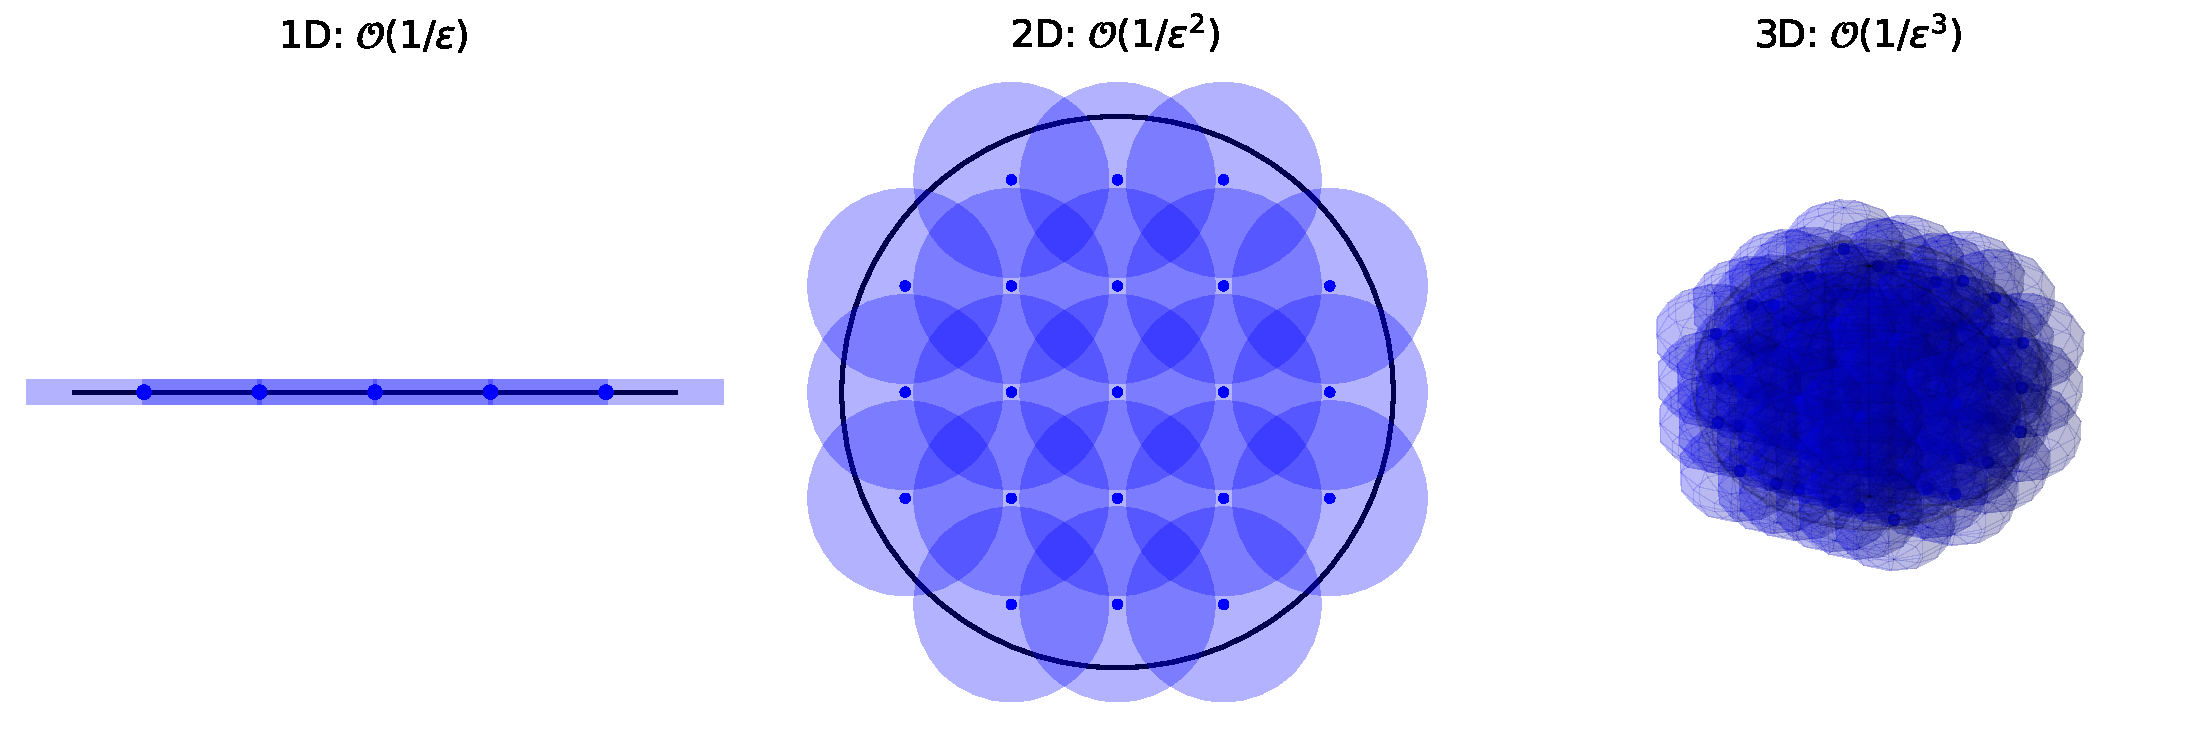
\includegraphics[width=0.95\textwidth]{epsilon_net.pdf}
\caption{Representación visual del crecimiento exponencial del número de recubrimiento $\mathcal{N}(\mathbb{S}^{d-1}, \epsilon)$. A medida que aumenta la dimensión $d$, la cantidad de muestras (centros en azul) de radio $\epsilon$ requeridas para cubrir el volumen completo sin dejar agujeros crece exponencialmente como $\mathcal{O}((1/\epsilon)^d)$.}
\label{fig:epsilon_net_dimension}
\end{figure}

\chapter{La Revolución No Contrastiva: Decorrelación y el Principio de Barlow}
\label{cap:nocontrastive}

La búsqueda de métodos independientes de las muestras negativas condujo a una de las intersecciones más ricas entre la neurobiología teórica y el aprendizaje de representaciones: la aplicación del principio de Barlow. Este capítulo detalla los fundamentos matemáticos de las pérdidas basadas en la correlación cruzada (Barlow Twins) y la regularización explícita de covarianza (VICReg).

\section{La Hipótesis de Reducción de Redundancia de Barlow (1961)}
\label{sec:barlow_hipotesis}
En 1961, el neurobiólogo Horace Barlow formuló la \textbf{hipótesis de codificación eficiente}, planteando que nuestro sistema nervioso no procesa los estímulos sensoriales en bruto, sino que los recodifica de modo que la actividad de las neuronas individuales sea, en la medida de lo posible, estadísticamente \textit{independiente} \cite{barlow1961possible}. La idea se apoyaba en trabajos previos de Shannon, quien había mostrado que sistemas naturales como el lenguaje contienen una redundancia considerable. En ellos, gran parte de la señal es predecible a partir del resto, y por tanto no aporta información nueva en el sentido de Shannon. Una codificación óptima, bajo esta perspectiva, es aquella que elimina dicha redundancia y representa la señal con el menor número de símbolos estadísticamente correlacionados entre sí.

Al trasladar este principio a la biología, Barlow observó que nuestro entorno presenta fuertes correlaciones espaciotemporales. Por ejemplo, la luminancia en regiones contiguas del campo visual rara vez varía de forma abrupta, de manera que transmitir cada píxel o cada instante de forma independiente supondría malgastar buena parte de la capacidad del canal neuronal en información redundante, con un coste metabólico que el cerebro no puede permitirse. Para resolverlo, la corteza sensorial actuaría como un filtro que suprime esa redundancia, proyectando las señales de entrada sobre un nuevo espacio de características mutuamente independientes. La red, así, no necesita gastar recursos en lo que ya es predecible a partir del contexto inmediato, y puede reservarlos para aquello que realmente constituye información nueva.

\subsection{La Información Mutua como Medida Ideal de Independencia}

Para formalizar la hipótesis de reducción de redundancia de Barlow, el objetivo es asegurar que las componentes del vector de \textit{embeddings} $Z = (z_1, z_2, \dots, z_d)$ extraído por un modelo sean lo más independientes posible.

En estadística elemental, la independencia suele aproximarse mediante la \textbf{correlación lineal} de Pearson ($\rho$). Sin embargo, como principal limitación, ésta solo detecta relaciones lineales. Para medir la dependencia de forma exhaustiva y fiel, la métrica ideal es la \textbf{Información Mutua} ($I$) de la teoría de la información de Shannon \cite{shannon1948mathematical}. A diferencia de la correlación, la información mutua captura \textit{cualquier} tipo de dependencia (lineal o no lineal) y es invariante ante transformaciones complejas, garantizando una medición más precisa de la redundancia.

De acuerdo con Shannon, la información individual de una característica $z_i$ queda definida por su \textbf{entropía} $H(z_i) = \mathbb{E}[-\log p(z_i)]$. Análogamente, la \textbf{entropía conjunta} $H(z_i, z_j)$ mide la información total del par, donde $p(z_i)$ y $p(z_i,z_j)$ denotan las distribuciones poblacionales marginal y conjunta, respectivamente. Hay que señalar que estas formulaciones asumen el conocimiento de la ley de probabilidad subyacente sobre la que se distribuyen los datos, la cual es estrictamente inobservable y en consecuencia, requiere ser inferida a partir de una muestra finita de datos.

La información mutua se define entonces como la información compartida por dos variables o símbolos de la representación:
\begin{equation}
I(z_i; z_j) = H(z_i) + H(z_j) - H(z_i, z_j)
\end{equation}
Si $z_i$ y $z_j$ son totalmente independientes, su información mutua es cero: $I(z_i; z_j) = 0$, y su entropía conjunta es la suma de las partes: $H(z_i, z_j) = H(z_i) + H(z_j)$. Esta idea puede extenderse a todo el vector de características. Para ello construimos la \textbf{matriz de información mutua} $\mathcal{I}(Z) \in \mathbb{R}^{d \times d}$:
\begin{equation}
\mathcal{I}(Z)_{ij} = 
\begin{cases}
H(z_i) & \text{si } i = j \\
I(z_i; z_j) & \text{si } i \neq j
\end{cases}
\end{equation}

El \textbf{ideal de Barlow} equivale, teóricamente, a conseguir que $\mathcal{I}(Z)$ sea una \textbf{matriz diagonal}. Esto significa que no hay información compartida entre características distintas: $I(z_i; z_j) = 0$, mientras que cada neurona individual (recordemos que en nuestra arquitectura cada componente $z_i$ representa la activación de una neurona en la capa de proyección de salida) retiene la máxima información posible $H(z_i)$, evitando así el colapso de las representaciones.

\begin{figure}[h!]
    \centering
    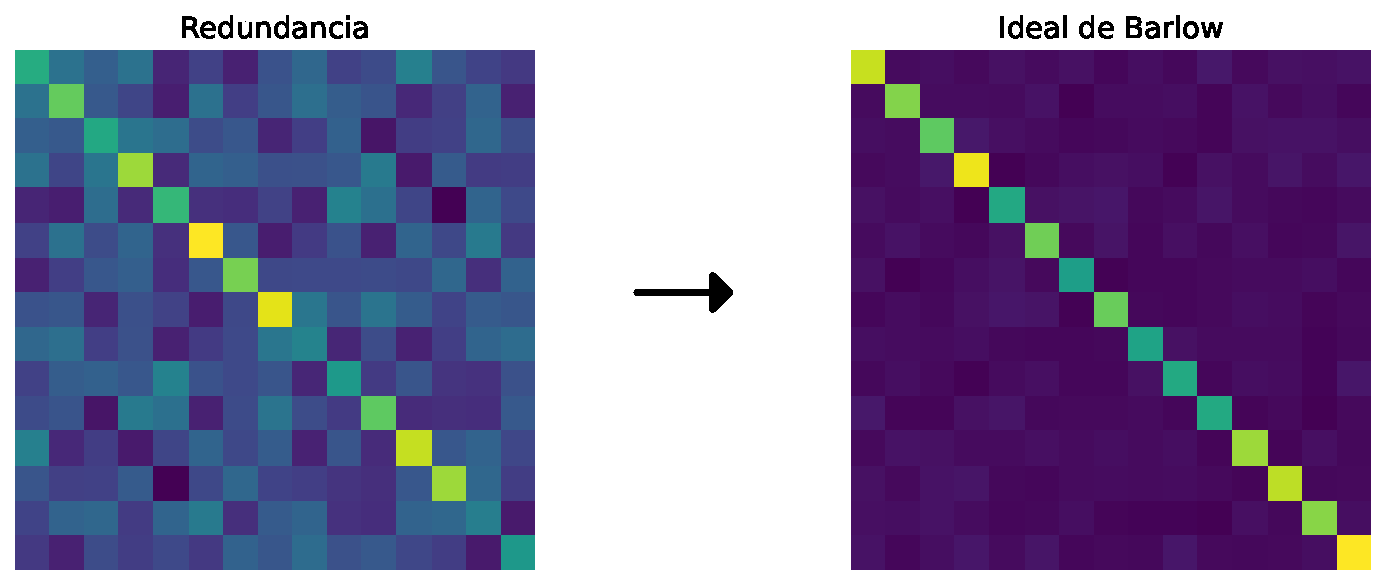
\includegraphics[width=0.9\textwidth]{heatmaps_IZ.pdf}
    \caption{Visualización conceptual de la matriz de información mutua $\mathcal{I}(Z)$ (simétrica), donde los ejes representan las neuronas de la capa de salida, o equivalentemente, las dimensiones de la codificación. La primera matriz corresponde a una representación redundante, donde existen dependencias significativas entre distintas componentes (valores no despreciables fuera de la diagonal). En el \textit{Ideal de Barlow}, la matriz presenta una estructura casi diagonal, donde las componentes son mutuamente independientes y cada una retiene su entropía individual máxima.}
    \label{fig:heatmaps_IZ}
\end{figure}

\subsection{El Puente de Jaynes}

Estimar la información mutua y la entropía de Shannon es computacionalmente intratable en espacios no triviales donde se desconoce la distribución subyacente de los datos. Sin embargo, cuando los datos se distribuyen de forma gaussiana, la expresión de la información mutua se reduce a una expresión que depende exclusivamente del coeficiente de correlación lineal de Pearson ($\rho_{ij}$).

\begin{proposition}[Puente de Jaynes]
Sea $(z_i, z_j)$ un par de representaciones distribuidas conjuntamente según una distribución normal con coeficiente de correlación de Pearson $\rho_{ij}$. Entonces, la información mutua de Shannon entre ambas variables viene dada por:
\begin{equation}
I(z_i; z_j) = -\frac{1}{2} \log(1 - \rho_{ij}^2)
\end{equation}
\end{proposition}

\begin{proof}
Sea $(z_i, z_j)$ siguiendo una distribución normal bivariante:
\begin{equation}
\begin{pmatrix} z_i \\ z_j \end{pmatrix} \sim \mathcal{N}\left( \begin{pmatrix} \mu_i \\ \mu_j \end{pmatrix}, \Sigma \right)
\end{equation}
Recordemos la funcion de densidad normal multivariante en el caso general:
\begin{equation}
p(Z) = \frac{1}{\sqrt{(2\pi)^k det(\Sigma)}} e^{ -\frac{1}{2}(Z-\mu)^\top \Sigma^{-1} (Z-\mu) }
\end{equation}

Aplicando la definición de entropía de Shannon y las propiedades del logaritmo:
\begin{equation}
\begin{aligned}
H(Z) &= \mathbb{E}[-\log p(Z)] \\
     &= \mathbb{E}\left[ \frac{1}{2} \log((2\pi)^k det(\Sigma)) + \frac{1}{2}(Z-\mu)^\top \Sigma^{-1} (Z-\mu) \right] \\
     &= \frac{1}{2} \log((2\pi)^k det(\Sigma)) + \frac{1}{2}\mathbb{E}\left[(Z-\mu)^\top \Sigma^{-1} (Z-\mu) \right]
\end{aligned}
\end{equation}

Aplicando $A \in \mathbb{R} \implies Tr(A) = A $ , $Tr(AB) = Tr(BA)$, $\Sigma = \mathbb{E}[(Z-\mu)(Z-\mu)^\top$:

\begin{equation}
\begin{aligned}
 \mathbb{E}\left[(Z-\mu)^\top \Sigma^{-1} (Z-\mu) \right] &= \mathbb{E}[\text{tr}((Z-\mu)^\top\Sigma^{-1} (Z-\mu))] \\ &= \text{tr}(\Sigma^{-1} \mathbb{E}[(Z-\mu)(Z-\mu)^\top]) \\ 
 &= \text{tr}(\Sigma^{-1} \Sigma) = \text{tr}(I_k) \\ 
 &= k
\end{aligned}
\end{equation}

Sustituyendo, agrupando y usando las propiedades de los logaritmos:
\begin{equation}
\begin{aligned}
H(Z) &= \frac{1}{2} \log((2\pi)^2 det(\Sigma)) + \frac{k}{2} \\ 
     &= \frac{1}{2} \log((2\pi)^2 det(\Sigma)) + \frac{1}{2}\log(e^k) \\
     &= \frac{1}{2} \log \left( (2\pi e)^k det(\Sigma) \right)
\end{aligned}
\end{equation}

Para evaluar la entropía conjunta $H(z_i, z_j)$, aplicamos la fórmula anterior particularizada para el caso $k=2$. Usando la relación $\Sigma_{ij} = \rho_{ij}\sqrt{\Sigma_{ii}\Sigma_{jj}}$, calculamos el determinante de la matriz de covarianza:

\begin{equation}
\begin{aligned} 
det(\Sigma) &= \Sigma_{ii}\Sigma_{jj} - \Sigma_{ij}^2 \\
            &= \Sigma_{ii}\Sigma_{jj} - \left( \rho_{ij}\sqrt{\Sigma_{ii}\Sigma_{jj}} \right)^2 \\
            &= \Sigma_{ii}\Sigma_{jj} - \rho_{ij}^2 \Sigma_{ii}\Sigma_{jj} \\ 
            &= \Sigma_{ii}\Sigma_{jj}(1 - \rho_{ij}^2)
\end{aligned}
\end{equation}

Por tanto la expresión de la entropía queda:
\begin{equation}
H(z_i, z_j) = \frac{1}{2} \log \left( (2\pi e)^2 \Sigma_{ii}\Sigma_{jj} (1 - \rho_{ij}^2) \right)
\end{equation}

Por su parte, las distribuciones marginales $p(z_i)$ y $p(z_j)$ resultan ser también gaussianas, pero en este caso unidimensionales ($k=1$), con varianzas $\Sigma_{ii}$ y $\Sigma_{jj}$ respectivamente. Por tanto, sus entropías marginales individuales son:
\begin{equation}
H(z_i) = \frac{1}{2} \log(2\pi e \Sigma_{ii}), \quad H(z_j) = \frac{1}{2} \log(2\pi e \Sigma_{jj})
\end{equation}

Aplicando la definición de información mutua y usando las propiedades algebraicas del logaritmo:
\begin{equation}
\begin{aligned}
I(z_i; z_j) &= H(z_i) + H(z_j) - H(z_i, z_j) \\
            &= \frac{1}{2} \log(2\pi e \Sigma_{ii}) + \frac{1}{2} \log(2\pi e \Sigma_{jj}) - \frac{1}{2} \log \left( (2\pi e)^2 \Sigma_{ii}\Sigma_{jj} (1 - \rho_{ij}^2) \right) \\
            &= \frac{1}{2} \log \left( \frac{(2\pi e \Sigma_{ii})(2\pi e \Sigma_{jj})}{(2\pi e)^2 \Sigma_{ii}\Sigma_{jj} (1 - \rho_{ij}^2)} \right) \\
            &= \frac{1}{2} \log \left( \frac{(2\pi e)^2 \Sigma_{ii}\Sigma_{jj}}{(2\pi e)^2 \Sigma_{ii}\Sigma_{jj} (1 - \rho_{ij}^2)} \right) \\
            &= -\frac{1}{2} \log(1 - \rho_{ij}^2)
\end{aligned}
\end{equation}
\end{proof}

En consecuencia, bajo el supuesto de que las representaciones siguen una distribución gaussiana, la correlación lineal basta para capturar la totalidad de las dependencias estadísticas. En este caso forzar la decorrelación lineal es suficiente para garantizar la independencia. El siguiente corolario muestra cómo esto nos permite simplificar la optimización de la matriz de información mutua $\mathcal{I}(Z)$:

\begin{corollary}[Equivalencia Matricial]
Sea $Z \in \mathbb{R}^d$ un vector de representaciones que sigue una distribución normal multivariante, $\mathcal{I}(Z) \in \mathbb{R}^{d \times d}$ su matriz de información mutua y $R \in \mathbb{R}^{d \times d}$ su matriz de correlación lineal. Bajo la hipótesis de normalidad, garantizar la independencia es equivalente a imponer la decorrelación lineal:
\begin{equation}
\mathcal{I}(Z) \text{ es diagonal } \iff R = I_d
\end{equation}
donde $I_d$ denota la matriz identidad de dimensión $d$.
\end{corollary}

\begin{proof}
Por definición, los elementos de la diagonal principal de cualquier matriz de correlación $R$ son iguales a la unidad ($R_{ii} = \rho_{ii} = 1$). Para los elementos fuera de la diagonal ($i \neq j$), la proposición del Puente de Jaynes establece que:
\begin{equation}
I(z_i; z_j) = -\frac{1}{2} \log(1 - \rho_{ij}^2)
\end{equation}

La matriz $\mathcal{I}(Z)$ es diagonal si y solo si la información mutua entre características distintas es nula, es decir, $I(z_i; z_j) = 0$ para todo $i \neq j$. Igualando a cero la expresión matricial obtenemos:
\begin{equation}
-\frac{1}{2} \log(1 - \rho_{ij}^2) = 0 \iff \log(1 - \rho_{ij}^2) = 0 \iff 1 - \rho_{ij}^2 = 1 \iff \rho_{ij} = 0
\end{equation}

Por consiguiente, exigir que $I(z_i; z_j) = 0$ para todo $i \neq j$ equivale a imponer que $\rho_{ij} = 0$ para todo $i \neq j$. Dado que los elementos diagonales de $R$ son iguales a $1$, esta condición equivale a $R = I_d$.
\end{proof}

\section{La Arquitectura Barlow Twins}
\label{sec:barlow_twins}

Propuesto por Zbontar et al. en 2021 \cite{zbontar2021barlow}, el método Barlow Twins traduce el principio de reducción de redundancia de Barlow de la sección anterior a un marco práctico de aprendizaje auto-supervisado.

\begin{figure}[H]
    \centering
    \begin{tikzpicture}[
        node distance=1.5cm and 2cm,
        box/.style={draw, rectangle, rounded corners, minimum width=2.2cm, minimum height=1.2cm, align=center, fill=blue!5},
        img/.style={draw, rectangle, rounded corners, minimum width=1.5cm, minimum height=1.5cm, fill=orange!10, align=center},
        mat/.style={draw, rectangle, minimum width=2.5cm, minimum height=2.5cm, fill=green!5, align=center},
        arrow/.style={->, >=stealth, thick}
    ]
        \node (x) {Observación $x$};
        \node[img, above right=0.5cm and 0.8cm of x] (ya) {Vista $A$\\$x_1 = t^A(x)$};
        \node[img, below right=0.5cm and 0.8cm of x] (yb) {Vista $B$\\$x_2 = t^B(x)$};
        \node[box, right=0.8cm of ya] (enc_a) {Red\\$f_\theta$};
        \node[box, right=0.8cm of yb] (enc_b) {Red\\$f_\theta$};
        \node[right=0.6cm of enc_a] (za) {$z^A$};
        \node[right=0.6cm of enc_b] (zb) {$z^B$};
        \node[mat, right=1.2cm of za, yshift=-1.6cm] (matrix) {Correlación\\Cruzada $C$};
        \node[right=0.8cm of matrix, font=\Large] (identidad) {$I_d$};
        
        \draw[arrow] (x.east) to[out=0, in=180] (ya.west);
        \draw[arrow] (x.east) to[out=0, in=180] (yb.west);
        \draw[arrow] (ya) -- (enc_a);
        \draw[arrow] (yb) -- (enc_b);
        \draw[arrow] (enc_a) -- (za);
        \draw[arrow] (enc_b) -- (zb);
        \draw[arrow] (za.east) to[out=0, in=180] (matrix.150);
        \draw[arrow] (zb.east) to[out=0, in=180] (matrix.210);
        \draw[<->, >=stealth, thick, red] (matrix.east) -- node[above, text=black] {$\mathcal{L}_{\mathcal{BT}}$} (identidad.west);
        \draw[<->, dashed, thick, gray] (enc_a.south) -- node[right, text=black, align=center, text width=2.5cm] {Pesos compartidos} (enc_b.north);
    \end{tikzpicture}
    \caption{Esquema de arquitectura Barlow Twins. Dos transformaciones aleatorias $t^A$ y $t^B$ generan vistas distorsionadas de $x$. Ambas se procesan con redes siamesas $f_\theta$ para obtener $z^A$ y $z^B$. Se calcula la matriz de correlación cruzada $C$ sobre el minibatch y se minimiza su discrepancia respecto a $I_d$.}
    \label{fig:barlow_twins_arch}
\end{figure}

\subsection{Construcción de las Vistas y Representaciones}

Dada una observación $x$, se generan dos vistas $x_1$ y $x_2$ mediante transformaciones aleatorias independientes $t^A, t^B$ (p.e. recortes, \textit{masking}, variaciones de color). Ambas vistas $x_1 = t^A(x)$ y $x_2 = t^B(x)$ se procesan con la misma red $f_\theta$ (pesos compartidos), produciendo dos representaciones vectoriales en $\mathbb{R}^d$:
\begin{equation}
z^A = f_\theta(x_1), \qquad z^B = f_\theta(x_2).
\end{equation}
En un escenario ideal donde el modelo fuese totalmente invariante a las transformaciones aplicadas, se cumpliría $z^A = z^B$. Sobre un minibatch de $N$ pares compatibles $\{(x_1^{(i)}, x_2^{(i)})\}_{i=1}^N$, apilamos las representaciones de cada vista en una matriz de batch:
\begin{equation}
Z^A, Z^B \in \mathbb{R}^{N \times d}, \qquad \text{donde la fila } i \text{ de } Z^A \text{ es } z^{A,(i)} = f_\theta(x_1^{(i)}) \in \mathbb{R}^d,
\end{equation}
y análogamente para $Z^B$ con $z^{B,(i)} = f_\theta(x_2^{(i)})$. Cada fila es una observación del minibatch; cada columna representa una dimensión del espacio latente. Denotaremos por $z_k^{A,(i)}$ la entrada $(i,k)$ de $Z^A$, es decir, el valor de la dimensión $k$ de la representación de la vista $A$ para la observación $i$.

\subsection{El Centrado en Media}

Antes de poder hablar de correlación, las representaciones deben estar \textbf{centradas en media}: para cada vista y cada dimensión $k$, se resta su media empírica sobre el minibatch,
\begin{equation}
z_k^{A,(i)} \gets z_k^{A,(i)} - \frac{1}{N}\sum_{m=1}^N z_k^{A,(m)}, \qquad z_k^{B,(i)} \gets z_k^{B,(i)} - \frac{1}{N}\sum_{m=1}^N z_k^{B,(m)},
\end{equation}
Esto centra cada columna de $Z^A$ y de $Z^B$ a media cero. La razón de exigir esto es simple: si las representaciones no estuvieran centradas, el producto escalar entre columnas estaría dominado por un término de medias de magnitud elevada, enmascarando la verdadera covarianza entre dimensiones. El centrado garantiza que lo que optimicemos a continuación sean auténticas correlaciones, y no simples momentos de segundo orden no centrados.

\subsection{La Matriz de Correlación Cruzada}

Con $Z^A, Z^B \in \mathbb{R}^{N \times d}$ (ya centradas por columnas), denotemos por $\mathbf{z}_k^A, \mathbf{z}_l^B \in \mathbb{R}^N$ la columna $k$-ésima de $Z^A$ y la columna $l$-ésima de $Z^B$, respectivamente, es decir, $\mathbf{z}_k^A = (z_k^{A,(1)}, \dots, z_k^{A,(N)})^\top$.

\begin{definition}[Matriz de Correlación Cruzada Empírica]
La matriz de correlación cruzada $C \in \mathbb{R}^{d \times d}$ se define entrada a entrada como la similitud coseno entre las columnas $k$-ésima de $Z^A$ y $l$-ésima de $Z^B$:
\begin{equation}
C_{kl} = \frac{\langle \mathbf{z}_k^A, \mathbf{z}_l^B \rangle}{\|\mathbf{z}_k^A\|_2 \, \|\mathbf{z}_l^B\|_2} = \frac{\sum_{i=1}^{N} z_k^{A,(i)} z_l^{B,(i)}}{\sqrt{\sum_{i=1}^{N} (z_k^{A,(i)})^2} \sqrt{\sum_{i=1}^{N} (z_l^{B,(i)})^2}}, \qquad C_{kl} \in [-1,1].
\end{equation}
Equivalentemente, en notación matricial: $C = (Z^A)^\top Z^B$ tras normalizar cada columna de $Z^A$ y $Z^B$ a norma unidad.
\end{definition}

\begin{figure}[H]
    \centering
    % El uso de \resizebox asegura que la figura nunca exceda el ancho de la página.
    % Requiere tener \usepackage{graphicx} en el preámbulo.
    \resizebox{\linewidth}{!}{
    \begin{tikzpicture}[
        every node/.style={font=\footnotesize},
        mathnode/.style={font=\footnotesize, minimum width=0.6cm, minimum height=0.45cm},
        highlight/.style={fill=orange!15, draw=orange!70!black, thick},
        highlightB/.style={fill=blue!10, draw=blue!60!black, thick},
        cellhighlight/.style={fill=green!15, draw=green!50!black, thick}
    ]

    % ============================================================
    % MATRIZ Z^A
    % ============================================================
    \matrix (ZA) [
        matrix of math nodes,
        nodes={mathnode},
        ampersand replacement=\&,
        left delimiter={(}, right delimiter={)},
        column sep=1pt, row sep=1pt,
        anchor=center
    ]
    {
        z_1^{A,(1)} \& \cdots \& z_k^{A,(1)} \& \cdots \& z_d^{A,(1)} \\
        z_1^{A,(2)} \& \cdots \& z_k^{A,(2)} \& \cdots \& z_d^{A,(2)} \\
        \vdots      \&        \& \vdots      \&        \& \vdots      \\
        z_1^{A,(N)} \& \cdots \& z_k^{A,(N)} \& \cdots \& z_d^{A,(N)} \\
    };
    \begin{scope}[on background layer]
        \node[highlight, fit=(ZA-1-3)(ZA-4-3), inner sep=1pt] (colA) {};
    \end{scope}
    \node[above=0.1cm of ZA] {$Z^A \in \mathbb{R}^{N \times d}$};
    \node[below=0.1cm of colA, text=orange!70!black] {dimensión $k$: $\mathbf{z}_k^A$};
    \node[font=\footnotesize, text=gray!80!black, rotate=90] at ([xshift=-0.6cm]ZA.west) {$\longleftarrow$ observaciones $\longrightarrow$};

    % ============================================================
    % MATRIZ Z^B
    % ============================================================
    \matrix (ZB) [
        matrix of math nodes,
        nodes={mathnode},
        ampersand replacement=\&,
        left delimiter={(}, right delimiter={)},
        column sep=1pt, row sep=1pt,
        anchor=center,
        right=0.6cm of ZA
    ]
    {
        z_1^{B,(1)} \& \cdots \& z_l^{B,(1)} \& \cdots \& z_d^{B,(1)} \\
        z_1^{B,(2)} \& \cdots \& z_l^{B,(2)} \& \cdots \& z_d^{B,(2)} \\
        \vdots      \&        \& \vdots      \&        \& \vdots      \\
        z_1^{B,(N)} \& \cdots \& z_l^{B,(N)} \& \cdots \& z_d^{B,(N)} \\
    };
    \begin{scope}[on background layer]
        \node[highlightB, fit=(ZB-1-3)(ZB-4-3), inner sep=1pt] (colB) {};
    \end{scope}
    \node[above=0.1cm of ZB] {$Z^B \in \mathbb{R}^{N \times d}$};
    \node[below=0.1cm of colB, text=blue!60!black] {dimensión $l$: $\mathbf{z}_l^B$};

    % ============================================================
    % MATRIZ C
    % ============================================================
    \matrix (C) [
        matrix of math nodes,
        nodes={mathnode},
        ampersand replacement=\&,
        left delimiter={(}, right delimiter={)},
        column sep=1pt, row sep=1pt,
        anchor=center,
        right=0.6cm of ZB
    ]
    {
        C_{11} \& \cdots \& C_{1l} \& \cdots \& C_{1d} \\
        \vdots \&        \& \vdots \&        \& \vdots \\
        C_{k1} \& \cdots \& C_{kl} \& \cdots \& C_{kd} \\
        \vdots \&        \& \vdots \&        \& \vdots \\
        C_{d1} \& \cdots \& C_{dl} \& \cdots \& C_{dd} \\
    };
    \begin{scope}[on background layer]
        \node[cellhighlight, fit=(C-3-3), inner sep=1pt] (cellKL) {};
    \end{scope}
    \node[above=0.1cm of C] {$C \in \mathbb{R}^{d \times d}$};

    % ============================================================
    % FÓRMULA CENTRAL
    % ============================================================
    \node[
        below=0.6cm of C,
        anchor=center
    ] (dotprod) {
        \textcolor{green!50!black}{$C_{kl}$} $= \dfrac{\langle {\mathbf{z}_k^A}, {\mathbf{z}_l^B} \rangle}
        {\|{\mathbf{z}_k^A}\|_2 \, \|{\mathbf{z}_l^B}\|_2}$
    };

    \end{tikzpicture}
    }
    \caption{Construcción de la matriz de correlación cruzada $C$ mediante el producto escalar normalizado (similitud coseno) entre las columnas de $Z^A$ y $Z^B$.}
    \label{fig:cross_corr_matrices_horizontal_compact}
\end{figure}

\begin{definition}[Función de Pérdida de Barlow Twins]
La pérdida penaliza la discrepancia de $C$ respecto a la identidad $I_d$:
\begin{equation}
\mathcal{L}_{\mathcal{BT}} = \underbrace{\sum_{k=1}^{d} (1 - C_{kk})^2}_{\text{Invarianza}} + \lambda \underbrace{\sum_{k=1}^{d} \sum_{l \neq k} C_{kl}^2}_{\text{Redundancia}},
\end{equation}
\end{definition} 
\noindent siendo $\lambda > 0$ un hiperparámetro que pondera los dos objetivos de la pérdida. Análogamente a cómo el margen en las pérdidas contrastivas regula la repulsión entre muestras negativas, aquí $\lambda$ modula la repulsión \textit{entre características}. Cada término de $\mathcal{L}_{\mathcal{BT}}$ tiene una interpretación geométrica derivada de la construcción de $C$:

\begin{itemize}
    \item \textbf{Invarianza ($C_{kk} \to 1$):} $C_{kk}$ es la similitud coseno entre la columna $k$ de $Z^A$ y la columna $k$ de $Z^B$, es decir, entre los valores que la dimensión $k$ asume en la vista $A$ y en la vista $B$ a lo largo de todo el minilote. Forzar $C_{kk} \to 1$ exige que ambas columnas sean proporcionales en $\mathbb{R}^N$; por la desigualdad de Cauchy-Schwarz, esto ocurre si y solo si $\mathbf{z}_k^A = c \cdot \mathbf{z}_k^B$ con $c > 0$, es decir, que la red extraiga la misma información en la dimensión $k$ con independencia de la vista procesada.

    \item \textbf{Reducción de redundancia ($C_{kl} \to 0$, $k \neq l$):} durante el entrenamiento las vistas difieren ($Z^A \neq Z^B$), por lo que $C_{kl}$ captura la correlación cruzada entre la dimensión $k$ de la vista $A$ y la dimensión $l$ de la vista $B$. Forzar $C_{kl} \to 0$ equivale a imponer $\langle \mathbf{z}_k^A, \mathbf{z}_l^B \rangle \to 0$, es decir, ortogonalidad cruzada entre dimensiones distintas de las dos vistas. Cada dimensión queda así obligada a codificar información que las demás no capturan, repartiendo la varianza semántica por todo $\mathbb{R}^d$ de acuerdo con el principio de Barlow.
\end{itemize}

La matriz empírica $C$ aproxima, en cada minibatch, la correlación cruzada poblacional $\mathcal{C}_{kl} = \mathbb{E}[Z_k^A Z_l^B] / \sqrt{\mathbb{E}[(Z_k^A)^2]\mathbb{E}[(Z_l^B)^2]}$ definida sobre la distribución de pares positivos $p_{\text{pos}}(x_1,x_2)$. Barlow Twins emplea la correlación \textit{cruzada} en lugar de la autocorrelación precisamente porque, durante el entrenamiento, $Z^A \neq Z^B$: al operar con $C$, el método mide y minimiza simultáneamente la discrepancia entre vistas en la diagonal y la redundancia entre características fuera de ella.

La conexión con la teoría de Barlow se vuelve exacta en el \textbf{límite de invarianza perfecta}. Cuando el modelo asimila ambas vistas idénticamente ($Z^A = Z^B = Z$), cada par de columnas colapsa a un único vector ($\mathbf{z}_k^A = \mathbf{z}_k^B = \mathbf{z}_k$), y la correlación cruzada $\mathcal{C}$ se reduce a la matriz de autocorrelación de Pearson $R$ de la Sección~\ref{sec:barlow_hipotesis}. En ese límite, forzar $\mathcal{C} \to I_d$ equivale estrictamente a imponer $R \to I_d$, logrando la decorrelación que exige el principio original.


En resumen, Barlow Twins evita el colapso de las \textit{Joint Embedding Architectures} sin recurrir a muestras negativas ni a mecanismos arquitectónicos auxiliares. Basta con imponer $C \to I_d$, condición que, como establece el Puente de Jaynes (Sección~\ref{sec:barlow_hipotesis}), es matemáticamente equivalente a exigir la independencia estadística entre las dimensiones del espacio $\mathcal{Z}$.

\section{VICReg: Desacoplamiento de Varianza, Invarianza y Covarianza}
\label{sec:vicreg}

La elección de la matriz de correlación cruzada $C$ como objeto central de la optimización en Barlow Twins conlleva algunos problemas de diseño. Recordemos que cada entrada $C_{kl}$ se obtiene dividiendo el producto escalar entre las columnas $\mathbf{z}_k^A$ y $\mathbf{z}_l^B$ por el producto de sus normas euclídeas. Esto hace que el objeto de optimización ignore la escala de las representaciones, centrándose únicamente en las direcciones.

\begin{proposition}[Invarianza de $C$ ante reescalado]
\label{prop:C_escala}
Sea $C$ la matriz de correlación cruzada definida en la Sección~\ref{sec:barlow_twins}. Para cualquier reescalado positivo por dimensiones $z_j \mapsto \alpha_j z_j$ con $\alpha_j > 0$, la matriz $C$ permanece inalterada.
\end{proposition}

\begin{proof}
Sea $\tilde{\mathbf{z}}_k^A = \alpha_k \mathbf{z}_k^A$ la columna $k$-ésima de $Z^A$ tras el reescalado. Entonces:
\begin{equation}
\tilde{C}_{kl} = \frac{\langle \tilde{\mathbf{z}}_k^A, \tilde{\mathbf{z}}_l^B \rangle}{\|\tilde{\mathbf{z}}_k^A\|_2 \, \|\tilde{\mathbf{z}}_l^B\|_2} = \frac{\alpha_k \alpha_l \langle \mathbf{z}_k^A, \mathbf{z}_l^B \rangle}{\alpha_k \|\mathbf{z}_k^A\|_2 \cdot \alpha_l \|\mathbf{z}_l^B\|_2} = \frac{\langle \mathbf{z}_k^A, \mathbf{z}_l^B \rangle}{\|\mathbf{z}_k^A\|_2 \, \|\mathbf{z}_l^B\|_2} = C_{kl}.
\end{equation}
Los factores $\alpha_k$ y $\alpha_l$ se cancelan exactamente por la normalización.
\end{proof}

Por tanto, la formulación Barlow Twins basada en la matriz de correlación cruzada $C$ presenta dos problemas fundamentales que limitan su capacidad de regularización:

\begin{enumerate}
    \item Colapso dimensional por ausencia de sensibilidad a la escala.
    \item Acoplamiento de objetivos (\textit{entanglement}).
\end{enumerate}

Respecto al primer problema, la Proposición~\ref{prop:C_escala} implica que $C$ descarta toda información sobre la \emph{escala} de las dimensiones de $\mathcal{Z}$. En particular, reducir la varianza de una dimensión $j$ a un valor arbitrariamente pequeño no modifica los elementos diagonales $C_{jj}$ ya que están normalizados. Recordemos que si una dimensión tiene varianza nula, significa que la red está emitiendo exactamente el mismo valor numérico para todas las imágenes a lo largo de esa coordenada; esta es precisamente la manifestación empírica del colapso dimensional. Esto plantea un grave problema, una dimensión colapsada (cuya varianza tiende a cero por no codificar información útil) puede mantener un valor óptimo $C_{jj} \approx 1$ siempre que las fluctuaciones residuales en $\mathbf{z}_j^A$ y $\mathbf{z}_j^B$ estén alineadas. La pérdida $\mathcal{L}_{\mathcal{BT}}$ no distingue entre una dimensión con varianza unitaria y otra con varianza despreciable, ambas contribuyen de forma idéntica a la diagonal de $C$. Por tanto, $\mathcal{L}_{\mathcal{BT}}$ carece de un mecanismo explícito para garantizar que todas las dimensiones del espacio $\mathcal{Z}$ mantengan una dispersión suficiente.

El segundo problema surge de condensar los objetivos de invarianza ($C_{kk} \to 1$) y de decorrelación ($C_{kl} \to 0$) en un único objeto, la matriz $C$. Como ambos términos comparten el mismo denominador de normalización, no pueden tratarse de forma independiente: cualquier perturbación se propaga simultáneamente a la diagonal y a la parte fuera de la diagonal de $C$, acoplando así dos objetivos que, en principio, son conceptualmente distintos, Bardes et al.~\cite{bardes2022vicreg}.

Resulta natural preguntarse si es posible evitar estas limitaciones formulando una función de pérdida que \emph{desacople} explícitamente la invarianza, la dispersión dimensional y la independencia entre características, sobre un objeto que retenga la información de escala que $C$ descarta. VICReg (\textit{Variance-Invariance-Covariance Regularization}), propuesto por Bardes, Ponce y LeCun en 2022~\cite{bardes2022vicreg}, ofrece dicha formulación.

\subsection{De la correlación cruzada a la covarianza}

\begin{definition}[Matriz de Covarianza Empírica]
\label{def:cov_empirica_vicreg}
Sea $Z \in \mathbb{R}^{N \times d}$ una matriz de embeddings correspondiente a un batch de $N$ observaciones, y sea $\bar{z} = \frac{1}{N}\sum_{i=1}^{N} z^{(i)} \in \mathbb{R}^d$ su vector de medias. La matriz de covarianza empírica se define como:
\begin{equation}
\label{eq:cov_empirica_vicreg}
\Sigma_\mathcal{Z} = \frac{1}{N-1} \sum_{i=1}^{N} (z^{(i)} - \bar{z})(z^{(i)} - \bar{z})^\top = \frac{1}{N-1} (Z - \bar{Z})^\top (Z - \bar{Z}) \in \mathbb{R}^{d \times d},
\end{equation}
donde $\bar{Z} \in \mathbb{R}^{N \times d}$ denota la matriz cuyas $N$ filas son todas iguales a $\bar{z}^\top$. El elemento $(\Sigma_\mathcal{Z})_{kl}=\operatorname{Cov}(z_{k},z_{l})$ es la covarianza empírica entre las dimensiones $k$ y $l$ a lo largo del batch, y en particular $(\Sigma_\mathcal{Z})_{jj} = \operatorname{Var}(z_{j})$ es la varianza empírica de la dimensión $j$.
\end{definition}

La idea central de VICReg consiste en usar esta matriz de covarianza empírica en lugar de la matriz de correlación cruzada $C$ de la Sección~\ref{sec:barlow_twins}. Nótese que este objeto ya fue introducido en un contexto poblacional en la Sección~\ref{sec:colapso_dimensional_v2}; aquí empleamos su versión empírica, o estimador sobre el batch. A diferencia de $C$, cuyos elementos satisfacen $C_{kl} \in [-1,1]$ por construcción, los elementos de $\Sigma_\mathcal{Z}$ no están acotados ni normalizados. Para comprender qué información pierde $C$ respecto a $\Sigma_\mathcal{Z}$, veremos la relación entre ambos objetos.

En el límite analizado al final de la Sección~\ref{sec:barlow_twins} ($Z^A = Z^B = Z$), la correlación cruzada $C$ se reduce a la matriz de autocorrelación $R$ de una única vista. La relación entre $R$ y la covarianza $\Sigma_\mathcal{Z}$ de un mismo vector aleatorio es la siguiente: 
\begin{equation}
\label{eq:relacion_R_Sigma}
R_{kl} = \frac{(\Sigma_\mathcal{Z})_{kl}}{\sqrt{(\Sigma_\mathcal{Z})_{kk}}\,\sqrt{(\Sigma_\mathcal{Z})_{ll}}}.
\end{equation}

La ecuación~\eqref{eq:relacion_R_Sigma} muestra que $R$ y por extensión $C$ en el límite de invarianza (i.e. cuando la red aprende $Z^A = Z^B = Z$) pueden reconstruirse a partir de $\Sigma_\mathcal{Z}$. Sin embargo, la operación inversa no es posible: dada $R$, no se pueden recuperar las varianzas que la normalización ha eliminado. Observando la estructura de ambas matrices:
\begin{equation*}
C = 
\begin{pmatrix}
1 & C_{12} & \cdots & C_{1d} \\
C_{21} & 1 & \cdots & C_{2d} \\
\vdots & \vdots & \ddots & \vdots \\
C_{d1} & C_{d2} & \cdots & 1
\end{pmatrix}
\quad  \quad
\Sigma_\mathcal{Z} = 
\begin{pmatrix}
\sigma_1^2 & \Sigma_{12} & \cdots & \Sigma_{1d} \\
\Sigma_{21} & \sigma_2^2 & \cdots & \Sigma_{2d} \\
\vdots & \vdots & \ddots & \vdots \\
\Sigma_{d1} & \Sigma_{d2} & \cdots & \sigma_d^2
\end{pmatrix}
\end{equation*}
La diagonal de $\Sigma_\mathcal{Z}$ retiene explícitamente las varianzas individuales $\sigma_j^2 = (\Sigma_\mathcal{Z})_{jj}$, mientras que la diagonal de $C$ es idénticamente 1 por construcción. En conclusión, $\Sigma_\mathcal{Z}$ contiene estrictamente más información que $R$.


Operar sobre $\Sigma_\mathcal{Z}$ en lugar de sobre $C$ permite descomponer el problema de optimización en tres objetivos independientes: varianza, invarianza y covarianza. Cada uno de estos términos resuelve una de las limitaciones de Barlow Twins identificadas anteriormente. El término de varianza opera directamente sobre la diagonal de $\Sigma_\mathcal{Z}$, preservando así la información sobre la dispersión de cada dimensión y resolviendo el problema de la escala. El término de covarianza opera, a su vez, sobre la parte fuera de la diagonal de $\Sigma_\mathcal{Z}$, heredando así el papel de decorrelación que antes desempeñaba $C$. El término de invarianza (optimizar para que $z^A \approx z^B$), por su parte, se extrae fuera de la matriz y se mide mediante una función independiente que actúa directamente sobre las representaciones, resolviendo así el problema del acoplamiento. Formalizamos a continuación cada uno de estos tres términos.
\subsection{Término de Invarianza}

Como se introdujo en el Capítulo~\ref{cap:siamesas_colapso}, el primer objetivo de cualquier \textit{Joint Embedding Architechture} es la invarianza, es decir, la red debe aprender que representaciones de dos vistas de una misma observación deben ser próximas ($z^A \approx z^B$). En Barlow Twins, este objetivo se codificaba indirectamente a través de la diagonal de $C$ ($C_{kk} \to 1$). Esta condición medía la similitud de las direcciones entre las columnas de $Z^A$ y $Z^B$, sin embargo "olvidaba" la magnitud. Para solucionar este problema, VICReg recupera la pérdida $\mathcal{L}_{\text{pos}}$ definida en el Capítulo~\ref{cap:siamesas_colapso}.

\begin{definition}[Término de Invarianza de VICReg]
\label{def:vicreg_invarianza}
Dados dos batches de embeddings $Z^A, Z^B \in \mathbb{R}^{N \times d}$ generados a partir de pares positivos $\{(x_1^{(i)}, x_2^{(i)})\}_{i=1}^N$, el término de invarianza se define como el error cuadrático medio entre las representaciones de cada par:
\begin{equation}
\label{eq:vicreg_inv}
\mathcal{L}_{\text{pos}}(Z^A, Z^B) = \frac{1}{N} \sum_{i=1}^{N} \| z^{A,(i)} - z^{B,(i)} \|_2^2.
\end{equation}
\end{definition}

Frente a la condición $C_{kk} \to 1$ de la Sección~\ref{sec:barlow_twins}, que opera sobre similitudes coseno agregadas a lo largo de todo el lote, la invarianza de VICReg actúa directamente sobre las diferencias punto a punto. Al no normalizar, $\mathcal{L}_{\text{pos}}$ penaliza tanto la dirección como la magnitud de la discrepancia entre vistas.

\subsection{Término de Varianza}

El término de invarianza $\mathcal{L}_{\text{pos}}$ por sí solo es insuficiente para entrenar la red. Como vimos en la Sección~\ref{sec:demostracion_colapso}, si la función de pérdida se redujera únicamente a $\mathcal{L}_{\text{pos}}(Z^A, Z^B)$, la red podría minimizarla trivialmente proyectando todas las observaciones al mismo punto constante $z^{A,(i)} = z^{B,(i)} = c$.

En Barlow Twins, el colapso se previene de forma implícita, forzando la ortogonalidad entre dimensiones mediante la penalización $C_{kl} \to 0$ para $k \neq l$, lo que indirectamente genera dispersión. Sin embargo, como muestra la Proposición~\ref{prop:C_escala}, la normalización de $C$ hace invisible cualquier reducción de varianza en dimensiones individuales. Si la red proyecta todas las observaciones a un mismo valor constante en la dimensión $j$, la dispersión de esa coordenada desaparece $\operatorname{Var}(z_j) \to 0$. Al no tener sensibilidad a la escala, $\mathcal{L}_{\mathcal{BT}}$ es incapaz de detectar que dicha dimensión ha colapsado y ha dejado de ser informativa.

VICReg resuelve este punto ciego introduciendo un término de regularización que actúa directamente sobre la información que la normalización de $C$ descartaba: la diagonal de la matriz de covarianza $\Sigma_\mathcal{Z}$, es decir, las varianzas individuales $\{(\Sigma_\mathcal{Z})_{jj}\}_{j=1}^d$ de cada dimensión del espacio latente.

\begin{definition}[Término de Varianza de VICReg]
\label{def:vicreg_varianza}
Sea $Z \in \mathbb{R}^{N \times d}$ un batch de embeddings y sea $\sigma_j(Z) = \sqrt{(\Sigma_\mathcal{Z})_{jj}}$, donde $(\Sigma_\mathcal{Z})_{jj}$ es la varianza empírica de la dimensión $j$. El término de varianza en la pérdida VICReg se define agregando estos valores a lo lardo de todas las dimensiones de $\mathcal{Z}$ cuando la dispersión es insuficiente:
\begin{equation}
\label{eq:vicreg_var}
\mathcal{L}_{\text{var}}(Z) = \frac{1}{d} \sum_{j=1}^{d} \max\left(0, \; 1 - \sigma_j(Z)\right).
\end{equation}
\end{definition}

\noindent La función \textit{máx} fija un umbral $\gamma = 1$ sobre la desviación estándar de cada dimensión:
\begin{itemize}
    \item Si $\sigma_j(Z) < 1$, la dimensión $j$ tiene una dispersión insuficiente en el batch y el término se activa: $\max(0, 1 - \sigma_j) = 1 - \sigma_j > 0$. La derivada $\partial \mathcal{L}_{\text{var}} / \partial \sigma_j = -1/d$ inyecta un gradiente que expande las representaciones a lo largo de esa dimensión, contrarrestando la fuerza contractiva de $\mathcal{L}_{\text{pos}}$.
    \item Si $\sigma_j(Z) \geq 1$, la dimensión ya posee dispersión suficiente y se desactiva: $\max(0, 1 - \sigma_j) = 0$. El término deja de intervenir, permitiendo que las demás componentes de la pérdida operen sin interferencia.
\end{itemize}

\subsection{Término de Covarianza}

El tercer objetivo es la reducción de redundancia. Siguiendo la Hipótesis de Barlow \cite{barlow1961possible}, las dimensiones del espacio latente deben codificar información independiente. En Barlow Twins, este objetivo se implementaba penalizando los elementos no diagonales de $C$ ($C_{kl} \to 0$, $k \neq l$). VICReg persigue el mismo fin, pero operando sobre la covarianza no normalizada.

\begin{definition}[Término de Covarianza de VICReg]
\label{def:vicreg_covarianza}
Sea $\Sigma_\mathcal{Z} \in \mathbb{R}^{d \times d}$ la matriz de covarianza empírica del lote, definida en~\eqref{eq:cov_empirica_vicreg}. El término de covarianza en la pérdida VICReg agrega los valores no diagonales:
\begin{equation}
\label{eq:vicreg_cov}
\mathcal{L}_{\text{cov}}(Z) = \frac{1}{d} \sum_{\substack{k,l=1 \\ k \neq l}}^{d} (\Sigma_\mathcal{Z})_{kl}^2.
\end{equation}
\end{definition}

Minimizar $\mathcal{L}_{\text{cov}}(Z)$ fuerza la decorrelación entre las dimensiones de $\mathcal{Z}$. La diferencia con el término de redundancia de Barlow Twins es que aquí se penaliza la covarianza absoluta $(\Sigma_\mathcal{Z})_{kl}$, no la correlación normalizada $C_{kl}$. Dos dimensiones con varianzas elevadas y covarianza moderada recibirán en VICReg una penalización proporcional a la magnitud absoluta de su dependencia lineal, mientras que en Barlow Twins la normalización podría atenuar esta señal.

\begin{remark}
\label{rem:vicreg_jaynes}
Como se introdujo al principio del capítulo, El Puente de Jaynes establece que, bajo la hipótesis de normalidad, la información mutua entre dos dimensiones depende exclusivamente del coeficiente de correlación de Pearson: $I(z_k; z_l) = -\frac{1}{2}\log(1 - \rho_{kl}^2)$. Dado que el coeficiente de correlación se expresa como:
\begin{equation}
\rho_{kl} = \frac{(\Sigma_\mathcal{Z})_{kl}}{\sqrt{(\Sigma_\mathcal{Z})_{kk}(\Sigma_\mathcal{Z})_{ll}}}
\end{equation}
 se tiene que $\rho_{kl} = 0$ si y solo si $(\Sigma_\mathcal{Z})_{kl} = 0$. Por tanto, forzar $(\Sigma_\mathcal{Z})_{kl} \to 0$ mediante el término $\mathcal{L}_{\text{cov}}(Z)$ es equivalente a forzar $\rho_{kl} \to 0$, lo que por el Puente de Jaynes garantiza $I(z_k; z_l) \to 0$. En otras palabras, bajo la hipótesis de normalidad, el término de covarianza de VICReg logra la misma independencia estadística que el término de redundancia de Barlow Twins, pero por una vía algebraicamente diferente: operando sobre covarianzas absolutas en lugar de correlaciones normalizadas.
\end{remark}

\subsection{La Función de Pérdida de VICReg}

Los tres términos definidos anteriormente operan sobre aspectos ortogonales de la geometría del espacio latente: la invarianza mide la proximidad \textit{entre} vistas, la varianza controla la dispersión \textit{dentro} de cada vista, y la covarianza regula la independencia \textit{entre dimensiones} de cada vista. La pérdida total se define de forma compacta mediante el producto escalar entre el vector de ponderaciones $\boldsymbol{\mu}$ y el vector de pérdidas individuales $\mathbf{L}(Z^A, Z^B)$:

\begin{definition}[Función de Pérdida de VICReg]
\label{def:vicreg_loss}
\begin{flalign*}
& \begin{aligned}[b]
\mathcal{L}_{\text{VICReg}} &= \langle \boldsymbol{\mu}, \mathbf{L}(Z^A, Z^B) \rangle \\
&= \mu_1 \mathcal{L}_{\text{pos}}(Z^A, Z^B) + \mu_2 \left[ \mathcal{L}_{\text{var}}(Z^A) + \mathcal{L}_{\text{var}}(Z^B) \right] + \mu_3 \left[ \mathcal{L}_{\text{cov}}(Z^A) + \mathcal{L}_{\text{cov}}(Z^B) \right]
\end{aligned} &
\end{flalign*}


donde el vector de hiperparámetros $\boldsymbol{\mu}$ y el vector de objetivos $\mathbf{L}(Z^A, Z^B)$ quedan definidos por:
\begin{equation}
\label{eq:vicreg_vectors}
\boldsymbol{\mu} = \begin{pmatrix} \mu_1 \\ \mu_2 \\ \mu_3 \end{pmatrix}, \quad 
\mathbf{L}(Z^A, Z^B) = \begin{pmatrix} \mathcal{L}_{\text{pos}}(Z^A, Z^B) \\ \mathcal{L}_{\text{var}}(Z^A) + \mathcal{L}_{\text{var}}(Z^B) \\ \mathcal{L}_{\text{cov}}(Z^A) + \mathcal{L}_{\text{cov}}(Z^B) \end{pmatrix}
\end{equation}
con $\mu_1, \mu_2, \mu_3 > 0$ indicando el peso de cada componente de la pérdida.
\end{definition}

Los términos de varianza y covarianza se aplican a $Z^A$ y $Z^B$ de forma independiente, regularizando propiedades geométricas internas de cada rama, mientras que la invarianza opera necesariamente sobre la relación entre ambas. Nótese el contraste con $\mathcal{L}_{\mathcal{BT}}$ (Sección~\ref{sec:barlow_twins}), con un único hiperparámetro $\lambda$ para modular el balance entre dos objetivos acoplados a través de $C$. En VICReg, los tres coeficientes son genuinamente independientes: ajustar $\mu_2$ no altera la contribución de $\mu_3$ ni de $\mu_1$, simplificando la calibración del método y reduce su sensibilidad al tamaño del batch~\cite{bardes2022vicreg}.

\begin{figure}[H]
\centering
\resizebox{\linewidth}{!}{
\begin{tikzpicture}[
    node distance=1cm,
    inputbox/.style={draw, rectangle, rounded corners, minimum width=1.8cm, minimum height=0.7cm, align=center, fill=gray!5, font=\footnotesize},
    matbox/.style={draw, rectangle, rounded corners, minimum width=2.5cm, minimum height=1cm, align=center, fill=green!5, font=\footnotesize},
    termbox/.style={draw, rectangle, rounded corners, minimum width=1.8cm, minimum height=0.9cm, align=center, font=\footnotesize},
    arrow/.style={->, >=stealth, thick}
]

% ===== BARLOW TWINS =====
\node[font=\small\bfseries\sffamily] (bt_title) at (0, 0) {$\mathcal{L}_{BT}$};

\node[inputbox] (bt_input) at (0, -1.2) {$Z^A, Z^B$};

\node[matbox] (bt_C) at (0, -3) {Correlaci\'on cruzada $C$\\{\scriptsize normalizada: $C_{kl} \in [-1,1]$}};

\node[termbox, fill=orange!12] (bt_inv) at (-1.8, -5) {$C_{kk} \to 1$\\{\scriptsize Invarianza}};
\node[termbox, fill=blue!10] (bt_red) at (1.8, -5) {$C_{kl} \to 0$\\{\scriptsize Redundancia}};

\draw[arrow] (bt_input) -- (bt_C);
\draw[arrow] (bt_C) to[out=-150, in=90] (bt_inv);
\draw[arrow] (bt_C) to[out=-30, in=90] (bt_red);

% Coupled grouping
\begin{scope}[on background layer]
    \node[draw=gray, dashed, rounded corners, fit=(bt_inv)(bt_red), inner sep=8pt, fill=gray!3] {};
\end{scope}


% ===== SEPARATOR =====
\draw[dashed, gray!50, thick] (3.75, 0.5) -- (3.75, -7.5);

% ===== VICREG =====
\node[font=\small\bfseries\sffamily] (vic_title) at (9, 0) {$\mathcal{L}_{\text{VICReg}}$};

\node[inputbox] (vic_input) at (9, -1.2) {$Z^A, Z^B$};

% Matriz de Covarianza Intermedia
\node[matbox] (vic_sigma) at (10.5, -3) {Covarianza $\Sigma_\mathcal{Z}$\\{\scriptsize $\Sigma_{Z^A}, \Sigma_{Z^B}$}};

% Losses
\node[termbox, fill=orange!12] (vic_s) at (6, -5) {$\mathcal{L}_{\text{pos}}(Z^A, Z^B)$\\{\scriptsize Invarianza}};
\node[termbox, fill=red!10] (vic_v) at (9, -5) {$\mathcal{L}_{\text{var}}(Z)$\\{\scriptsize Varianza}};
\node[termbox, fill=blue!10] (vic_c) at (12, -5) {$\mathcal{L}_{\text{cov}}(Z)$\\{\scriptsize Covarianza}};

% Flechas desde el Input
\draw[arrow] (vic_input.south) to[out=-150, in=90] (vic_s.north);
\draw[arrow] (vic_input.south) to[out=-30, in=90] (vic_sigma.north);

% Flechas desde la Matriz de Covarianza
\draw[arrow] (vic_sigma.south) to[out=-150, in=90] (vic_v.north);
\draw[arrow] (vic_sigma.south) to[out=-30, in=90] (vic_c.north);

% Independent grouping
\begin{scope}[on background layer]
    \node[draw=gray, dashed, rounded corners, fit=(vic_s)(vic_v)(vic_c), inner sep=10pt, fill=gray!3] {};
\end{scope}


\end{tikzpicture}
}
\caption{Comparativa estructural entre las funciones de p\'erdida de Barlow Twins y VICReg. \textbf{Izquierda:} Barlow Twins condensa invarianza y decorrelaci\'on en la matriz de correlaci\'on cruzada normalizada $C$, que por construcci\'on descarta la informaci\'on de escala (varianza). \textbf{Derecha:} VICReg desacopla los tres objetivos operando directamente sobre las representaciones (invarianza) y la matriz de covarianza no normalizada $\Sigma_\mathcal{Z}$ (varianza y covarianza), permitiendo un control independiente de cada aspecto geom\'etrico del espacio latente.}
\label{fig:bt_vs_vicreg}
\end{figure}

\section{Limitaciones}
\label{sec:conclusiones_barlow}

En este capítulo hemos desarrollado un argumento que parte de un principio neurobiológico desembocando en dos funciones de pérdida para el aprendizaje auto-supervisado.

\begin{enumerate}
    \item \textbf{El principio de Barlow}  postula que una representación eficiente es aquella cuyas componentes son estadísticamente independientes. El objetivo ideal es diagonalizar la matriz de información mutua $\mathcal{I}(Z)$.
    
    \item \textbf{El Puente de Jaynes} reduce este problema intratable a uno tratable. Bajo la hipótesis de normalidad, la independencia estadística equivale a la decorrelación lineal ($R = I_d$), permitiendo operar exclusivamente con momentos de segundo orden.
    
    \item \textbf{Barlow Twins y VICReg} materializan esta decorrelación mediante dos estrategias distintas: la primera opera sobre la correlación cruzada normalizada $C$; la segunda desacopla varianza, invarianza y covarianza operando directamente sobre $\Sigma_\mathcal{Z}$, resolviendo las limitaciones de escala y acoplamiento de la primera.
\end{enumerate}

\subsection{Dependencia de la Hipótesis Gaussiana}

Toda la teória presentada en este capítulo descansa sobre el Puente de Jaynes, que establece la equivalencia entre decorrelación lineal e independencia estadística \textit{únicamente} cuando las representaciones siguen una distribución normal multivariante. En la práctica, esta hipótesis no siempre se satisface. Las redes profundas pueden dar lugar a distribuciones complejas, multimodales o con dependencias no lineales que la correlación de Pearson no captura. En estos escenarios, dos dimensiones pueden tener correlación nula ($\rho_{kl} = 0$) y, sin embargo, compartir información mutua no nula $I(z_k; z_l) > 0$, invalidando la equivalencia del Puente de Jaynes.

Esta limitación implica que tanto Barlow Twins como VICReg, al operar exclusivamente sobre momentos de segundo orden, pueden declarar independencia entre dimensiones que en realidad mantienen dependencias de orden superior. El término de covarianza $\mathcal{L}_{\text{cov}}$ elimina las correlaciones lineales, pero no tiene acceso a las dependencias no lineales que la información mutua sí detectaría. En consecuencia, la reducción de redundancia lograda por estos métodos es, en el caso general, una \textit{aproximación} al ideal de Barlow, exacta solo bajo normalidad.


\chapter{World Models}
\label{cap:modelos_mundo}

El Capítulo~\ref{cap:nocontrastive} hemos mostrado como Barlow Twins y VICReg logran aprender representaciones sin recurrir a muestras negativas, regularizando directamente los momentos de segundo orden. Sin embargo, ambos métodos operan sobre pares estáticos de vistas de una misma observación: no contemplan la evolución temporal del entorno. En el momento en que se desea construir un sistema capaz de \emph{predecir} cómo evolucionarán las representaciones conceptuales en el tiempo, la arquitectura simétrica de dos encoders con pesos compartidos resulta estructuralmente insuficiente.

Esta transición, del aprendizaje de representaciones~\cite{bengio2013representation} a procesos que emulan el razonamiento abstracto constituye el salto conceptual central de este capítulo. En este nuevo paradigma, el aprendizaje de representaciones se consolida como el paso necesario para poder razonar en abstracto sobre la dinámica del entorno~\cite{lecun2022path, lecun2025objectives} sin el coste de reconstruir el mundo a bajo nivel. La pieza clave es la introducción de un componente nuevo, el \textbf{predictor} $g_\phi$, que transforma la arquitectura de Joint Embedding en un \emph{modelo de mundo} (\textit{World Model}) capaz de simular transiciones en el espacio de representaciones. Como se verá, este cambio estructural reabre el problema del colapso (Sección~\ref{sec:demostracion_colapso}) en formas que las regularizaciones matriciales del Capítulo~\ref{cap:nocontrastive} no estaban diseñadas para resolver, y genera una tensión entre la simplicidad de la regularización y la complejidad del objetivo dinámico.

El capítulo se organiza en torno a dos intentos históricos de abordar esta tensión. Primero, PLDM~\cite{sobal2022joint} extiende la regularización VICReg al caso temporal, mediante una pérdida de siete términos con gradientes en conflicto. Después, V-JEPA~\cite{assran2023self} abandona la regularización matricial en favor de mecanismos como la media exponencial y stop-gradient que, aunque eficaces empíricamente, carece de fundamento estadístico unificado. Ambas evidencian la necesidad de un marco más "principiado", proporcionado en el Capítulo~\ref{cap:leworldmodel}, cerrando la brecha teórica identificada: la hipótesis gaussiana que Barlow Twins y VICReg asumen implícitamente pero nunca imponen.

\section{World Models}
\label{sec:world_model_definicion}

La noción de un modelo interno del mundo que permita \emph{imaginar} la evolución futura del entorno tiene sus raíces en la tradición de la teoría de control óptimo. En el contexto del aprendizaje de representaciones, LeCun~\cite{lecun2022path} formalizó esta idea como una pieza esencial de la inteligencia autónoma: un sistema que opera en un espacio de representaciones $\mathcal{Z}$ en lugar de intentar predecir directamente el espacio sensorial bruto $\mathcal{O}$ (típicamente imágenes en $\mathbb{R}^D$ con $D \gg d$), evitando así la necesidad de la reconstrucción a nivel de píxel.

Estructuralmente, el paso de las arquitecturas simétricas del Capítulo~\ref{cap:nocontrastive} a un World Model introduce una \textbf{asimetría en la aquitectura}. En Barlow Twins y VICReg (Figura~\ref{fig:barlow_twins_arch}), las dos ramas de la red comparten el mismo encoder $f_\theta$ y desempeñan un papel intercambiable: cada una recibe una vista distorsionada de la misma observación, y la pérdida mide la discrepancia entre ambas. No hay noción de \emph{antes} y \emph{después}. En un World Model, por el contrario, la arquitectura consta de dos componentes funcionalmente distintos: un \textbf{encoder} que comprime la observación sensorial en una representación abstracta, y un \textbf{predictor} que simula la transición dinámica del entorno en el espacio de representaciones. El predictor $g_\phi(z_t)$ no es ``otro encoder''; es un modelo de la física del entorno, un tipo de objeto cualitativamente nuevo respecto a las arquitecturas del capítulo anterior. La Figura~\ref{fig:simetria_vs_asimetria} ilustra esquemáticamente esta arquitectura asimétrica  de \textit{Joint Predictive Embedding Architecture} (JEPA temporal).

\begin{definition}[World Model o JEPA Temporal]
Un World Model consta de dos componentes principales:
\begin{enumerate}
    \item \textbf{Encoder ($f_{\theta}$):} Una aplicación diferenciable que proyecta la observación del mundo real al estado abstracto:
    \begin{equation}
    z_t = f_{\theta}(o_t) \in \mathcal{Z} \subseteq \mathbb{R}^d
    \end{equation}
    \item \textbf{Predictor ($g_{\phi}$):} Una aplicación $g_{\phi} : \mathcal{Z} \to \mathcal{Z}$ que modela la transición de la física del entorno, prediciendo la representación abstracta del siguiente estado a partir de la representación del estado actual:
    \begin{equation}
    \hat{z}_{t+1} = g_{\phi}(z_t) \in \mathcal{Z} \subseteq \mathbb{R}^d
    \end{equation}
\end{enumerate}
donde $\theta$ y $\phi$ son los parámetros optimizables del encoder y del predictor, respectivamente.
\end{definition}
\begin{figure}[H]
\centering
\resizebox{\linewidth}{!}{
\begin{tikzpicture}[
    every node/.style={font=\footnotesize},
    box/.style={draw=blue!40!black, rectangle, rounded corners=4pt, minimum width=2.2cm, minimum height=1.0cm, align=center, fill=blue!8, thick},
    predbox/.style={draw=violet!40!black, rectangle, rounded corners=4pt, minimum width=2.2cm, minimum height=1.0cm, align=center, fill=violet!12, thick},
    obs/.style={draw=gray!45!black, rectangle, rounded corners=4pt, minimum width=1.8cm, minimum height=1.0cm, align=center, fill=gray!8, thick},
    act/.style={draw=orange!45!black, rectangle, rounded corners=4pt, minimum width=1.5cm, minimum height=0.8cm, align=center, fill=orange!8, thick},
    lossbox/.style={draw=red!40!black, rectangle, rounded corners=4pt, fill=red!8, thick, minimum width=3.4cm, minimum height=1.2cm, align=center},
    arrow/.style={->, >=stealth, line width=1.2pt, black!75}
]

    % ===== FILA SUPERIOR (PASO t) =====
    \node[obs] (ot) {Observaci\'{o}n\\$o_t$};
    \node[box, right=1.0cm of ot] (enc_t) {Encoder\\$f_\theta$};
    \node[right=0.8cm of enc_t] (zt) {$z_t$};
    \node[predbox, right=1.0cm of zt] (pred) {Predictor\\$g_\phi$};
    \node[right=0.8cm of pred] (zhat) {$\hat{z}_{t+1}$};

    % ===== FILA INFERIOR (PASO t+1) =====
    \node[obs, below=1.8cm of ot] (ot1) {Observaci\'{o}n\\$o_{t+1}$};
    \node[box, right=1.0cm of ot1] (enc_t1) {Encoder\\$f_\theta$};
    \node[right=0.8cm of enc_t1] (zt1) {$z_{t+1}$};

    % ===== PÉRDIDA DE PREDICCIÓN (CENTRADa VERTICALMENTE A LA DERECHA) =====
    \node[lossbox, right=1.5cm of zhat, yshift=-1.4cm] (loss_asym) {P\'{e}rdida de Predicci\'{o}n\\$\mathcal{L}_{\text{pred}} = \|\hat{z}_{t+1} - z_{t+1}\|_2^2$};

    % ===== CONEXIONES =====
    \draw[arrow] (ot) -- (enc_t);
    \draw[arrow] (enc_t) -- (zt);
    \draw[arrow] (zt) -- (pred);
    \draw[arrow] (pred) -- (zhat);

    \draw[arrow] (ot1) -- (enc_t1);
    \draw[arrow] (enc_t1) -- (zt1);

    % Conexiones curvas tipo S hacia el punto medio izquierdo de la pérdida
    \draw[arrow] (zhat.east) to[out=0, in=180] (loss_asym.west);
    \draw[arrow] (zt1.east) to[out=0, in=180] (loss_asym.west);

    % Pesos compartidos (vertical entre encoders, estilo Figura 5.2)
    \draw[<->, dashed, line width=1.0pt, gray!70] (enc_t.south) -- node[left, text=black, align=center, font=\scriptsize] {pesos\\compartidos} (enc_t1.north);

    % ===== CAPA DE FONDO (SOMBRA DE LA RAMA PREDICTIVA) =====
    \begin{scope}[on background layer]
        \node[draw=orange!30, fill=orange!5, dashed, thick, rounded corners=8pt, fit=(zt) (pred) (zhat), inner sep=6pt] (pred_zone) {};
        \node[text=orange!80!black, font=\scriptsize\bfseries, above=0.05cm of pred_zone] {Predicci\'{o}n en el espacio de representaciones};
    \end{scope}

\end{tikzpicture}
}
\caption{Arquitectura de un World Model (JEPA Temporal). Un encoder $f_\theta$ procesa de forma independiente observaciones secuenciales $o_t$ y $o_{t+1}$ obteniendo sus representaciones $z_t$ y $z_{t+1}$. A partir del estado actual $z_t$, el predictor $g_\phi$ simula la transici\'{o}n en $\mathcal{Z}$, estimando la representaci\'{o}n futura $\hat{z}_{t+1}$. Finalmente, la p\'{e}rdida $\mathcal{L}_{\text{pred}}$ mide la discrepancia entre la predicci\'{o}n y la representación futura real.}
\label{fig:simetria_vs_asimetria}
\end{figure}

El objetivo de esta nueva arquitectura es doble: (a) que el encoder aprenda, como efecto colateral de la tarea predictiva, a retener solo la estructura del mundo que admite predicción; y (b) que el predictor aprenda, dentro de ese espacio ya filtrado, la dinámica causal que rige su evolución. El predictor $g_{\phi}$ simula los cambios del entorno en el espacio latente. Predecir directamente en el espacio de representaciones $\mathcal{Z}$ evita la intratabilidad de reconstruir físicamente $o_{t+1}$ en $\mathbb{R}^D$, enfocando los recursos en las variables dinámicas predecibles (por ejemplo, el movimiento de un objeto) y descartando ruidos de fondo estocásticos imposibles de predecir a nivel de píxel.

Sin embargo, esta formulación no resuelve por sí sola el problema del colapso (Sección~\ref{sec:demostracion_colapso}): si el encoder $f_\theta$ proyecta todas las observaciones a un mismo vector constante $z_t = c$ para todo $t$, el predictor $g_\phi$ puede aprender la función identidad $g_\phi(c) = c$ y la pérdida de predicción $\|\hat{z}_{t+1} - z_{t+1}\|_2^2$ se anula trivialmente. Regularizar el espacio $\mathcal{Z}$ para evitar esta degeneración es, una vez más, el desafío central.

\section{La Extensión Temporal de VICReg y su Inestabilidad (PLDM)}
\label{sec:vicreg_temporal_pldm}

La primera estrategia históricamente explorada para regularizar un World Model fue la más directa: extender la regularización de VICReg al caso secuencial. El modelo \textbf{PLDM} (\textit{Predictive Latent Dynamics Model}), propuesto por Sobal et al.\ en 2022~\cite{sobal2022joint}, adoptó esta vía. En el escenario estático del Capítulo~\ref{cap:nocontrastive}, las representaciones de un batch se organizan en una matriz bidimensional $Z \in \mathbb{R}^{N \times d}$. Sin embargo, al incorporar la evolución temporal, el lote de trayectorias pasa a estar representado por un tensor tridimensional $Z \in \mathbb{R}^{N \times T \times d}$, donde $N$ es el tamaño del batch, $T$ es la longitud de la secuencia temporal y $d$ es la dimensionalidad del espacio latente.

Esta transición de matriz a tensor provoca el incremento de términos de VICReg. Para evitar el colapso de la representación, la regularización ya no puede limitarse a una única dirección de variación. Ahora es necesario aplicar el marco de varianza y covarianza en dos ejes independientes de la estructura tensorial: por un lado, espacialmente (a lo largo de la dimensión del batch $N$, para evitar que diferentes trayectorias colapsen entre sí) y, por otro lado, temporalmente (a lo largo de la dimensión del tiempo $T$, para prevenir que una misma trayectoria colapse hacia un estado constante).

Así, para un lote de trayectorias con índices $i \in [N]$ y pasos de tiempo $t \in [T]$, denotando los embeddings reales como $z_t^{(i)} = f_{\theta}(o_t^{(i)})$ y las predicciones del predictor como $\hat{z}_{t+1}^{(i)} = g_{\phi}(z_t^{(i)})$, la pérdida total de PLDM para entrenar conjuntamente el encoder $f_{\theta}$ y el predictor $g_{\phi}$ consta de \textbf{siete términos de pérdida acoplados}:
\begin{equation}
\mathcal{L}_{\text{PLDM}} = \mathcal{L}_{\text{pred}} + \alpha \mathcal{L}_{\text{var}} + \beta \mathcal{L}_{\text{cov}} + \gamma \mathcal{L}_{\text{time-sim}} + \zeta \mathcal{L}_{\text{time-var}} + \nu \mathcal{L}_{\text{time-cov}} + \mu \mathcal{L}_{\text{IDM}}
\end{equation}

donde los términos se definen formalmente de la siguiente manera:

\begin{enumerate}
    \item \textbf{Pérdida de Predicción ($\mathcal{L}_{\text{pred}}$):} Error cuadrático medio de la las predicciones contra las representaciones de los estados futuros:
    \begin{equation}
    \mathcal{L}_{\text{pred}} = \frac{1}{NT} \sum_{i=1}^{N} \sum_{t=1}^{T-1} \| \hat{z}_{t+1}^{(i)} - z_{t+1}^{(i)} \|_2^2
    \end{equation}
    \item \textbf{Varianza Espacial ($\mathcal{L}_{\text{var}}$):} Evita el colapso espacial forzando la varianza de cada característica a lo largo del batch a ser mayor que 1. Este término hereda directamente la función del término de varianza de VICReg (Definición~\ref{def:vicreg_varianza}), cuyo papel era prevenir el colapso dimensional (Sección~\ref{sec:colapso_dimensional_v2}) detectando y penalizando dimensiones cuya dispersión cae por debajo de un umbral.
    \item \textbf{Covarianza Espacial ($\mathcal{L}_{\text{cov}}$):} Minimiza la correlación de características en el batch para reducir redundancia espacial, análogamente al término de covarianza de VICReg (Definición~\ref{def:vicreg_covarianza}).
    \item \textbf{Varianza Temporal ($\mathcal{L}_{\text{time-var}}$):} Evita el colapso temporal forzando a que la representación cambie a lo largo del tiempo para una misma trayectoria. Aplicación sobre la dimensión temporal del término de varianza de  VICReg.
    \item \textbf{Covarianza Temporal ($\mathcal{L}_{\text{time-cov}}$):} Minimiza la correlación cruzada de características a lo largo del tiempo. Aplicación sobre la dimensión temporal del término de covarianza de VICReg.
    \item \textbf{Similitud Temporal ($\mathcal{L}_{\text{time-sim}}$):} Fuerza suavidad en las trayectorias temporales minimizando el cambio consecutivo:
    \begin{equation}
    \mathcal{L}_{\text{time-sim}} = \frac{1}{NT} \sum_{i=1}^{N} \sum_{t=1}^{T-1} \| z_t^{(i)} - z_{t+1}^{(i)} \|_2^2
    \end{equation}
    \item \textbf{Pérdida del Modelo de Dinámica Inversa ($\mathcal{L}_{\text{IDM}}$):} En los modelos donde el predictor admite acciones, $\hat{z}_{t+1}^{(i)} = g_{\phi}(z_t^{(i)}, a_t^{(i)})$, suele introducirse este término en la pérdida. Introduce una red neuronal auxiliar dentro de la función de pérdida, el modelo de dinámica inversa ($\text{idm}$), cuya tarea consiste en reconstruir la acción $a_t^{(i)}$ ejecutada por el agente a partir únicamente de las representaciones de los dos estados contiguos, $z_t^{(i)}$ y $z_{t+1}^{(i)}$. La pérdida se define como:
    \begin{equation}
    \mathcal{L}_{\text{IDM}} = \frac{1}{NT} \sum_{i=1}^{N} \sum_{t=1}^{T-1} \| \hat{a}_t^{(i)} - a_t^{(i)} \|_2^2 \quad \text{donde } \hat{a}_t^{(i)} = \text{idm}(z_t^{(i)}, z_{t+1}^{(i)})
    \end{equation}
\end{enumerate}

\section{Dinámica de Gradientes en Conflicto e Intratabilidad}
\label{sec:inestabilidad_gradientes}

La optimización de la pérdida de PLDM conlleva algunos desafíos para su aplicación práctica: el elevado número de términos con distintos objetivos a optimizar induce interferencia entre sus gradientes \cite{yu2020gradient} y exige una costosa búsqueda de hiperparámetros para calibrar la ponderación entre los términos \cite{sobal2025planning}; a esto se suma el término de IDM (\textit{Inverse Dynamics Model}), que eleva aún más la complejidad del sistema al introducir una red neuronal completa dentro de la propia función de pérdida.

\subsection*{El ajuste de los hiperparámetros}
La pérdida $\mathcal{L}_{\text{PLDM}}$ depende de seis coeficientes de ponderación: $(\alpha, \beta, \gamma, \zeta, \nu, \mu) \in \mathbb{R}^6_+$. Encontrar la combinación óptima de estos coeficientes requiere realizar una búsqueda discreta (grid search) en un espacio de dimensión 6. Este proceso de calibrado no es trivial, requiriéndose estudios coeficiente por coeficiente para comprender su impacto en el comportamiento del global sistema~\cite{sobal2025planning}.

\subsection*{Gradient Interference}
Varios de los términos de pérdida tienen objetivos geométricos directamente opuestos.
\begin{itemize}
    \item El término de similitud temporal $\mathcal{L}_{\text{time-sim}}$ actúa como una \textbf{fuerza de atracción} contractiva que intenta juntar $z_t$ y $z_{t+1}$ para lograr trayectorias suaves.
    \item El término de varianza temporal $\mathcal{L}_{\text{time-var}}$ actúa como una \textbf{fuerza de expansión} que intenta separar $z_t$ y $z_{t+1}$ para evitar que la trayectoria colapse en un punto constante del espacio $\mathcal{Z}$.
\end{itemize}

Esto se traduce en que sus respectivos gradientes respecto a los parámetros del encoder $\theta$ apuntan en direcciones casi opuestas:
\begin{equation}
\langle \nabla_{\theta} \mathcal{L}_{\text{time-sim}}, \nabla_{\theta} \mathcal{L}_{\text{time-var}} \rangle < 0
\end{equation}
Este conflicto es, en cierto sentido, una manifestación agravada del problema del operador de contracción estudiado en la Sección~\ref{sec:colapso_dimensional_v2}: aquí no solo existe una fuerza contractiva ($\mathcal{L}_{\text{pred}}$) que el sistema debe contrarrestar, sino que \emph{los propios términos reguladores se contradicen entre sí}, dando lugar a un fenómeno de interferencia de gradientes (gradient interference) durante la optimización~\cite{yu2020gradient}. 

\section{Mecanismos Arquitectónicos de V-JEPA para Evitar el Colapso}
\label{sec:vjepa_anticolapso}

Paralelamente al desarrollo de PLDM, la arquitectura \textbf{V-JEPA} (\textit{Video Joint-Embedding Predictive Architecture}), propuesta por Assran et al.\ en 2023~\cite{assran2023self}, adoptó una filosofía radicalmente distinta frente al problema del colapso en el dominio visual. En lugar de usar términos de regularización matricial como hacía PLDM, V-JEPA los reemplaza por \textbf{dos mecanismos arquitectónicos complementarios} que actúan de forma simultánea. Al integrarlos, V-JEPA rompe la simetría de la optimización y dificulta el colapso hacia la solución trivial sin requerir fuerzas repulsivas explícitas.

\subsection{Actualización por Media Exponencial (EMA)}
\label{subsec:ema}

El primer pilar de esta estrategia proviene originalmente de \textbf{BYOL} (\textit{Bootstrap Your Own Latent})~\cite{grill2020bootstrap}. BYOL mostró empíricamente que era posible aprender representaciones de calidad sin muestras negativas y sin regularización de covarianza, basándose en introducir una asimetría mediante una actualización retardada de los parámetros.

Llevado al terreno de los Modelos de Mundo (JEPAs Temporales), este mecanismo consiste en abandonar el esquema de pesos compartidos entre los encoders de la \textit{JEA} (Figura~\ref{fig:simetria_vs_asimetria}) en favor de dos redes con parámetros separados. Una rama \textit{"online"} con parámetros $\theta$ procesa el estado actual $o_t$ y se actualiza por backpropagation estándar; por su parte, una rama \textit{objetivo} con parámetros $\bar{\theta}$ procesa el estado futuro $o_{t+1}$ y se actualiza únicamente mediante una media exponencial (EMA, por sus siglas en inglés) de los parámetros online:
\begin{equation}
\label{eq:ema_update}
\bar{\theta} \leftarrow \tau \bar{\theta} + (1 - \tau)\,\theta, \qquad \tau \approx 1
\end{equation}
Al definir $\tau$ con un valor muy cercano a uno, se consigue que los parámetros de la red desacoplada ($\bar{\theta}$) se actualicen de forma muy gradual, incorporando los cambios de la red principal con un retardo (\emph{delay}) significativo. El objetivo del predictor es hacer coincidir su estimación, generada a partir de la rama online, con la representación que dicta la rama objetivo:
\begin{equation}
\label{eq:ema_loss}
\mathcal{L}_{\text{EMA}} = \| \hat{z}_{t+1} - \text{sg}(z_{t+1}) \|_2^2 \quad \text{donde } \hat{z}_{t+1} = g_\phi(z_t) \text{ y } z_{t+1} = f_{\bar{\theta}}(o_{t+1})
\end{equation}

Aquí, $\text{sg}(\cdot)$ denota la operación de \textit{stop-gradient} que analizaremos a continuación. La asimetría de la EMA es crucial: el encoder objetivo $f_{\bar{\theta}}$ siempre va ``un paso por detrás'' del encoder online, creando un \textbf{blanco en movimiento} que impide la solución trivial. Si la red intentase colapsar a una constante $f_\theta(x) = c$, la media exponencial convergería lentamente a lo mismo, pero la discrepancia temporal entre ambas ramas genera un gradiente que se opone a dicho colapso.


\begin{figure}[H]
\centering
\resizebox{0.95\linewidth}{!}{
\begin{tikzpicture}[
    every node/.style={font=\footnotesize},
    online/.style={draw=green!50!black, rectangle, rounded corners=4pt, minimum width=2.4cm, minimum height=1.0cm, align=center, fill=green!10, thick},
    target/.style={draw=orange!45!black, rectangle, rounded corners=4pt, minimum width=2.4cm, minimum height=1.0cm, align=center, fill=orange!8, thick},
    predbox/.style={draw=green!50!black, rectangle, rounded corners=4pt, minimum width=2.2cm, minimum height=1.0cm, align=center, fill=green!10, thick},
    obs/.style={draw=gray!45!black, rectangle, rounded corners=4pt, minimum width=1.8cm, minimum height=1.0cm, align=center, fill=gray!8, thick},
    act/.style={draw=orange!45!black, rectangle, rounded corners=4pt, minimum width=1.5cm, minimum height=0.8cm, align=center, fill=orange!8, thick},
    lossbox/.style={draw=red!40!black, rectangle, rounded corners=4pt, fill=red!5, thick, minimum width=3.4cm, minimum height=1.6cm, align=center},
    arrow/.style={->, >=stealth, line width=1.2pt, black},
    gradarrow/.style={->, >=stealth, line width=1.2pt, green!70!black, dashed},
    nogradarrow/.style={->, >=stealth, line width=1.2pt, red, dashed}
]

    % ===== RAMA ONLINE (FILA SUPERIOR) =====
    \node[obs] (ot) {Observaci\'{o}n\\$o_t$};
    \node[online, right=1.0cm of ot] (enc_on) {Encoder Online\\$f_\theta$};
    \node[right=0.8cm of enc_on] (zt) {$z_t$};
    \node[predbox, right=1.0cm of zt] (pred) {Predictor\\$g_\phi$};
    \node[right=0.8cm of pred] (zhat) {$\hat{z}_{t+1}$};

    \node[font=\small\bfseries\sffamily, green!70!black, above=0.3cm of enc_on] {Rama Online};

    % ===== RAMA OBJETIVO (FILA INFERIOR) =====
    \node[obs, below=1.8cm of ot] (ot1) {Observaci\'{o}n\\$o_{t+1}$};
    \node[target] (enc_tgt) at (enc_on |- ot1) {Encoder Objetivo\\$f_{\bar{\theta}}$};
    \node[right=0.8cm of enc_tgt] (zt1) {$z_{t+1}$};

    \node[font=\small\bfseries\sffamily, orange!70!black, below=0.3cm of enc_tgt] {Rama Objetivo};

    % Stop-gradient en la rama objetivo
    \node[draw, circle, thick, red, minimum size=0.6cm, font=\footnotesize\bfseries, text=red, right=0.8cm of zt1] (sg) {$\otimes$};
    \node[below=0.1cm of sg, font=\scriptsize, red!70!black] {stop-grad};

    % ===== PÉRDIDA =====
    \node[lossbox, right=1.5cm of zhat, yshift=-1.4cm] (loss) {$\mathcal{L}_{\text{EMA}} = \|\hat{z}_{t+1} - \text{sg}(z_{t+1})\|_2^2$};

    % ===== CONEXIONES FORWARD (Líneas continuas negras) =====
    % Rama Online
    \draw[arrow] ([yshift=5pt]ot.east) -- ([yshift=5pt]enc_on.west);
    \draw[arrow] ([yshift=5pt]enc_on.east) -- ([yshift=5pt]zt.west);
    \draw[arrow] ([yshift=5pt]zt.east) -- ([yshift=5pt]pred.west);
    \draw[arrow] ([yshift=5pt]pred.east) -- ([yshift=5pt]zhat.west);
    \draw[arrow] ([yshift=5pt]zhat.east) to[out=0, in=180] ([yshift=15pt]loss.west);

    % Rama Objetivo
    \draw[arrow] (ot1.east) -- (enc_tgt.west);
    \draw[arrow] (enc_tgt.east) -- (zt1.west);
    \draw[arrow] (zt1.east) -- (sg.west);
    \draw[arrow] ([yshift=5pt]sg.east) to[out=0, in=180] ([yshift=-5pt]loss.west);

    % ===== CONEXIONES BACKWARD (Líneas discontinuas en paralelo) =====
    % Rama Online (Verde, flujo inverso)
    \draw[gradarrow] ([yshift=5pt]loss.west) to[out=180, in=0] ([yshift=-5pt]zhat.east);
    \draw[gradarrow] ([yshift=-5pt]zhat.west) -- ([yshift=-5pt]pred.east);
    \draw[gradarrow] ([yshift=-5pt]pred.west) -- ([yshift=-5pt]zt.east) node[pos=0.7, below=12pt, font=\scriptsize, text=black] {$\nabla_\theta$ gradientes};
    \draw[gradarrow] ([yshift=-5pt]zt.west) -- ([yshift=-5pt]enc_on.east);

    % Rama Objetivo (Verde, flujo inverso desde loss a stop-grad)
    \draw[gradarrow] ([yshift=-15pt]loss.west) to[out=180, in=0] node[pos=0.25, below=12pt, font=\scriptsize, text=black] {gradiente bloqueado} ([yshift=-5pt]sg.east);

    % ===== EMA =====
    \draw[->, >=stealth, thick, dashed, orange!70!black] (enc_on.south) -- node[left, font=\scriptsize, text=black, align=center] {EMA\\$\bar{\theta} \leftarrow \tau\bar{\theta} + (1-\tau)\theta$} (enc_tgt.north);

\end{tikzpicture}
}
\caption{Dinámica V-JEPA aplicada a una arquitectura predictiva temporal. El modelo emplea: (a) rama online con parámetros $\bar{\theta}$ (superior) recibe gradientes regulares. (b) rama objetivo (inferior), bloquea los gradientes mediante el stop-gradient ($\otimes$) y se actualiza de forma pasiva a través de una media exponencial (EMA) de los pesos de la rama online.}
\label{fig:ema_dinamica}
\end{figure}


\subsection{Stop-Gradient}
\label{subsec:stop_gradient}

El segundo mecanismo, representado por la operación $\text{sg}(\cdot)$ en la Ecuación~\ref{eq:ema_loss}, actúa en conjunto con la EMA. Desde el punto de vista de la optimización, el stop-gradient introduce una asimetría fundamental en el problema: la rama objetivo queda desacoplada de la función de pérdida y se convierte en una \emph{constante} durante cada paso de la optimización por backpropagation.

Formalmente, el operador $\text{sg}(\cdot)$ bloquea el flujo del gradiente por la rama objetivo. Esto implica que durante la actualización de $\theta$:
\begin{equation}
\label{eq:stop_grad}
\frac{\partial \mathcal{L}_{\text{EMA}}}{\partial \bar{\theta}} = 0
\end{equation}
Sin esta asimetría, el gradiente descendería simultáneamente por ambas ramas, haciendo que el sistema degenere rápidamente a la solución constante. El stop-gradient aísla al encoder encargado de procesar las representaciones futuras, cuyos parámetros dependen por completo del flujo diferido de los parámetros del encoder online.

\section{Limitaciones de PLDM y V-JEPA}
\label{sec:limitaciones_vjepa_pldm}

Tanto PLDM como V-JEPA comparten una misma debilidad de fondo, como se ha estudiado a lo largo de este texto, bajo el marco de los Modelos Basados en Energía~\cite{lecun2006tutorial}, ninguno garantiza que la energía del sistema no colapse hacia una superficie plana y trivial en $\mathcal{Z}$.

Los mecanismos de V-JEPA (EMA y stop-gradient) son heurísticas que abordan este colapso de forma indirecta. No tienen una interpretación variacional o probabilística, sino que alteran la dinámica de la optimización para retrasar el colapso de la energía. El hiperparámetro $\tau$ requiere un ajuste delicado, y el modelo no impone garantías sobre cómo se organiza la información en $\mathcal{Z}$.

PLDM, en cambio, sí intenta una regularización estadística estructurada, pero hereda de VICReg una limitación que ya vimos en la Sección~\ref{sec:conclusiones_barlow}: toda la decorrelación descansa sobre el Puente de Jaynes (Sección~\ref{sec:barlow_hipotesis}), que solo equivale a independencia estadística bajo la hipótesis de normalidad en $\mathcal{Z}$. PLDM aplica esta decorrelación sin comprobar esa hipótesis: si $\mathcal{Z}$ no es normal, dos dimensiones pueden tener covarianza nula y, aun así, compartir información mutua ( Observación~\ref{rem:vicreg_jaynes}). Esto invalida las garantías de independencia de su regularización, algo que V-JEPA ni siquiera intenta.

Las dos líneas son frágiles por razones distintas: a V-JEPA le falta un principio estadístico, y a PLDM le falta verificar el supuesto, la normalidad de $Z$, del que depende. Este matiz es el que motiva el marco que se desarrolla en el último capítulo: ¿es posible diseñar un EBM cuya regularización no solo asuma la normalidad de $\mathcal{Z}$, sino que la fuerce activamente? Esa regularización daría a V-JEPA el fundamento estadístico que le falta y cerraría la brecha que el Puente de Jaynes deja abierta en PLDM. Esa es la pregunta que SIGReg busca responder.
\chapter{Simplificación Probabilística del Principio de Barlow}
\label{cap:leworldmodel}

A lo largo de los capítulos anteriores hemos asistido a una progresión conceptual: el colapso trivial en las redes siamesas (Capítulo~\ref{cap:siamesas_colapso}) motivó la introducción de fuerzas repulsivas mediante muestras negativas (Capítulo~\ref{cap:contrastive}); la intratabilidad del muestreo negativo en alta dimensión impulsó métodos no contrastivos basados en momentos de segundo orden como Barlow Twins y VICReg (Capítulo~\ref{cap:nocontrastive}), su extensión al caso temporal (Capítulo~\ref{cap:modelos_mundo}) reveló la inestabilidad de las regularizaciones matriciales complejas (PLDM) así como el carácter heurístico de las alternativas arquitectónicas (V-JEPA).

Estos métodos comparten la hipótesis de \textbf{normalidad} de la distribución del espacio de representaciones $\mathcal{Z}$ (que ninguno verifica ni impone). El Puente de Jaynes establece que la decorrelación lineal ($\rho_{kl} = 0$) implica independencia estadística $I(z_k; z_l) = 0$, \emph{si y solo si}, la distribución conjunta es gaussiana. Barlow Twins opera sobre la correlación cruzada $C$; VICReg sobre la covarianza $\Sigma_\mathcal{Z}$; ambos son herramientas de segundo orden que capturan la dependencia lineal, pero son ciegos ante dependencias de orden superior. En la Sección~\ref{sec:conclusiones_barlow} mostramos que, si la distribución de $\mathcal{Z}$ no es gaussiana, dos dimensiones pueden tener covarianza nula y, sin embargo, mantener información mutua no nula.

En este capítulo responderemos a la pregunta: \emph{¿es posible diseñar una regularización que fuerce activamente la normalidad gaussiana de $\mathcal{Z}$, convirtiendo en exacta la aproximación que Barlow Twins y VICReg solo asumían?} La respuesta la ofrece \textbf{SIGReg} propuesta por Balestriero y LeCun (2025)~\cite{balestriero2025lejepa} que combina: el Teorema de Cramér-Wold (1936)~\cite{cramer1936some} (relaciona distribución multivariante con sus respectivas proyecciones univariantes) y el estadístico de Epps-Pulley (1983)~\cite{epps1983test} (test de bondad de ajuste a distribución normal, plenamente diferenciable). El resultado es un \emph{único término} que reemplaza los tres términos de la función de pérdida de VICReg y los siete de PLDM.

\section{Reformulación del Principio de Barlow}
\label{sec:normalidad_barlow}

En los capítulos anteriores, los métodos de aprendizaje de representaciones se han fundamentado en inducir la independencia estadística asumiendo ciegamente la normalidad de los datos para que el Puente de Jaynes sea válido. Esta sección establece una equivalencia que nos libra de esta limitación: forzar directamente que la distribución sea una gaussiana isótropa engloba y resuelve el problema completo, sin tener que regularizar explícitamente la matriz de covarianza ni depender de la suposición de Jaynes.

\begin{definition}[Distribución Normal Isótropa]
\label{def:normal_isotropa}
Sea $Z \in \mathbb{R}^d$ un vector aleatorio continuo. Se dice que $Z$ sigue una distribución \emph{normal isótropa} (o esférica), denotada $Z \sim \mathcal{N}(\vec{0}, I_d)$, si su densidad conjunta es
\begin{equation}
p(z) = \frac{1}{(2\pi)^{d/2}} \exp\left(-\frac{1}{2}\|z\|_2^2\right).
\end{equation}
\end{definition}

\begin{proposition}[Independencia y Principio de Barlow]
\label{prop:normal_barlow}
Si $Z \sim \mathcal{N}(\vec{0}, I_d)$, entonces sus componentes $\{z_1, \dots, z_d\}$ son mutuamente independientes. En el contexto del aprendizaje de representaciones, esto implica que se cumple el Principio de Barlow.
\end{proposition}

\begin{proof}
Como se observa en la densidad conjunta de la Definición~\ref{def:normal_isotropa}, la función exponencial se factoriza analíticamente en el producto de densidades marginales univariantes:
\begin{equation*}
p(z) = \frac{1}{(2\pi)^{d/2}} \exp\left(-\frac{1}{2}\sum_{i=1}^d z_i^2\right) = \prod_{i=1}^d \left( \frac{1}{\sqrt{2\pi}} \exp\left(-\frac{1}{2} z_i^2\right) \right) = \prod_{i=1}^d p(z_i).
\end{equation*}
Esta factorización exacta de la probabilidad conjunta constituye la definición de independencia estadística, logrando por definición el objetivo del Principio de Barlow.
\end{proof}

En particular, $Z$ tiene media nula ($\mathbb{E}[Z]=\vec 0$) y matriz de covarianza identidad ($\Sigma_\mathcal{Z}=I_d$), pero estas dos condiciones por sí solas \textbf{no} caracterizan a la distribución: existen vectores aleatorios con media nula y covarianza $I_d$ que no son gaussianos\footnote{Por ejemplo, $Z=(Z_1,Z_2)$ con $Z_1,Z_2$ i.i.d.\ uniformes en $(-\sqrt3,\sqrt3)$ satisface $\mathbb{E}[Z]=\vec 0$ y $\Sigma_\mathcal{Z}=I_2$, pero su densidad es la indicatriz de un cuadrado, no la de una gaussiana.}. La caracterización completa de $\mathcal{N}(\vec 0, I_d)$ requiere verificar la normalidad directamente sobre la densidad conjunta en $\mathbb{R}^d$ con $d \gg 1$ es computacionalmente intratable: los tests multivariantes de normalidad requieren una densidad de muestras que crece exponencialmente con la dimensión, induciendo la misma limitación que el muestreo de negativos en el Capítulo~\ref{cap:contrastive}. El siguiente resultado mitiga este problema reduciendo la caracterización de $Z$ a la de sus proyecciones unidimensionales.


\begin{theorem}[Teorema de Cramér-Wold]
\label{thm:cramer_wold}
Sean $P$ y $Q$ dos medidas de probabilidad sobre $\mathbb{R}^d$. Si para cada vector unitario $\mathbf{u} \in \mathbb{S}^{d-1}$ (dirección) las proyecciones unidimensionales $P_{\mathbf{u}}$ y $Q_{\mathbf{u}}$ (definidas mediante $z \mapsto \mathbf{u}^T z$) coinciden, entonces $P = Q$~\cite{cramer1936some}.
\end{theorem}

\begin{figure}[H]
\centering
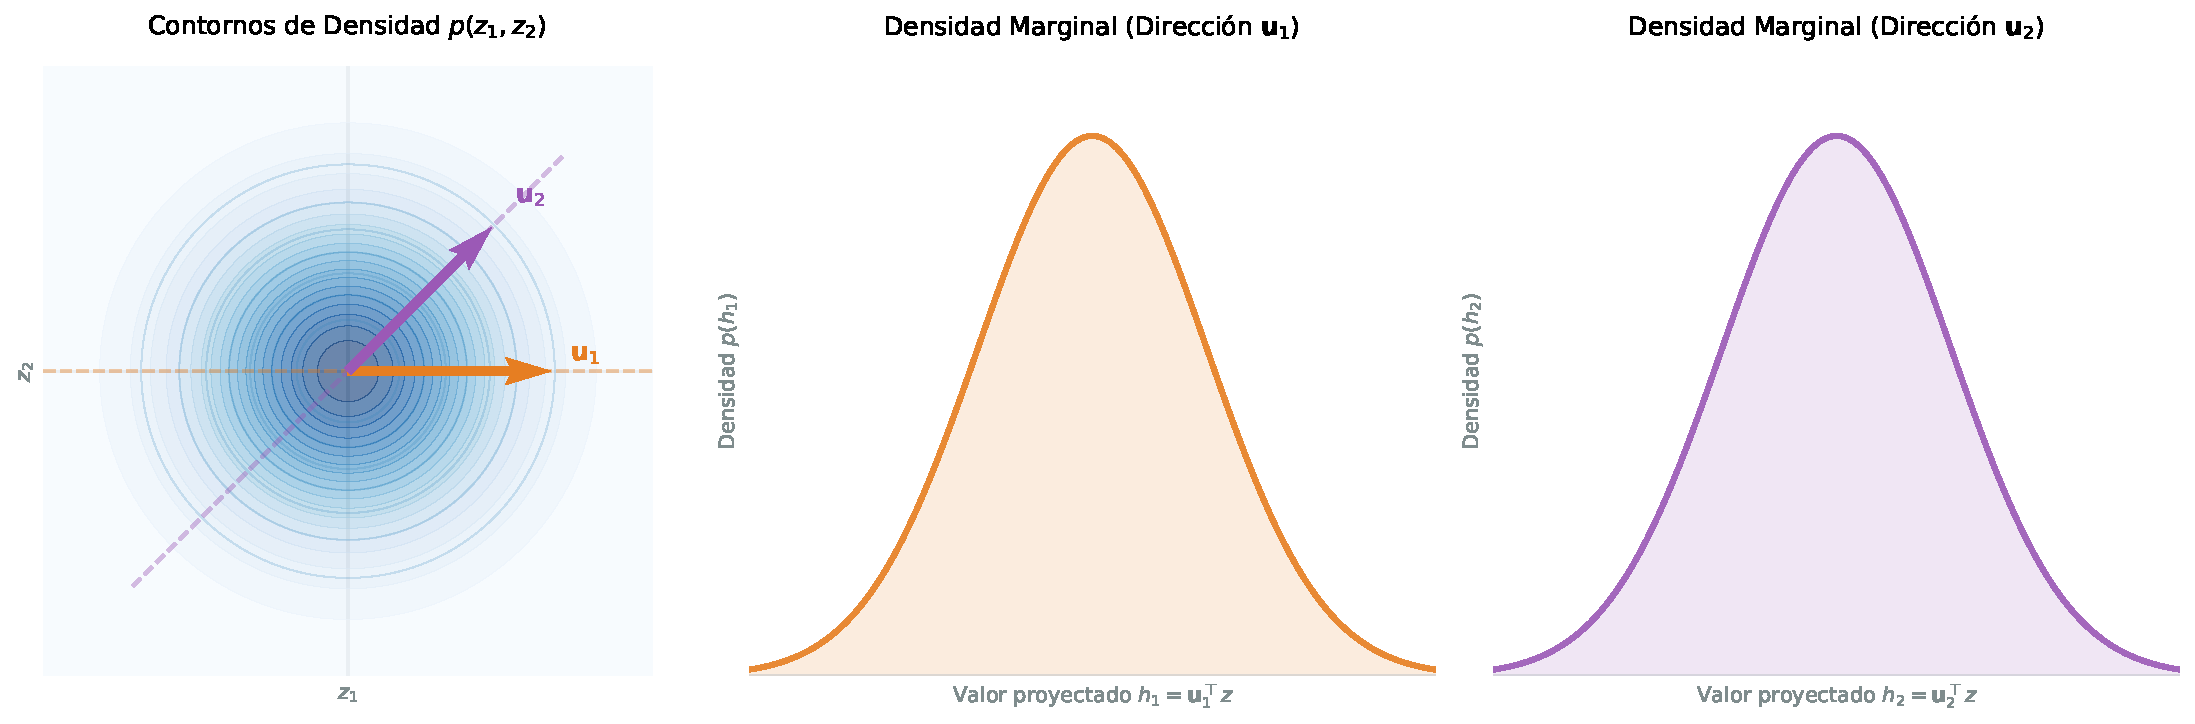
\includegraphics[width=\linewidth]{cramer_wold.pdf}
\caption{Ilustración de la descomposición de Cramér-Wold. \textbf{Izquierda:} Contornos de la densidad en el espacio latente $\mathcal{Z}$, mostrando la descomposición continua a lo largo de dos direcciones unitarias arbitrarias $\mathbf{u}_1$ y $\mathbf{u}_2$. \textbf{Centro:} Densidad marginal proyectada a lo largo de la dirección $\mathbf{u}_1$. \textbf{Derecha:} Densidad marginal proyectada a lo largo de la dirección $\mathbf{u}_2$. El teorema establece que la distribución conjunta queda caracterizada de forma única por el conjunto completo de sus proyecciones unidimensionales.}
\label{fig:cramer_wold_idea}
\end{figure}

\begin{proposition}[Caracterización de la Gaussiana Estándar por Proyecciones]
\label{prop:equivalencia_barlow}
Sea $Z \in \mathbb{R}^d$ un vector aleatorio. Las siguientes afirmaciones son equivalentes:
\begin{enumerate}
    \item[(a)] Para toda dirección $u \in \mathbb{S}^{d-1}$, la proyección $u^\top Z$ sigue una distribución $\mathcal{N}(0,1)$.
    \item[(b)] $Z \sim \mathcal{N}(\vec{0}, I_d)$.
\end{enumerate}
\end{proposition}

\begin{proof}
\textbf{(b $\implies$ a).}
Si $Z \sim \mathcal{N}(\vec 0, I_d)$, toda combinación lineal $u^\top Z$ con $\|u\|=1$ es gaussiana con media $u^\top \vec 0 = 0$ y varianza $u^\top I_d u = \|u\|^2 = 1$. Por tanto $u^\top Z \sim \mathcal{N}(0,1)$ para toda $u\in\mathbb{S}^{d-1}$.

\textbf{(a $\implies$ b).}
Sea $W \sim \mathcal{N}(\vec 0, I_d)$. Por la implicación anterior, $u^\top W \sim \mathcal{N}(0,1)$ para toda $u\in\mathbb{S}^{d-1}$, idéntico a la hipótesis (a) sobre $Z$. Así, $Z$ y $W$ tienen exactamente las mismas leyes de proyección unidimensional. Por el Teorema de Cramér-Wold (Teorema~\ref{thm:cramer_wold}), la ley conjunta de un vector aleatorio en $\mathbb{R}^d$ queda determinada de forma única por el conjunto de sus proyecciones unidimensionales. Por tanto $Z \stackrel{d}{=} W$, es decir, $Z \sim \mathcal{N}(\vec 0, I_d)$.
\end{proof}
Estos resultados suponen pasar de imponer independencia asumiendo normalidad (el Puente de Jaynes), a imponer la normalidad en toda proyección y obtener la independencia como consecuencia. Además reduce el problema de testear normalidad multivariante a la resolución de múltiples tests univariantes en $\mathbb{R}$. Falta aún un test de normalidad que sea diferenciable, es decir, compatible con el descenso de gradiente.

\section{El Test de Epps-Pulley Diferenciable}
\label{sec:epps_pulley}

La Proposición~\ref{prop:equivalencia_barlow} reduce la verificación de la normalidad isótropa de $Z \in \mathbb{R}^d$ a comprobar que cada proyección univariante $u^\top Z$ siga una distribución $\mathcal{N}(0,1)$. Todo el trabajo de esta sección transcurre, por tanto, en $\mathbb{R}$: se busca un test que determine si una variable aleatoria real se distribuye como una normal estándar. Los tests clásicos de normalidad como Shapiro-Wilk, Anderson-Darlingo Kolmogorov-Smirnov, se apoyan en la ordenación de la muestra o en la función de distribución empírica, operaciones que involucran comparaciones y máximos no diferenciables e incompatibles con el descenso de gradiente.

En 2025~\cite{balestriero2025lejepa} se propuso el uso del estadístico de Epps y Pulley~\cite{epps1983test} que, al formular el test de normalidad mediante la \textbf{funcion característica}, cumple con las propiedades de diferenciabilidad buscadas. 

\begin{definition}[Función Característica]
\label{def:funcion_caracteristica}
Sea $X$ una variable aleatoria real distribuida según $P_X$. La función característica de $X$ es la aplicación $\phi_X : \mathbb{R} \to \mathbb{C}$ dada por
\begin{equation}
\phi_X(t) \;=\; \mathbb{E}\!\left[e^{itX}\right] \;=\; \int_{-\infty}^{\infty} e^{itx}\, dP_X(x),
\end{equation}
donde $i = \sqrt{-1}$ es la unidad imaginaria.
\end{definition}

La función característica existe para toda variable aleatoria y su  satisface que: dos variables aleatorias tienen la misma distribución \emph{si y solo si} comparten la misma función característica (\textbf{Teorema de Unicidad}). Esto hace de $\phi_X$ un identificador completo de la distribución. Por tanto, comparar $\phi_X$ con la función característica de $\mathcal{N}(0,1)$ equivale exactamente a testear la normalidad de la distribución $X$.

\begin{proposition}[Función Característica de $\mathcal{N}(0,1)$]
\label{prop:cf_normal}
Si $X \sim \mathcal{N}(0,1)$, su función característica es
\begin{equation}
\phi_0(t) = e^{-t^2/2}.
\label{eq:cf_normal}
\end{equation}
\end{proposition}

\begin{proof}
Se calcula la esperanza de la Definición~\ref{def:funcion_caracteristica}:
\begin{equation*}
\phi_0(t) = \int_{-\infty}^{\infty} e^{itx}\, \frac{1}{\sqrt{2\pi}}\, e^{-x^2/2}\, dx = \frac{1}{\sqrt{2\pi}} \int_{-\infty}^{\infty} \exp\!\left(-\frac{x^2 - 2itx}{2}\right) dx.
\end{equation*}
Completando el cuadrado en el exponente, $x^2 - 2itx = (x - it)^2 + t^2$, se obtiene
\begin{equation*}
\phi_0(t) = e^{-t^2/2}\; \underbrace{\frac{1}{\sqrt{2\pi}} \int_{-\infty}^{\infty} e^{-(x-it)^2/2}\, dx}_{=\, 1} \;=\; e^{-t^2/2},
\end{equation*}
donde la integral compleja vale $1$ por Teorema Integral de Cauchy.
\end{proof}

Cabe destacar que $\phi_0$ resulta ser una función \emph{real y positiva}. Con estas herramientas, la idea del test de Epps-Pulley se formula del siguiente modo: si la variable $X$ siguiera una distribución normal estándar $\mathcal{N}(0,1)$, su función característica $\phi_X$ coincidiría con $\phi_0$ en todo punto $t \in \mathbb{R}$. Por tanto, podemos evaluar esta smilitud usando la distancia $L^2$ entre $\phi_0$ y $\phi_X$:
\begin{equation}
T \;=\; \int_{-\infty}^{\infty} \left|\phi_X(t) - \phi_0(t)\right|^2\, w(t)\, dt,
\label{eq:epps_poblacional}
\end{equation}
donde $w(t) = \sqrt{2}\, e^{-t^2}$ es un peso que concentra la comparación y hace que la integral tenga solución anlítica exacta. $T$ es cero si y solo si $\phi_X = \phi_0$ en casi todo punto, lo que por el Teorema de Unicidad equivale a $X \sim \mathcal{N}(0,1)$.

Nótese que $T$ es un funcional \emph{poblacional}: depende de la distribución verdadera de $X$. En la práctica, solo disponemos de una muestra finita de observaciones $h_1, \dots, h_n$ generadas a partir de $X$. Para testear la normalidad a partir de esta muestra, se estima la función característica poblacional mediante la \textbf{Función Característica Empírica} (FCE):
\begin{equation}
\hat{\phi}_n(t) = \frac{1}{n} \sum_{j=1}^{n} e^{i\, t\, h_j}.
\end{equation}
Al sustituir $\phi_X$ por $\hat{\phi}_n$ en el funcional poblacional~\eqref{eq:epps_poblacional} y resolver la integral ponderada de forma analítica, se obtiene la \textbf{forma cerrada} del estadístico de Epps-Pulley para la muestra:
\begin{equation}
T(h_1, \dots, h_n) = 1 + \frac{\sqrt{2}}{n^2} \sum_{j=1}^{n} \sum_{k=1}^{n} \exp\!\left(-\frac{(h_j - h_k)^2}{4}\right) - \frac{4}{\sqrt{3}\, n} \sum_{j=1}^{n} \exp\!\left(-\frac{h_j^2}{6}\right)
\label{eq:epps_cerrada}
\end{equation}

Se elige este estadístico por su \textbf{diferenciabilidad}. Como se observa en~\eqref{eq:epps_cerrada}, el estadístico es una suma de funciones exponenciales, por tanto, cada término es infinitamente diferenciable con respecto a las observaciones $h_j$. 

Esta propiedad contrasta con los tests clásicos. El estadístico de Kolmogorov-Smirnov, por ejemplo, se define como $D = \sup_t |F_n(t) - \Phi(t)|$, donde $F_n$ es la distribución empírica acumulada y $\sup$ es la operación supremo, que cuenta con discontinuidades y carece de gradientes en dichos puntos, invalidando su uso como función de pérdida para el descenso de gradiente.

\section{El Algoritmo SIGReg y la Pérdida de LeWorldModel}
\label{sec:sigreg_algoritmo}

\subsection{Del Espacio Latente a las Proyecciones Univariantes}
La sección anterior definió el estadístico empírico de Epps-Pulley para una muestra genérica unidimensional. En la práctica, esta muestra proviene de las representaciones producidas por el encoder $f_\theta$, procesadas en batches de $N$ muestras de datos durante cada iteración del optimizador.

En el contexto general del aprendizaje de representaciones, estas muestras pueden provenir de cualquier dominio. Frecuentemente, presentan una dimensión estructural $T$, como secuencias de observaciones (p.e., $T$ instantes de una secuencia de vídeo) o regiones espaciales (como $T$ parches de una imagen), generando un tensor de representaciones en $\mathbb{R}^{N \times T \times d}$. Para aplicar la regularización, este tensor se aplana en una única matriz $Z \in \mathbb{R}^{B \times d}$, con $B = N \cdot T$, que reúne las $B$ representaciones $d$-dimensionales del lote. Cada fila $z_b \in \mathbb{R}^d$ es el embedding de un elemento individual concreto (p.e. un instante específico de una trayectoria en el caso del vídeo).

Para evaluar la normalidad de $Z$ a lo largo \textbf{una dirección} $\mathbf{u} \in \mathbb{S}^{d-1}$, se calcula la proyección univariante de cada embedding:
\begin{equation}
h_b = \mathbf{u}^\top z_b, \quad b = 1, \dots, B,
\end{equation}
obteniendo un vector de $B$ valores reales (número de muestras) $\mathbf{h_u} = (h_1, \dots, h_B)^\top = Z\mathbf{u} \in \mathbb{R}^B$, es decir el lote de observaciones proyectado sobre la dirección $\mathbf{u}$. Según la Proposición~\ref{prop:equivalencia_barlow}, si estas proyecciones se distribuyen como $\mathcal{N}(0,1)$ para todas las direcciones, entonces la distribución multivariante de los datos sigue una normal isótropa $\mathcal{N}(\vec{0}, I_d)$. Dado que el vector $\mathbf{h_u}$ constituye una muestra de tamaño $B$ de la distribución a lo largo de $\mathbf{u}$, su ajuste respecto una normal estándar se puede cuantificar evaluando el estadístico de Epps-Pulley sobre estas observaciones $T(\mathbf{h_u}) = T(h_1, \dots, h_B)$. Repitiendo este proceso para todas las direcciones, se obtiene un test de normalidad multivariante isotrópa. 

\subsection{El Regularizador SIGReg}

\textbf{SIGReg} (\textit{Sketched-Isotropic-Gaussian Regularizer}) combina la reducción dimensional de Cramér-Wold con el test de Epps-Pulley. En cada paso de entrenamiento, se muestrean $M$ direcciones unitarias $\mathbf{u}^{(1)}, \dots, \mathbf{u}^{(M)}$ uniformemente en la esfera $\mathbb{S}^{d-1}$, se calculan las $M$ proyecciones univariantes
\begin{equation}
\mathbf{h}^{(m)} = Z\, \mathbf{u}^{(m)} \in \mathbb{R}^B, \quad m = 1, \dots, M,
\end{equation}
y se promedia el estadístico de Epps-Pulley sobre todas ellas:
\begin{equation}
\text{SIGReg}(Z) = \frac{1}{M} \sum_{m=1}^{M} T\!\left(\mathbf{h}^{(m)}\right).
\end{equation}
Este escalar mide cuánto se desvían las proyecciones de $Z$ respecto a la normalidad. Al minimizarlo, se fuerza a la distribución multivariante a converger hacia $\mathcal{N}(\vec{0}, I_d)$, realizando el Principio de Barlow sin necesidad de regularizar la matriz de covarianza. El resultado es un único término que sustituye simultáneamente los tres términos de VICReg y los siete de PLDM, eliminando los gradientes en conflicto descritos en la Sección~\ref{sec:inestabilidad_gradientes}.

La pérdida total para entrenar LeWorldModel de extremo a extremo es
\begin{equation}
\mathcal{L}_{\text{LeWM}} = \mathcal{L}_{\text{pred}} + \lambda\, \text{SIGReg}(Z),
\end{equation}
con $\mathcal{L}_{\text{pred}} = \frac{1}{NT} \sum_{i=1}^{N} \sum_{t=1}^{T-1} \| \hat{z}_{t+1}^{(i)} - z_{t+1}^{(i)} \|_2^2$ (Capítulo~\ref{cap:modelos_mundo}) y $\lambda > 0$ como único hiperparámetro de regularización.

\begin{figure}[H]
\centering
\resizebox{\linewidth}{!}{
\begin{tikzpicture}[
    node distance=1.5cm,
    inputbox/.style={draw, rectangle, rounded corners, minimum width=2.2cm, minimum height=0.8cm, align=center, fill=gray!5, font=\footnotesize\sffamily},
    matbox/.style={draw, rectangle, rounded corners, minimum width=2.5cm, minimum height=1cm, align=center, fill=gray!5, font=\footnotesize\sffamily},
    termbox/.style={draw, rectangle, rounded corners, minimum width=2.5cm, minimum height=1cm, align=center, font=\footnotesize\bfseries},
    arrow/.style={->, >=stealth, thick, rounded corners},
    operator/.style={draw, circle, fill=gray!10, font=\footnotesize\bfseries, inner sep=2pt}
]

% Inputs
\node[inputbox] (z_hat) at (-5.5, 0) {Predicciones (Batch)\\$\hat{Z} \in \mathbb{R}^{B \times d}$};
\node[inputbox] (z_tgt) at (-2.0, 0) {Objetivos (Batch)\\$Z \in \mathbb{R}^{B \times d}$};
\node[inputbox] (z_all) at (5.5, 0) {Representaciones (Batch)\\$Z \in \mathbb{R}^{B \times d}$};

% Pred Loss
\node[termbox, fill=red!10] (l_pred) at (-3.75, -2.5) {MSE\\{\scriptsize Error cuadrático}};
\draw[arrow] (z_hat) |- (l_pred);
\draw[arrow] (z_tgt) |- (l_pred);

% SIGReg Branch
\node[draw=blue!30, dashed, rounded corners, fill=blue!2, inner sep=10pt, minimum width=8.5cm, minimum height=4.2cm] (cw_box) at (5.5, -3.2) {};
\node[font=\footnotesize\bfseries, text=blue!80] at (3.8, -1.5) {Cramér-Wold (Proyecciones)};

\node[align=left, font=\scriptsize] (u1) at (2.5, -2.4) {$\mathbf{h}^{(1)} = Z \mathbf{u}^{(1)}$};
\node[font=\scriptsize] at (2.5, -3.2) {$\vdots$};
\node[align=left, font=\scriptsize] (uM) at (2.5, -4.0) {$\mathbf{h}^{(M)} = Z \mathbf{u}^{(M)}$};

% Insertar imagen externa en lugar de dibujar con TikZ
\node[inner sep=0pt] at (7.0, -3.2) {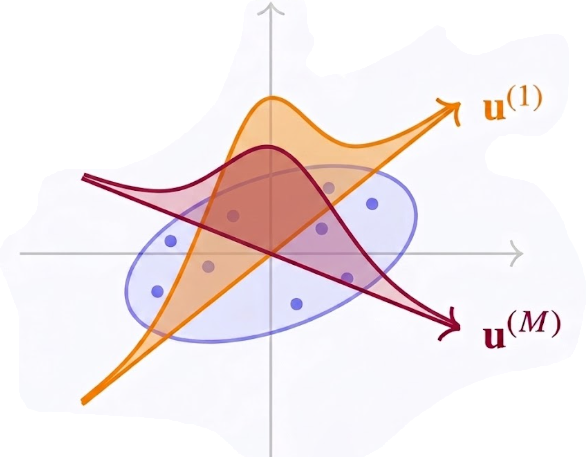
\includegraphics[width=4.5cm]{cramer_wold_new.png}};

\draw[arrow] (z_all) -- (cw_box);

% Epps-Pulley Tests
\node[matbox, fill=orange!10, draw=orange!50] (ep1) at (2.5, -6.5) {Epps-Pulley\\$T(\mathbf{h}^{(1)})$};
\node[matbox, fill=purple!10, draw=purple!50] (epM) at (8.5, -6.5) {Epps-Pulley\\$T(\mathbf{h}^{(M)})$};
\node[font=\footnotesize\bfseries] (dots) at (5.5, -6.5) {$\dots$};

\draw[arrow, orange] (2.5, -5.3) -- (ep1.north);
\draw[arrow, purple] (8.5, -5.3) -- (epM.north);

% Averaging
\node[operator] (avg) at (5.5, -8) {$\frac{1}{M} \sum$};
\draw[arrow, orange] (ep1.south) |- (avg.west);
\draw[arrow, purple] (epM.south) |- (avg.east);

% SIGReg Loss
\node[termbox, fill=blue!10] (l_sigreg) at (5.5, -9.5) {$\text{SIGReg}(Z)$\\{\scriptsize Normalidad}};
\draw[arrow] (avg) -- (l_sigreg);

% Final Total Loss
\node[operator] (plus) at (0.9, -11) {$+$};
\draw[arrow] (l_pred.south) |- (plus.west);
\draw[arrow] (l_sigreg.south) |- (plus.east);
\node[anchor=south west, font=\footnotesize] at (plus.east) {$\times \lambda$};

\node[termbox, fill=green!15, minimum width=4cm] (l_total) at (0.9, -12.5) {$\mathcal{L}_{\text{LeWM}}$\\{\scriptsize $\mathcal{L}_{\text{pred}} + \lambda \text{SIGReg}(Z)$}};
\draw[arrow] (plus) -- (l_total);

% Background Groups
\begin{scope}[on background layer]
    \node[draw=gray, dashed, rounded corners, fit=(l_pred)(z_hat)(z_tgt), inner sep=12pt, fill=gray!3] (pred_bg) {};
    \node[anchor=south, font=\footnotesize\bfseries, text=gray!60] at (pred_bg.north) {$\mathcal{L}_\text{Pred}$};
    
    \node[draw=gray, dashed, rounded corners, fit=(z_all)(cw_box)(ep1)(epM)(l_sigreg), inner sep=15pt, fill=gray!3] (sigreg_bg) {};
    \node[anchor=south, font=\footnotesize\bfseries, text=gray!60] at (sigreg_bg.north) {$\mathcal{L}_\text{SIGReg}$};
\end{scope}

\end{tikzpicture}
}
\caption{Esquema detallado de la función de pérdida de LeWorldModel. A la izquierda, la rama de predicción optimiza la similitud en el espacio latente (p.e. minimizando el error cuadrático medio). A la derecha, la rama de regularización aplica SIGReg al conjunto de representaciones del batch. Nótese que el lote de representaciones $Z \in \mathbb{R}^{B \times d}$ de la rama derecha (regularización) coincide exactamente con los objetivos reales $Z \in \mathbb{R}^{B \times d}$ de la rama izquierda (predicción): mediante Cramér-Wold se proyectan los datos multivariantes sobre múltiples direcciones aleatorias $\mathbf{u}^{(m)}$, a continuación se evalúa el ajuste a una normal univariante con el estadístico de Epps-Pulley $T$ para cada proyección, y se promedian los resultados. Ambos términos se combinan ponderados por $\lambda$.}
\label{fig:lewm_loss_schema}
\end{figure}

\begin{figure}[H]
\centering
\resizebox{\linewidth}{!}{
\begin{tikzpicture}[
    node distance=1.5cm,
    obsbox/.style={draw=gray!50, rectangle, rounded corners, minimum width=2cm, minimum height=1cm, align=center, fill=gray!5, font=\footnotesize\sffamily},
    encbox/.style={draw=blue!40, rectangle, rounded corners, minimum width=2cm, minimum height=1cm, align=center, fill=blue!5, font=\footnotesize\sffamily},
    predbox/.style={draw=violet!40, rectangle, rounded corners, minimum width=2.2cm, minimum height=1cm, align=center, fill=violet!5, font=\footnotesize\sffamily},
    lossbox/.style={draw=red!40, rectangle, rounded corners, minimum width=2.5cm, minimum height=1.2cm, align=center, fill=red!10, font=\footnotesize\bfseries},
    arrow/.style={->, >=stealth, thick, rounded corners},
    state/.style={font=\footnotesize\sffamily, align=center}
]

    % ===== FILA SUPERIOR (PASO t) =====
    \node[obsbox] (ot) at (0, 0) {Observación\\$o_t$};
    \node[encbox] (enc_t) at (2.8, 0) {Encoder\\$f_\theta$};
    \node[state] (zt) at (5.0, 0) {Estado\\$z_t$};
    \node[predbox] (pred) at (7.8, 0) {Predictor\\$g_\phi$};
    \node[state] (zhat) at (10.4, 0) {Predicción\\$\hat{z}_{t+1}$};

    % ===== FILA INFERIOR (PASO t+1) =====
    \node[obsbox] (ot1) at (0, -2.2) {Observación\\$o_{t+1}$};
    \node[encbox] (enc_t1) at (2.8, -2.2) {Encoder\\$f_\theta$};
    \node[state] (zt1) at (10.4, -2.2) {Objetivo\\$z_{t+1}$};

    % ===== CONEXIONES =====
    \draw[arrow] (ot) -- (enc_t);
    \draw[arrow] (enc_t) -- (zt);
    \draw[arrow] (zt) -- (pred);
    \draw[arrow] (pred) -- (zhat);

    \draw[arrow] (ot1) -- (enc_t1);
    \draw[arrow] (enc_t1) -- (zt1);

    % Pérdida predictiva
    \node[lossbox] (loss_asym) at (13.5, -1.1) {$\mathcal{L}_{\text{LeWM}}$};
    \draw[arrow] (zhat.east) to[out=0, in=180] (loss_asym.west);
    \draw[arrow] (zt1.east) to[out=0, in=180] (loss_asym.west);

    % Pesos compartidos
    \draw[<->, dashed, thick, gray!70] (enc_t.south) -- node[right, font=\scriptsize, text=gray!80] {pesos compartidos} (enc_t1.north);

    % Background Groups
    \begin{scope}[on background layer]
        \node[draw=orange!30, dashed, rounded corners=8pt, fit=(zt) (zhat) (pred), inner sep=10pt, fill=orange!3] (pred_zone) {};
        \node[anchor=south, font=\scriptsize\bfseries, text=orange!80] at (pred_zone.north) {Dinámica latente};
    \end{scope}

\end{tikzpicture}
}
\caption{Arquitectura base de Joint Embedding Predictiva (JEPA) utilizada en LeWorldModel. Un encoder $f_\theta$ (con pesos compartidos) extrae representaciones abstractas de las observaciones, mientras que un predictor $g_\phi$ simula la transición dinámica en el espacio latente anticipando $\hat{z}_{t+1}$ a partir del estado actual $z_t$. Posteriormente, a este modelo se le añadirá la regularización de normalidad isótropa SIGReg detallada a continuación.}
\label{fig:lewm_jepa_arch}
\end{figure}


\section{El Cierre del Círculo de Barlow}
\label{sec:conclusiones_leworldmodel}

Este capítulo culmina el recorrido evolutivo del aprendizaje de representaciones en el paradigma de Joint Embedding, resolviendo la principal limitación teórica de los métodos no contrastivos analizados en el Capítulo~\ref{cap:nocontrastive}.

El principio de reducción de redundancia de Barlow~\cite{barlow1961possible} exige la independencia estadística mutua entre las variables latentes. Bajo el marco clásico de Barlow Twins y VICReg, esta condición se aproximaba mediante la anulación de las covarianzas lineales (momentos de segundo orden), una simplificación que el Puente de Jaynes solo declara exacta bajo una hipótesis de normalidad multivariante que dichos métodos no garantizaban activamente.

A través del regularizador SIGReg se cierra de forma definitiva esta brecha:
\begin{itemize}
    \item \textbf{Fundamento en Cramér-Wold:} Permite proyectar el espacio latente de alta dimensión a múltiples direcciones unidimensionales aleatorias, reduciendo un problema multivariante intratable a una familia de evaluaciones univariantes en paralelo.
    \item \textbf{Diferenciabilidad con Epps-Pulley:} Evalúa la normalidad de cada proyección en el espacio de funciones características de manera analítica y plenamente diferenciable, forzando a la distribución latente a converger de forma suave hacia una Gaussiana isótropa.
\end{itemize}

Al asegurar de manera activa la normalidad esférica de las representaciones, la decorrelación lineal y la independencia estadística se vuelven equivalentes. De este modo, SIGReg no solo simplifica la complejidad computacional y elimina los gradientes en conflicto de VICReg, sino que aplica el principio de Barlow en su pureza matemática original.

La Figura~\ref{fig:arco_narrativo} sintetiza el flujo conceptual completo que vertebra los Capítulos~\ref{cap:siamesas_colapso}--\ref{cap:leworldmodel}.


\begin{figure}[H]
\centering
\resizebox{\linewidth}{!}{%
\begin{tikzpicture}[
    node distance=0.5cm,
    problem/.style={draw=red!70!black, rounded corners, minimum width=2cm, minimum height=1.2cm, align=center, fill=red!8, font=\scriptsize, text=black},
    solution/.style={draw=blue!70!black, rounded corners, minimum width=2cm, minimum height=1.2cm, align=center, fill=blue!8, font=\scriptsize, text=black},
    assumption/.style={draw=yellow!70!black, rounded corners, minimum width=2cm, minimum height=1.2cm, align=center, fill=yellow!10, font=\scriptsize, text=black},
    final/.style={draw=green!60!black, rounded corners, minimum width=2cm, minimum height=1.2cm, align=center, fill=green!10, font=\scriptsize, thick, text=black},
    arrow/.style={->, >=stealth, thick, gray!70},
    label/.style={font=\tiny, text=black, align=center}
]

% Nodos
\node[problem] (collapse) {Colapso\\Trivial y\\Dimensional};
\node[label, above=0.1cm of collapse] {Cap.~3\\(1993)};

\node[solution, right=of collapse] (contrastive) {P\'{e}rdidas\\Contrastivas\\$\mathcal{L}_{\text{neg}}$};
\node[label, above=0.1cm of contrastive] {Cap.~4\\(2006)};

\node[problem, right=of contrastive] (exp) {Escala\\exponencial\\$\mathcal{O}(e^d)$};

\node[solution, right=of exp] (barlow) {Barlow Twins\\VICReg\\(decorrelaci\'{o}n)};
\node[label, above=0.1cm of barlow] {Cap.~5\\(2021--2022)};

\node[assumption, right=of barlow] (gauss) {Hip\'{o}tesis\\Gaussiana\\no verificada};

\node[solution, right=of gauss] (jepa) {V-JEPA\\(heur\'{i}sticas\\ad-hoc)};
\node[label, above=0.1cm of jepa] {Cap.~6\\(2022--2025)};

\node[final, right=of jepa] (sigreg) {\textbf{SIGReg}\\Normalidad\\forzada};
\node[label, above=0.1cm of sigreg] {Cap.~7\\(2025--2026)};

% Flechas
\draw[arrow] (collapse) -- (contrastive);
\draw[arrow] (contrastive) -- (exp);
\draw[arrow] (exp) -- (barlow);
\draw[arrow] (barlow) -- (gauss);
\draw[arrow] (gauss) -- (jepa);
\draw[arrow] (jepa) -- (sigreg);

% Arco de cierre
\draw[->, >=stealth, thick, green!50!black, dashed] (sigreg.south) to[out=-90, in=-90, looseness=0.5] node[below, font=\scriptsize\itshape, text=green!50!black, yshift=-0.1cm] {Cierre del Principio de Barlow} (barlow.south);

% Leyenda
\node[below=1.8cm of collapse, font=\scriptsize, anchor=west] (leg) {
    {\tikz\draw[fill=red!8, draw=red!70!black, rounded corners] (0,0) rectangle (0.4,0.25);} Problema \quad
    {\tikz\draw[fill=blue!8, draw=blue!70!black, rounded corners] (0,0) rectangle (0.4,0.25);} Soluci\'{o}n \quad
    {\tikz\draw[fill=yellow!10, draw=yellow!70!black, rounded corners] (0,0) rectangle (0.4,0.25);} Hip\'{o}tesis pendiente \quad
    {\tikz\draw[fill=green!10, draw=green!60!black, rounded corners] (0,0) rectangle (0.4,0.25);} Resoluci\'{o}n final
};

\end{tikzpicture}%
}
\caption{Arco narrativo evolutivo de los Capítulos~\ref{cap:siamesas_colapso}--\ref{cap:leworldmodel}. Cada limitación (en rojo) motiva la solución siguiente (en azul). La hipótesis gaussiana (en amarillo), asumida implícitamente por Barlow Twins y VICReg pero nunca verificada, es finalmente impuesta de forma explícita por SIGReg (en verde), cerrando el principio de Barlow en su pureza matemática original.}
\label{fig:arco_narrativo}
\end{figure}


\section{Limitaciones, Conclusiones Generales y Líneas Futuras}
\label{sec:conclusiones_generales}

\subsection{Limitaciones del Marco SIGReg/LeWorldModel}
\label{subsec:limitaciones_sigreg}

El marco desarrollado en este capítulo resuelve la tensión planteada en la Sección~\ref{sec:limitaciones_vjepa_pldm}, pero no está libre de supuestos propios que conviene señalar con el mismo rigor con el que se han señalado los de PLDM y V-JEPA.

La primera limitación es que SIGReg fuerza la normalidad de $Z$ mediante un test estadístico diferenciable, pero la elección de la distribución objetivo, la gaussiana isótropa, no es arbitraria, sino que responde a una necesidad técnica; es la única distribución bajo la cual el Puente de Jaynes garantiza la equivalencia entre covarianza nula e independencia. Esto significa que el marco no demuestra que la normalidad sea la estructura óptima del espacio para cualquier tarea, sino que es la estructura que permite cerrar la brecha teórica identificada en la Sección~\ref{sec:barlow_hipotesis}. Si el mundo subyacente que se intenta modelar no admite una representación latente gaussiana sin pérdida de información relevante, imponer esta restricción podría limitar la expresividad de $\mathcal{Z}$.

El análisis del Puente de Jaynes desarrollado en los capítulos precedentes conduce, de forma natural, a una pregunta fundamental: ¿es la gaussianidad únicamente una propiedad que nos permite asegurar que las variables aprendidas sean estadísticamente independientes, o es además la distribución idónea para garantizar que el modelo aprenda las variables reales que describen el entorno? Esta cuestión fue resuelta recientemente por Klindt, LeCun y Balestriero, quienes demostraron formalmente que, bajo una dinámica con ruido aditivo, la distribución gaussiana es la única que permite al modelo recuperar de forma lineal las variables latentes verdaderas del sistema~\cite{klindt2026lejepa}. De este modo, la normalidad que SIGReg impone sobre $\mathcal{Z}$ no es solo una elección conveniente para justificar la independencia matemática, sino la única opción que asegura una correspondencia directa entre la representación aprendida y el estado real del mundo en esta familia de modelos. Por el contrario, si las variables reales del entorno no siguen una distribución gaussiana, este tipo de regularizadores pierde dicha garantía de recuperación, lo que sugiere que para modelar dinámicas no gaussianas se requerirían modificaciones en la arquitectura del modelo y no solo un ajuste de sus hiperparámetros~\cite{klindt2026lejepa}. Este último resultado ~\cite{klindt2026lejepa} publicado a finales de mayo de 2026 resalta cómo el problema que abordamos en el presente trabajo, se encuentra en la frontera activa de la investigación actual, habiendo evolucionado teóricamente de forma paralela a la redacción del mismo.

La segunda limitación es de naturaleza práctica. El test de Epps-Pulley diferenciable introducido en la Sección~\ref{sec:epps_pulley} evalúa la normalidad mediante proyecciones aleatorias en una dimensión, apoyándose en el Teorema de Cramér-Wold (Sección~\ref{sec:cramer_wold}). El número de proyecciones necesarias para que esta aproximación sea fiel a la normalidad multivariada completa crece con la dimensión de $\mathcal{Z}$, lo que introduce un coste computacional adicional respecto a los términos de varianza y covarianza de VICReg, que se calculan de forma cerrada.

\chapter{Conclusiones y Líneas Futuras}
\label{cap:conclusiones}

\section{El Hilo Conductor: del Colapso a su Resolución}
\label{sec:cumplimiento_objetivos}

El Capítulo~\ref{cap:intro} planteaba como hilo conductor de esta memoria la resolución del problema más persistente de este paradigma: el \textbf{representation collapse} (colapso de representación), donde la red minimiza la energía a cero mapeando todas las entradas a una constante trivial $f_{\theta}(x) = c$. Cada capítulo abordó una etapa distinta de ese problema, y conviene cerrar la memoria recorriendo el mismo orden para mostrar cómo cada etapa queda finalmente integrada en el marco de este capítulo.

El Capítulo 2 introdujo los EBMs como marco unificador para el aprendizaje de compatibilidades y sentó, a través del Principio de Máxima Entropía de Jaynes, la base física de toda asignación de probabilidades sobre $\mathcal{Z}$. Ese mismo principio reaparece aquí en su forma más concreta: la distribución gaussiana isótropa que SIGReg fuerza sobre $\mathcal{Z}$ es precisamente la distribución de máxima entropía bajo varianza fija, de modo que el marco de Jaynes introducido en el Capítulo 2 no solo fundamenta la teoría, sino que determina la elección de diseño de este capítulo final.

El Capítulo 3 demostró analíticamente la vulnerabilidad al colapso de representación de las redes siamesas cuando solo se dispone de alineamiento positivo. El Capítulo 4 mostró que el aprendizaje contrastivo evita ese colapso mediante fuerzas de repulsión basadas en muestras negativas, a costa de los límites computacionales estudiados en esa misma sección. SIGReg no pertenece a ninguna de estas dos familias: el colapso queda excluido por construcción, sin pares negativos, porque la regularización exige una varianza fija y una covarianza nula en cada dimensión de $\mathcal{Z}$.

El Capítulo 5 estudió la revolución no contrastiva inspirada en la hipótesis de Barlow, mostrando que Barlow Twins y VICReg evitan el colapso mediante regularizaciones matriciales, pero a cambio de una dependencia que ninguna de las dos arquitecturas reconoce de forma explícita: su garantía de independencia estadística solo es válida bajo normalidad de $Z$. El Capítulo 6 extendió el marco a los world models temporales y a las JEPA, mostrando que PLDM hereda esa misma dependencia gaussiana no verificada, mientras que V-JEPA evita el colapso mediante heurísticas arquitectónicas, EMA y stop-gradient, que funcionan en la práctica sin ningún principio estadístico que las respalde.

El Capítulo 7 expuso el formalismo de LeWorldModel y su simplificación probabilística de regularización isótropa, SIGReg, que utiliza el Teorema de Cramér-Wold y el test de Epps-Pulley para lograr una regularización libre de colapso. Con ello cierra el hilo conductor resolviendo la limitación teórica subyacente: fuerza, en lugar de asumir, la normalidad multivariante que Barlow Twins, VICReg y PLDM necesitaban sin garantizar para que la decorrelación implique independencia. El colapso de representación que abre la memoria en el Capítulo 3 queda así descartado en el Capítulo 7, no por una solución arquitectónica como en V-JEPA, sino por una condición estadística, rigurosa y verificable.

\section{Líneas Futuras}
\label{sec:lineas_futuras}

Esta memoria establece las bases teóricas de los \emph{world models} basados en \emph{Joint Embedding}. Su aplicación práctica, sin embargo, apenas comienza a explorarse, y las limitaciones discutidas a lo largo de este trabajo trazan dos grandes líneas de investigación y desarrollo futuras, alineadas con la visión contemporánea de H-JEPA (\emph{Hierarchical JEPA}) y su extensión a sistemas complejos.

La primera línea, y la más apremiante en el ámbito de la robótica y el control de agentes autónomos, es la transición hacia \textbf{Modelos de Mundo Jerárquicos (H-JEPA)}. Actualmente, los modelos de tipo VLA (\emph{Vision-Language-Action}) son la última tecnología en control robótico; sin embargo, dependen de la imitación del comportamiento (\emph{behavioral cloning}) y carecen de capacidad de planificación explícita al no poseer un modelo predictivo de sus propias acciones. El enfoque JEPA supera esta carencia al aprender un modelo del mundo condicionado por la acción que permite evaluar secuencias y planificar en el espacio latente. No obstante, los modelos predictivos con arquitectura plana, como LeWorldModel, se muestran inestables en horizontes de planificación largos (fallando al intentar predecir más allá de unos pocos pasos en tareas físicas simples como el entorno \emph{Push-T}~\cite{klindt2026lejepa}). Una vía prometedora hacia la solución de este problema es la predicción jerárquica, es decir, estructurar el espacio latente en múltiples niveles de abstracción. En H-JEPA, los niveles inferiores realizarían predicciones a muy corto plazo reteniendo un alto grado de detalle (necesario, por ejemplo, para el control motor de milisegundo a milisegundo), mientras que los niveles superiores operarían sobre horizontes temporales más amplios omitiendo los detalles finos e impredecibles. Las predicciones en la capa superior actúan entonces como sub-objetivos (\emph{subgoals}) para el planificador del nivel inferior. Integrar garantías probabilísticas estables como SIGReg a través de estas múltiples capas para evitar el colapso dimensional es un problema abierto y fundamental para alcanzar un verdadero razonamiento a largo plazo.

La segunda línea, no menos ambiciosa, es la aplicación de estos modelos a \textbf{sistemas dinámicos complejos}. El control óptimo clásico requiere que la dinámica del sistema pueda describirse con unas pocas ecuaciones matemáticas (como la cinemática de un brazo robótico o la dinámica de una población). Sin embargo, arquitecturas como JEPA abren la puerta a aprender simuladores latentes puramente a partir de datos observacionales en dominios donde el modelado analítico resulta intratable. Esto expande el uso de los modelos de mundo más allá de los agentes físicos y virtuales tradicionales, dirigiéndose hacia sistemas industriales como la predicción aerodinámica en motores a reacción, el control de plantas químicas o de energía, el diseño en ciencia de materiales o incluso modelos económicos y sociales complejos. A largo plazo, abarcaría incluso dominios biológicos y médicos, como planificar un curso de tratamiento personalizado simulando el estado fenotípico futuro de un paciente crónico frente a distintas intervenciones terapéuticas. En todos estos escenarios de alta complejidad predictiva, el uso de regularizadores probabilísticos para imponer una estructura estadística bien condicionada en el espacio latente (\emph{embedding space}) resulta ser un paso indispensable.

Ambas líneas convergen, en última instancia, en un mismo problema: dotar al espacio de representación de una estructura estadística que sea a la vez rica y estable, capaz de sostener la predicción sin colapsar bajo su propio peso. Si el cálculo diferencial proporcionó el lenguaje para describir los sistemas continuos de la física clásica, quizás la geometría estadística de los espacios latentes esté llamada a desempeñar un papel semejante para las máquinas que, en las próximas décadas, aprenderán a anticipar el futuro antes de actuar sobre él. Este trabajo no pretende agotar esa tarea, sino señalar, con el rigor que permite el estado actual de la teoría, una de sus primeras rutas transitables.


\appendix
\chapter{Fundamentos de Deep Learning}
\label{ap:fundamentos_dl}

Este apéndice recoge los conceptos fundamentales del aprendizaje profundo que sirven de base técnica a los desarrollos del texto principal. Se presenta como material de consulta para el lector no especializado en redes neuronales. Como referencias básicas para profundizar en estos fundamentos, remitimos al lector a: Goodfellow et al. \cite{goodfellow2016deep}, al trabajo clásico fundacional sobre retropropagación de Rumelhart et al. \cite{rumelhart1986learning}, y a la exhaustiva revisión sobre aprendizaje de representaciones de Bengio et al. \cite{bengio2013representation}.

\section{El Perceptrón Multicapa (MLP)}
\label{sec:mlp}

El bloque constructivo fundamental de las arquitecturas utilizadas en este trabajo es la \textbf{red neuronal feedforward} o Perceptrón Multicapa (MLP, \textit{Multilayer Perceptron}) \cite{goodfellow2016deep}. Un MLP de $L$ capas ocultas define una aplicación parametrizada $f_\theta: \mathbb{R}^{d_0} \to \mathbb{R}^{d_L}$ mediante la composición de transformaciones afines y no linealidades:

\begin{definition}[Red Neuronal Feedforward]
Sea $d_0, d_1, \ldots, d_L \in \mathbb{N}$ la secuencia de dimensiones de cada capa. Para cada capa $\ell = 1, \ldots, L$, se definen una matriz de pesos $W^{(\ell)} \in \mathbb{R}^{d_\ell \times d_{\ell-1}}$ y un vector de sesgo $b^{(\ell)} \in \mathbb{R}^{d_\ell}$. La \textbf{propagación hacia adelante} (\textit{feedforward pass}) se define recursivamente como:
\begin{equation}
\label{eq:feedforward}
h^{(0)} = x, \qquad
h^{(\ell)} = \sigma\!\left(W^{(\ell)} h^{(\ell-1)} + b^{(\ell)}\right), \quad \ell = 1, \ldots, L-1, \qquad
f_\theta(x) = W^{(L)} h^{(L-1)} + b^{(L)}
\end{equation}
donde $\sigma: \mathbb{R} \to \mathbb{R}$ es una función de activación no lineal aplicada elemento a elemento. El conjunto de parámetros entrenables es $\theta = \{W^{(\ell)}, b^{(\ell)}\}_{\ell=1}^{L}$.
\end{definition}

Las funciones de activación más comunes son:
\begin{itemize}
    \item \textbf{ReLU} (\textit{Rectified Linear Unit}): $\sigma(z) = \max(0, z)$. Es la función de activación por defecto en la mayoría de arquitecturas modernas por su eficiencia computacional y la ausencia del problema del gradiente que se desvanece.
    \item \textbf{Sigmoide}: $\sigma(z) = (1 + e^{-z})^{-1} \in (0,1)$. Históricamente usada en capas de salida para clasificación binaria.
    \item \textbf{GeLU} (\textit{Gaussian Error Linear Unit}): $\sigma(z) = z \cdot \Phi(z)$, donde $\Phi$ es la CDF de la normal estándar. Utilizada en Transformers.
\end{itemize}

La composición de transformaciones afines y no linealidades en \eqref{eq:feedforward} dota al MLP de \textbf{capacidad de aproximación universal}: bajo condiciones suaves, cualquier función continua puede aproximarse con precisión arbitraria aumentando la anchura o profundidad de la red \cite{goodfellow2016deep}.

\subsection{Capa de Proyección Final y Características Pre-Activación}
\label{subsec:capa_proyeccion}

En el análisis teórico de las arquitecturas de aprendizaje profundo (como se realiza en el estudio del colapso dimensional), es común abstraer toda la complejidad no lineal de las primeras $L-1$ capas y centrar el análisis matemático riguroso en la dinámica de la última capa de la red. Para ello, la función global de la red neuronal se descompone conceptualmente en dos partes. Primero, un \textit{feature extractor} o encoder no lineal que engloba todas las capas intermedias y mapea la entrada original $x$ a un vector de características pre-activación (o representaciones profundas), denotado como $\phi(x) \in \mathbb{R}^m$. Segundo, una \textbf{capa de proyección final} puramente lineal parametrizada por una matriz de pesos $W \in \mathbb{R}^{d \times m}$. Omitiendo el término de bias por simplicidad geométrica y analítica (una práctica estándar en teoría de aprendizaje profundo), la salida completa de la red se puede expresar de forma compacta como el producto:
\begin{equation}
    f_W(x) = W \phi(x)
\end{equation}
Esta parametrización lineal resulta ser una herramienta analítica extremadamente poderosa, que permite aislar y estudiar la dinámica de evolución de los pesos finales $W$ durante el entrenamiento, expresando las fuerzas de optimización del gradiente directamente en función de la matriz de covarianza de las representaciones $\phi(x)$.

\section{Funciones de Pérdida}
\label{sec:loss_functions}

El entrenamiento de una red neuronal consiste en encontrar los parámetros $\theta^*$ que minimizan una \textbf{función de pérdida} $\mathcal{L}(\theta)$ que mide la discrepancia entre las predicciones del modelo y la señal de supervisión disponible.

\subsection{Error Cuadrático Medio (MSE)}
\label{subsec:mse}

En tareas de regresión, la pérdida de mínimos cuadrados es la elección estándar. Dado un conjunto de datos $\{(x_i, y_i)\}_{i=1}^N$:
\begin{equation}
\label{eq:mse}
\mathcal{L}_{\text{MSE}}(\theta) = \frac{1}{N} \sum_{i=1}^N \| f_\theta(x_i) - y_i \|_2^2
\end{equation}
Como se discute en la Sección~\ref{subsec:generativo} del Capítulo~\ref{cap:intro}, la minimización de \eqref{eq:mse} bajo incertidumbre multimodal fuerza al modelo a predecir la esperanza condicional, lo que produce el efecto de borrosidad en visión.

\subsection{Entropía Cruzada}
\label{subsec:cross_entropy}

Para tareas de clasificación con $C$ clases, se utiliza la función de pérdida de \textbf{entropía cruzada}, que mide la divergencia KL entre la distribución real $p$ y la predicha por el modelo $q_\theta$:
\begin{equation}
\label{eq:cross_entropy}
\mathcal{L}_{\text{CE}}(\theta) = -\frac{1}{N} \sum_{i=1}^N \sum_{c=1}^C y_{ic} \log q_\theta(c \mid x_i)
\end{equation}
donde $q_\theta(c \mid x_i) = \text{softmax}(f_\theta(x_i))_c$ es la probabilidad predicha por el modelo para la clase $c$. Esta función es el análogo discreto de la log-verosimilitud negativa bajo la distribución de Gibbs-Boltzmann de \eqref{eq:boltzmann_dist}.

\subsection{Aproximación por Minibatches}
\label{subsec:minibatch}

En el aprendizaje profundo, evaluar la expectativa matemática de una pérdida $\mathcal{L}(x)$ sobre la distribución completa de datos $p(x)$ (o sobre un conjunto de entrenamiento completo de gran cardinalidad $N$) resulta computacionalmente prohibitivo. Por ello, se recurre a la aproximación empírica mediante minilotes o \emph{minibatches}.

Dado un subconjunto de datos $\mathcal{B} = \{x_i\}_{i=1}^B \subset \mathcal{X}$ de tamaño $B \ll N$ extraído uniformemente de la distribución de entrenamiento, la esperanza matemática de la pérdida se aproxima mediante el promedio empírico sobre dicho lote:
\begin{equation}
\label{eq:minibatch_approx}
\mathbb{E}_{x \sim p(x)} [\mathcal{L}(x)] \approx \frac{1}{B} \sum_{i=1}^B \mathcal{L}(x_i)
\end{equation}
Este promedio proporciona un estimador insesgado de la pérdida total y del gradiente con respecto a los parámetros, reduciendo la carga de memoria y posibilitando la paralelización eficiente en aceleradores de hardware.

\section{Retropropagación del Error (Backpropagation)}
\label{sec:backprop}

El algoritmo de \textbf{retropropagación} \cite{rumelhart1986learning} es el procedimiento que permite calcular eficientemente el gradiente $\nabla_\theta \mathcal{L}(\theta)$ respecto a todos los parámetros de la red, habilitando el entrenamiento por descenso de gradiente.

\subsection{La Regla de la Cadena en Grafos Computacionales}
\label{subsec:regla_cadena}

La retropropagación es una aplicación sistemática de la regla de la cadena del cálculo diferencial a la estructura compositiva del MLP. Para una función compuesta $\mathcal{L} = \ell \circ f^{(L)} \circ \cdots \circ f^{(1)}$, el gradiente respecto a los parámetros de la capa $\ell$ se obtiene propagando el gradiente de la pérdida hacia atrás a través de las capas:
\begin{equation}
\label{eq:backprop_chain}
\frac{\partial \mathcal{L}}{\partial W^{(\ell)}} = \frac{\partial \mathcal{L}}{\partial h^{(\ell)}} \cdot \frac{\partial h^{(\ell)}}{\partial W^{(\ell)}} = \delta^{(\ell)} \cdot \left(h^{(\ell-1)}\right)^\top
\end{equation}
donde $\delta^{(\ell)} = \frac{\partial \mathcal{L}}{\partial h^{(\ell)}}$ es el \textbf{error local} de la capa $\ell$, que se calcula recursivamente desde la última capa:
\begin{equation}
\label{eq:delta_recurse}
\delta^{(L)} = \nabla_{h^{(L)}} \mathcal{L}, \qquad \delta^{(\ell)} = \left(W^{(\ell+1)}\right)^\top \delta^{(\ell+1)} \odot \sigma'\!\left(W^{(\ell)} h^{(\ell-1)} + b^{(\ell)}\right)
\end{equation}
donde $\odot$ es el producto de Hadamard (elemento a elemento) y $\sigma'$ es la derivada de la función de activación. La complejidad computacional de una pasada completa hacia adelante y hacia atrás es $\mathcal{O}\!\left(\sum_\ell d_\ell \cdot d_{\ell-1}\right)$, lineal en el número de parámetros.

\subsection{Descenso de Gradiente Estocástico (SGD) y Adam}
\label{subsec:optimizers}

Una vez calculados los gradientes mediante \eqref{eq:backprop_chain}--\eqref{eq:delta_recurse}, los parámetros se actualizan iterativamente. La regla de actualización del \textbf{Descenso de Gradiente Estocástico} (SGD) es:
\begin{equation}
\label{eq:sgd}
\theta_{t+1} = \theta_t - \eta \, \nabla_\theta \mathcal{L}_{\mathcal{B}_t}(\theta_t)
\end{equation}
donde $\eta > 0$ es la tasa de aprendizaje y $\mathcal{L}_{\mathcal{B}_t}$ es la pérdida evaluada sobre un minilote $\mathcal{B}_t$ de muestras elegidas aleatoriamente. En la práctica, el optimizador más utilizado es \textbf{Adam} \cite{goodfellow2016deep}, que mantiene medias exponenciales del gradiente y del cuadrado del gradiente para adaptar la tasa de aprendizaje de forma individual para cada parámetro, obteniendo una convergencia más rápida y robusta que SGD puro.

\chapter{Nociones de Álgebra Lineal}
\label{ap:algebra_lineal}

Este anexo recopila los conceptos fundamentales de álgebra lineal utilizados a lo largo de este trabajo para el análisis del colapso dimensional y la dinámica del aprendizaje en arquitecturas siamesas. Su objetivo no es proporcionar un tratamiento exhaustivo de la teoría espectral o del cálculo matricial, sino asentar la notación y recordar los teoremas clave sobre los que descansan las demostraciones del Capítulo~\ref{cap:siamesas_colapso}.

\section{Matriz de Covarianza, Rango y Núcleo}
\label{sec:al_covarianza_rango}

En el contexto del aprendizaje de representaciones, trabajamos con variables aleatorias multidimensionales. Sea $Z$ un vector aleatorio que habita en el espacio euclídeo $\mathbb{R}^d$ (por ejemplo, el vector de activaciones o \textit{embedding} generado por la capa de salida de una red neuronal, donde $d$ es el número de neuronas), denotado como $Z = f_W(X)$, y con vector de medias $\mu = \mathbb{E}[Z]$. La \textbf{matriz de covarianza poblacional} se define como:
\begin{equation}
    \Sigma_\mathcal{Z} = \mathbb{E}\left[(Z - \mu)(Z - \mu)^T\right] \in \mathbb{R}^{d \times d}
\end{equation}

Esta matriz encapsula la estructura geométrica de la distribución de los embeddings. Por construcción, $\Sigma_\mathcal{Z}$ es una matriz \textbf{simétrica} ($\Sigma_\mathcal{Z} = \Sigma_\mathcal{Z}^T$) y \textbf{semidefinida positiva} ($v^T \Sigma_\mathcal{Z} v \ge 0$ para todo $v \in \mathbb{R}^d$). La forma cuadrática $v^T \Sigma_\mathcal{Z} v$ representa la varianza de la proyección escalar de los datos sobre la dirección unidimensional $v$:
\begin{equation}
    \operatorname{Var}(v^T Z) = v^T \Sigma_\mathcal{Z} v
\end{equation}

El \textbf{núcleo} (o espacio nulo) de $\Sigma_\mathcal{Z}$, denotado como $\operatorname{Ker}(\Sigma_\mathcal{Z})$, es un \textbf{subespacio vectorial} de $\mathbb{R}^d$ compuesto por las direcciones a lo largo de las cuales la representación no tiene varianza:
\begin{equation}
    \operatorname{Ker}(\Sigma_\mathcal{Z}) = \{ v \in \mathbb{R}^d \mid \Sigma_\mathcal{Z} v = 0 \}
\end{equation}
Dado que la varianza es nula para cualquier $v \in \operatorname{Ker}(\Sigma_\mathcal{Z})$, la proyección $v^T Z$ es constante casi seguramente, es decir, no se desvía de su media $v^T \mu$. Geométricamente, esto significa que las representaciones quedan confinadas en un \textbf{subespacio afín} (un subespacio vectorial trasladado por el vector $\mu$). En el contexto de las redes neuronales, esto implica que el modelo colapsa toda la información a un único valor a lo largo de esas direcciones; estas componentes (neuronas o combinaciones lineales de ellas) se vuelven funcionalmente inútiles (véase Sección~\ref{sec:colapso_dimensional_v2}).

Por el \textbf{Teorema del Rango-Nulidad}, para cualquier matriz cuadrada de dimensión $d$:
\begin{equation}
    d = \operatorname{rango}(\Sigma_\mathcal{Z}) + \dim(\operatorname{Ker}(\Sigma_\mathcal{Z}))
\end{equation}
Por tanto, un rango deficiente ($\operatorname{rango}(\Sigma_\mathcal{Z}) = r < d$) implica inevitablemente la existencia de un subespacio nulo de dimensión $d-r$. A este fenómeno se le conoce como \textbf{colapso dimensional}.

\section{Teorema Espectral para Matrices Simétricas}
\label{sec:al_teorema_espectral}

El Teorema Espectral es posiblemente el resultado más relevante del álgebra lineal para el análisis de componentes principales y la dinámica del descenso de gradiente.

\begin{theorem}[Teorema Espectral]
Toda matriz simétrica con coeficientes reales $A \in \mathbb{R}^{d \times d}$ es diagonalizable mediante una matriz ortogonal. Es decir, existe una matriz ortogonal $Q$ ($Q^TQ = QQ^T = I$) y una matriz diagonal $\Lambda$ tales que:
\begin{equation}
    A = Q \Lambda Q^T
\end{equation}
donde las columnas de $Q$ son una base ortonormal de autovectores de $A$, y los elementos de la diagonal de $\Lambda$ son los correspondientes autovalores reales $\lambda_i$.
\end{theorem}

Si además la matriz es semidefinida positiva (como ocurre con cualquier matriz de covarianza $\Sigma_\mathcal{Z}$), todos sus autovalores son no negativos ($\lambda_i \ge 0$). El rango de la matriz coincide exactamente con el número de autovalores estrictamente positivos.

Este teorema permite desacoplar los sistemas de ecuaciones diferenciales lineales que gobiernan la dinámica del aprendizaje en redes lineales profundas. Mediante un simple cambio de base definido por $Q$, el comportamiento complejo y acoplado de los pesos se descompone en $d$ ecuaciones escalares independientes a lo largo de las direcciones principales de los datos.

\section{Flujo de Gradiente y Desacoplamiento Espectral}
\label{sec:al_flujo_gradiente}

En la práctica, el entrenamiento de redes neuronales se realiza mediante algoritmos de optimización discretos, como el Descenso de Gradiente. Si denotamos por $\eta$ la tasa de aprendizaje (\textit{learning rate}) y $\mathcal{L}(W)$ la función de pérdida, la regla de actualización para la matriz de pesos $W$ en la iteración $t$ es:
\begin{equation}
    W_{t+1} = W_t - \eta \nabla_W \mathcal{L}(W_t)
\end{equation}

Esta ecuación puede reescribirse algebraicamente formando un cociente de diferencias finitas:
\begin{equation}
    \frac{W_{t+1} - W_t}{\eta} = - \nabla_W \mathcal{L}(W_t)
\end{equation}

Para facilitar el análisis matemático riguroso, en la teoría del aprendizaje profundo es común estudiar el límite temporal continuo de este proceso. Al tomar el límite cuando el tamaño del paso de aprendizaje se vuelve infinitesimal ($\eta \to 0$), el término izquierdo converge a la derivada temporal $\frac{dW(t)}{dt} \equiv \dot{W}(t)$. Así se obtiene la ecuación diferencial ordinaria (EDO) que rige la dinámica continua, conocida como \textbf{flujo de gradiente} (\textit{gradient flow}):
\begin{equation}
    \dot{W}(t) = -\nabla_W \mathcal{L}(W(t))
\end{equation}

Cuando el gradiente de la pérdida es lineal respecto a $W$, por ejemplo $\nabla_W \mathcal{L}(W) = W \Sigma$, obtenemos una EDO matricial acoplada de la forma $\dot{W}(t) = -W(t) \Sigma$. Aplicando el Teorema Espectral a la matriz simétrica $\Sigma = Q \Lambda Q^T$, podemos introducir el cambio de variables ortogonal $\tilde{W}(t) = W(t)Q$, transformando el sistema en:
\begin{equation}
    \dot{\tilde{W}}(t) = -\tilde{W}(t)\Lambda
\end{equation}
Esta formulación está completamente diagonalizada. Para cada entrada escalar $\tilde{w}_{ij}$, la ecuación resultante es un decaimiento exponencial simple: $\dot{\tilde{w}}_{ij}(t) = -\lambda_j \tilde{w}_{ij}(t)$, cuya solución exacta es:
\begin{equation}
    \tilde{w}_{ij}(t) = \tilde{w}_{ij}(0) e^{-\lambda_j t}
\end{equation}
Esta expresión matemática revela que la velocidad de convergencia (o contracción) está controlada exclusivamente por el espectro de $\Sigma$. Los autovalores grandes ($\lambda_j \gg 0$) provocan que los componentes del peso decaigan rápidamente hacia el origen, mientras que las direcciones del subespacio nulo ($\lambda_j = 0$) permanecen intactas. Este fenómeno es central para entender cómo las arquitecturas siamesas descartan características (véase la discusión sobre el Operador de Contracción en la Sección~\ref{sec:colapso_dimensional_v2}).


\backmatter

\bibliographystyle{acm}
\bibliography{referencias}

\end{document}
